%\vspace{-10 cm}
\chapter{出埃及}
\vspace{-1 cm}
\section{神預備摩西 1-4 }
\subsection{摩西出生 1:1-2:10}
\noindent
\subsubsection{以色列人生養眾多,被埃及新王苦害 1:1-14}
以色列的眾子各帶家眷和雅各一同來到埃及，他們的名字記在下面。 2 有魯本、西緬、利未、猶大、 3 以薩迦、西布倫、便雅憫、 4 但、拿弗他利、迦得、亞設。 5 凡從雅各而生的，共有七十人。約瑟已經在埃及。 6 約瑟和他的弟兄，並那一代的人都死了。 7 以色列人生養眾多，並且繁茂，極其強盛，滿了那地。

%\subsubsection{埃及新王苦害以色列 1:8-14}
有不認識約瑟的新王起來，治理埃及， 9 對他的百姓說：「看哪，這以色列民比我們還多，又比我們強盛。 10 來吧，我們不如用巧計待他們，恐怕他們多起來，日後若遇什麼爭戰的事，就聯合我們的仇敵攻擊我們，離開這地去了。」 11 於是埃及人派督工的轄制他們，加重擔苦害他們。他們為法老建造兩座積貨城，就是比東和蘭塞。 12 只是越發苦害他們，他們越發多起來，越發蔓延，埃及人就因以色列人愁煩。 13 埃及人嚴嚴地使以色列人做工， 14 使他們因做苦工覺得命苦。無論是和泥，是做磚，是做田間各樣的工，在一切的工上都嚴嚴地待他們。

\subsubsection{收生婆存留男孩的性命 1:15-22}
\noindent
有希伯來的兩個收生婆，一名施弗拉，一名普阿。埃及王對她們說： 16 「你們為希伯來婦人收生，看她們臨盆的時候，若是男孩，就把他殺了，若是女孩，就留她存活。」 17 但是收生婆敬畏神，不照埃及王的吩咐行，竟存留男孩的性命。 18 埃及王召了收生婆來，說：「你們為什麼做這事，存留男孩的性命呢？」 19 收生婆對法老說：「因為希伯來婦人與埃及婦人不同，希伯來婦人本是健壯的(活潑的)，收生婆還沒有到，她們已經生產了。」 20 神厚待收生婆。以色列人多起來，極其強盛。 21 收生婆因為敬畏神，神便叫她們成立家室。 22 法老吩咐他的眾民說：「以色列人所生的男孩，你們都要丟在河裡；一切的女孩，你們要存留她的性命。」

\subsubsection{摩西出生 2:1-10}

\begin{table}[H]
\centering
\begin{tabular}{p{9.5cm}|p{7.0cm}}\hline\hline
\multicolumn{1}{c|}{利未母親和姐姐}&\multicolumn{1}{c}{法老的女兒}\\\hline
有一個利未家的人娶了一個利未女子為妻。那女人懷孕，生一個兒子，見他俊美，就藏了他三個月。後來不能再藏，就取了一個蒲草箱，抹上石漆和石油，將孩子放在裡頭，把箱子擱在河邊的蘆荻中。孩子的姐姐遠遠站著，要知道他究竟怎麼樣。&法老的女兒來到河邊洗澡，她的使女們在河邊行走。她看見箱子在蘆荻中，就打發一個婢女拿來。她打開箱子，看見那孩子。孩子哭了，她就可憐他，說：「這是希伯來人的一個孩子。」 \\\hline
孩子的姐姐對法老的女兒說：「我去在希伯來婦人中叫一個奶媽來，為你奶這孩子，可以不可以？」&法老的女兒說：「可以。」\\\hline
童女就去叫了孩子的母親來。&法老的女兒對她說：「你把這孩子抱去，為我奶他，我必給你工價。」\\\hline
婦人就抱了孩子去奶他。孩子漸長，婦人把他帶到法老的女兒那裡，就做了她的兒子。&她給孩子起名叫摩西，意思說：「因我把他從水裡拉出來。」\\\hline
\end{tabular}
\end{table}

\iffalse
\begin{table}[H]
\begin{threeparttable}
\begin{tabular}{@{}p{0.55\textwidth}*{4}{L{\dimexpr0.56\linewidth-10\tabcolsep\relax}}@{}}\toprule
孩子的利未母親和姐姐 &法老的女兒 \\\hline
有一個利未家的人娶了一個利未女子為妻。那女人懷孕，生一個兒子，見他俊美，就藏了他三個月。後來不能再藏，就取了一個蒲草箱，抹上石漆和石油，將孩子放在裡頭，把箱子擱在河邊的蘆荻中。孩子的姐姐遠遠站著，要知道他究竟怎麼樣。&法老的女兒來到河邊洗澡，她的使女們在河邊行走。她看見箱子在蘆荻中，就打發一個婢女拿來。她打開箱子，看見那孩子。孩子哭了，她就可憐他，說：「這是希伯來人的一個孩子。」  \tabularnewline \hline
孩子的姐姐對法老的女兒說：「我去在希伯來婦人中叫一個奶媽來，為你奶這孩子，可以不可以？」&法老的女兒說：「可以。」 \tabularnewline \hline
童女就去叫了孩子的母親來。&法老的女兒對她說：「你把這孩子抱去，為我奶他，我必給你工價。」．\tabularnewline \hline
婦人就抱了孩子去奶他。孩子漸長，婦人把他帶到法老的女兒那裡，就做了她的兒子。&她給孩子起名叫摩西，意思說：「因我把他從水裡拉出來。」\tabularnewline \hline
\bottomrule
\end{tabular}
%\end{tabularx}
%\caption{摩西出生}
\end{threeparttable}
\end{table} 
\fi

\subsection{摩西逃往米甸 2:11-2:25}
\subsubsection{摩西殺埃及人逃往米甸 2:11-15}
後來，摩西長大，他出去到他弟兄那裡，看他們的重擔，見一個埃及人打希伯來人的一個弟兄。 12 他左右觀看，見沒有人，就把埃及人打死了，藏在沙土裡。 13 第二天他出去，見有兩個希伯來人爭鬥，就對那欺負人的說：「你為什麼打你同族的人呢？」 14 那人說：「誰立你做我們的首領和審判官呢？難道你要殺我，像殺那埃及人嗎？」摩西便懼怕，說：「這事必是被人知道了。」 15 法老聽見這事，就想殺摩西，但摩西躲避法老，逃往米甸地居住。

\subsubsection{摩西娶西坡拉 2:16-22}
\noindent
一日，他在井旁坐下。米甸的祭司有七個女兒，她們來打水，打滿了槽，要飲父親的群羊。 17 有牧羊的人來把她們趕走了，摩西卻起來幫助她們，又飲了她們的群羊。 18 她們來到父親流珥那裡，他說：「今日你們為何來得這麼快呢？」 19 她們說：「有一個埃及人救我們脫離牧羊人的手，並且為我們打水飲了群羊。」 20 他對女兒們說：「那個人在哪裡？你們為什麼撇下他呢？你們去請他來吃飯。」 21 摩西甘心和那人同住，那人把他的女兒西坡拉給摩西為妻。 22 西坡拉生了一個兒子，摩西給他起名叫革舜，意思說：「因我在外邦做了寄居的。」

\subsubsection{以色列人哀求神 2:23-25 }
過了多年，埃及王死了。以色列人因做苦工，就嘆息哀求，他們的哀聲達於神。 24 神聽見他們的哀聲，就記念他與亞伯拉罕、以撒、雅各所立的約。 25 神看顧以色列人，也知道他們的苦情。

\subsection{摩西遇見神 3:1-4:17 }
\subsubsection{摩西遇見神 3:1-6}
\begin{table}[H]
\centering
\begin{tabular}{p{7.5cm}|p{9.50cm}}\hline\hline
\multicolumn{1}{c|}{摩西}&\multicolumn{1}{c}{神}\\\hline
摩西牧養他岳父米甸祭司葉忒羅的羊群，一日領羊群往野外去，到了神的山，就是何烈山 & 耶和華的使者從荊棘裡火焰中向摩西顯現,摩西觀看，不料，荊棘被火燒著，卻沒有燒毀\\\hline
我要過去看這大異象、這荊棘為何沒有燒壞呢 &耶和華神見他過去要看，就從荊棘裡呼叫說： 摩西、摩西\\\hline
我在這裡&不要近前來,當把你腳上的鞋脫下來.因為你所站之地是聖地．我是你父親的神、是亞伯拉罕的神、以撒的神、雅各的神。\\\hline
摩西蒙上臉、因為怕看神。&\\\hline
\end{tabular}
\end{table}



%\vspace{-0.8 cm}
\subsubsection{遣摩西領以色列人出埃及 3:7-22}
\begin{table}[H]
\begin{threeparttable}
\begin{tabular}{@{}p{0.23\textwidth}*{4}{L{\dimexpr0.9\linewidth-10\tabcolsep\relax}}@{}}
\toprule
摩西 &  神 \\\hline
&耶和華說：我的百姓在埃及所受的困苦、我實在看見了．他們因受督工的轄制所發的哀聲、我也聽見了．我原知道他們的痛苦。我下來是要救他們脫離埃及人的手、領他們出了那地、到美好寬闊流奶與蜜之地、就是到迦南人、赫人、亞摩利人、比利洗人、希未人、耶布斯人之地。現在以色列人的哀聲達到我耳中、我也看見埃及人怎樣欺壓他們。故此我要打發你去見法老、使你可以將我的百姓以色列人從埃及領出來。\tabularnewline \hline
\vspace{-.6cm}{摩西對神說：「我是什麼人?竟能去見法老,將以色列人從埃及領出來呢?」}&神說：「我必與你同在。你將百姓從埃及領出來之後，你們必在這山上侍奉我，這就是我打發你去的證據。」\tabularnewline \hline
摩西對神說：「我到以色列&神對摩西說：「我是自有永有的。」\tabularnewline
人那裡，對他們說：『你們&又說：「你要對以色列人這樣說：『那自有的打發我到你們這裡來。』」\tabularnewline
\vspace{-3cm}{祖宗的神打發我到你們這裡來。』他們若問我說：『他叫什麼名字？』我要對他們說什麼呢？」}&神又對摩西說：「你要對以色列人這樣說：『耶和華你們祖宗的神，就是亞伯拉罕的神、以撒的神、雅各的神，打發我到你們這裡來。』耶和華是我的名，直到永遠；這也是我的紀念，直到萬代。你去招聚以色列的長老，對他們說：『耶和華你們祖宗的神，就是亞伯拉罕的神、以撒的神、雅各的神，向我顯現，說：我實在眷顧了你們，我也看見埃及人怎樣待你們。』我也說：『要將你們從埃及的困苦中領出來，往迦南人、赫人、亞摩利人、比利洗人、希未人、耶布斯人的地去，就是到流奶與蜜之地。』他們必聽你的話。你和以色列的長老要去見埃及王，對他說：『耶和華希伯來人的神遇見了我們，現在求你容我們往曠野去，走三天的路程，為要祭祀耶和華我們的神。』 我知道雖用大能的手，埃及王也不容你們去。我必伸手在埃及中間施行我一切的奇事，攻擊那地，然後他才容你們去。我必叫你們在埃及人眼前蒙恩，你們去的時候就不至於空手而去。但各婦女必向她的鄰舍並居住在她家裡的女人要金器銀器和衣裳，好給你們的兒女穿戴，這樣你們就把埃及人的財物奪去了。」\tabularnewline
\hline
\bottomrule
\end{tabular}
%\end{tabularx}
%\caption{遣摩西領以色列人出埃及}
\end{threeparttable}
\end{table} 


\subsubsection{杖變蛇,手生大痲瘋為證 4:1-9}
\begin{table}[H]
%\vspace{-.5 cm}
\begin{threeparttable}
\begin{tabular}{@{}p{0.4\textwidth}*{4}{L{\dimexpr0.725\linewidth-10\tabcolsep\relax}}@{}}
\toprule
摩西 &  神 \\\hline
摩西回答說:他們必不信我,也不聽我的話,必說:『耶和華並沒有向你顯現』&耶和華對摩西說：「你手裡是什麼？」\tabularnewline \hline
他說：「是杖。」&耶和華說：「丟在地上。」\tabularnewline\hline
\vspace{-.5cm}{他一丟下去，就變做蛇，摩西便跑開}&耶和華對摩西說:「伸出手來拿住牠的尾巴,牠必在你手中仍變為杖. 如此好叫他們信耶和華他們祖宗的神,就是亞伯拉罕的神,以撒的神,雅各的神是向你顯現了。」耶和華又對他說：「把手放在懷裡。」\tabularnewline\hline
他就把手放在懷裡,及至抽出來,不料手長了大痲瘋,有雪那樣白&耶和華又對他說：「把手放在懷裡。」\tabularnewline\hline
\vspace{-.55cm}{他就再把手放在懷裡，及至從懷裡抽出來，不料，手已經復原，與周身的肉一樣。}
&又說：「倘或他們不聽你的話，也不信頭一個神蹟，他們必信第二個神蹟。這兩個神蹟若都不信，也不聽你的話，你就從河裡取些水，倒在旱地上，你從河裡取的水必在旱地上變做血。」\tabularnewline\hline
\bottomrule
\end{tabular}
%\end{tabularx}
%\caption{手生大痲瘋為證}
\end{threeparttable}
\end{table} 

\subsubsection{摩西拒绝受差遣 4:10-17}
\begin{table}[H]
%\vspace{-.5 cm}
\begin{threeparttable}
\begin{tabular}{@{}p{0.35\textwidth}*{4}{L{\dimexpr0.75\linewidth-10\tabcolsep\relax}}@{}}
\toprule
摩西 &  神 \\\hline
\vspace{-.65cm}{摩西對耶和華說：「主啊，我素日不是能言的人，就是從你對僕人說話以後，也是這樣。我本是拙口笨舌的。」}
&耶和華對他說：「誰造人的口呢？誰使人口啞、耳聾、目明、眼瞎呢？豈不是我耶和華嗎？ 現在去吧，我必賜你口才，指教你所當說的話。」 \tabularnewline\hline
摩西說：「主啊，你願意打發誰，就打發誰去吧！」
&耶和華向摩西發怒說：「不是有你的哥哥利未人亞倫嗎？我知道他是能言的，現在他出來迎接你，他一見你，心裡就歡喜。你要將當說的話傳給他，我也要賜你和他口才，又要指教你們所當行的事。他要替你對百姓說話，你要以他當做口，他要以你當做神。你手裡要拿這杖，好行神蹟。」\tabularnewline
\hline
\bottomrule
\end{tabular}
%\end{tabularx}
%\caption{摩西拒绝受差遣}
\end{threeparttable}
\end{table} 

\subsection{摩西受差返回埃及 4:18-31}
\subsubsection{摩西辞别岳父葉忒羅 4:18}
\begin{wrapfigure}{r}{0.55\textwidth}
\vspace*{-19mm}
-\hspace*{-5mm}
\centering
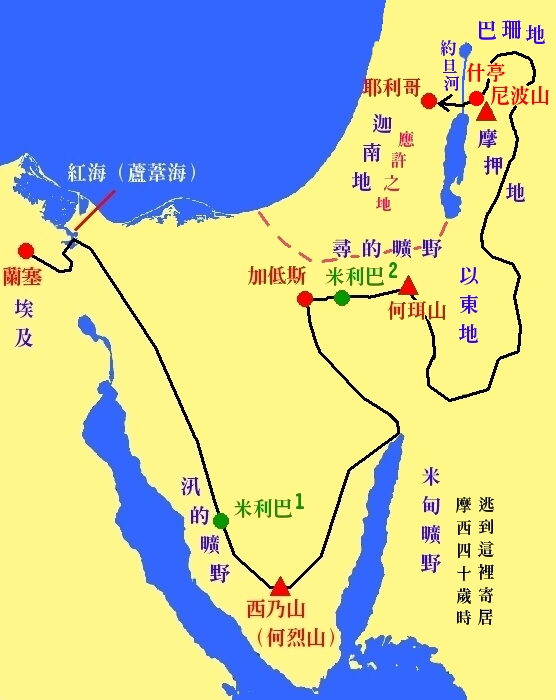
\includegraphics[width=0.8\textwidth]{AMoXiFigs/chuaiji/moses}
%\caption{以色列在曠野的經歷}
\label{fig:sub1}
\end{wrapfigure}
於是，摩西回到他岳父葉忒羅那裡，對他說：「求你容我回去見我在埃及的弟兄，看他們還在不在。」葉忒羅對摩西說：「你可以平平安安地去吧。」

\subsubsection{摩西回埃及的路上遇见神 4:19-26}

耶和華在米甸對摩西說：「你要回埃及去，因為尋索你命的人都死了。」摩西就帶著妻子和兩個兒子，叫他們騎上驢，回埃及地去。摩西手裡拿著神的杖。耶和華對摩西說：「你回到埃及的時候，要留意將我指示你的一切奇事行在法老面前。但我要使(任憑)他的心剛硬，他必不容百姓去。你要對法老說：『耶和華這樣說：以色列是我的兒子，我的長子。我對你說過容我的兒子去，好侍奉我，你還是不肯容他去。看哪，我要殺你的長子。』」摩西在路上住宿的地方，耶和華遇見他，想要殺他。西坡拉就拿一塊火石，割下他兒子的陽皮，丟在摩西腳前，說：「你真是我的血郎了！」 這樣，耶和華才放了他。西坡拉說：「你因割禮就是血郎了。」

\newpage
\subsubsection{亞倫迎接摩西 4:27-31}
耶和華對亞倫說：「你往曠野去迎接摩西。」他就去，在神的山遇見摩西，和他親嘴。 28 摩西將耶和華打發他所說的言語和囑咐他所行的神蹟都告訴了亞倫。 29 摩西、亞倫就去招聚以色列的眾長老。 30 亞倫將耶和華對摩西所說的一切話述說了一遍，又在百姓眼前行了那些神蹟。 31 百姓就信了。以色列人聽見耶和華眷顧他們，鑒察他們的困苦，就低頭下拜。


\section{以色列人出埃及 5-12}
\subsection{摩西亞倫見法老的第一回合 5:1-21}
\subsubsection{摩西亞倫初次見法老 5:1-5}
\begin{itemize} 
\itemsep-.35em 
\item 後來摩西、亞倫去對法老說：「耶和華以色列的神這樣說：『容我的百姓去，在曠野向我守節。』」法老說：「耶和華是誰，使我聽他的話，容以色列人去呢？我不認識耶和華，也不容以色列人去。」
\item 他們說：「希伯來人的神遇見了我們。求你容我們往曠野去，走三天的路程，祭祀耶和華我們的神，免得他用瘟疫、刀兵攻擊我們。」埃及王對他們說：「摩西，亞倫，你們為什麼叫百姓曠工呢？你們去擔你們的擔子吧！」又說：「看哪，這地的以色列人如今眾多，你們竟叫他們歇下擔子！」
\end{itemize}

\subsubsection{以色列人的官長受責罰 5:6-21}
\begin{itemize} 
\itemsep-.35em 
\item 當天，法老吩咐督工的和官長說：「你們不可照常把草給百姓做磚，叫他們自己去撿草。他們素常做磚的數目，你們仍舊向他們要，一點不可減少。因為他們是懶惰的，所以呼求說：『容我們去祭祀我們的神。』你們要把更重的工夫加在這些人身上，叫他們勞碌，不聽虛謊的言語。」
\item 以色列人的官長就來哀求法老說：「為什麼這樣待你的僕人？督工的不把草給僕人，並且對我們說：『做磚吧！』看哪，你僕人挨了打，其實是你百姓的錯。」 但法老說：「你們是懶惰的！你們是懶惰的！所以說：『容我們去祭祀耶和華。』現在你們去做工吧！草是不給你們的，磚卻要如數交納。」以色列人的官長聽說「你們每天做磚的工作一點不可減少」，就知道是遭遇禍患了。
\item 他們離了法老出來，正遇見摩西、亞倫站在對面，就向他們說：「願耶和華鑒察你們，施行判斷！因你們使我們在法老和他臣僕面前有了臭名，把刀遞在他們手中殺我們。」
\end{itemize}

\subsection{摩西亞倫見法老的第二回合 6:1-30}
\subsubsection{神向摩西亞倫確認應許 6:1-8}
\begin{itemize} 
\itemsep-.35em 
\item 耶和華對摩西說:現在你必看見我向法老所行的事,使他因我大能的手容以色列人去,且把他們趕出他的地
\item 神曉諭摩西說：「我是耶和華。我從前向亞伯拉罕、以撒、雅各顯現為全能的神，至於我名耶和華，他們未曾知道。我與他們堅定所立的約，要把他們寄居的迦南地賜給他們。我也聽見以色列人被埃及人苦待的哀聲，我也記念我的約。所以你要對以色列人說：我是耶和華，我要用伸出來的膀臂重重地刑罰埃及人，救贖你們脫離他們的重擔，不做他們的苦工。我要以你們為我的百姓，我也要做你們的神。你們要知道我是耶和華你們的神，是救你們脫離埃及人之重擔的。我起誓應許給亞伯拉罕、以撒、雅各的那地，我要把你們領進去，將那地賜給你們為業。我是耶和華。」
\end{itemize}

\subsubsection{人对神應許的反应 6:9-13}
\begin{itemize} 
\itemsep-.35em 
\item 摩西將這話告訴以色列人，只是他們因苦工愁煩，不肯聽他的話。
\item 耶和華曉諭摩西說： 「你進去對埃及王法老說，要容以色列人出他的地。」 
\item 摩西在耶和華面前說：「以色列人尚且不聽我的話，法老怎肯聽我這拙口笨舌的人呢？」\item 耶和華吩咐摩西、亞倫往以色列人和埃及王法老那裡去，把以色列人從埃及地領出來。
\end{itemize}

%\newpage
\subsubsection{摩西亞倫的家譜 6:14-25}
\begin{forest}
  for tree={
    child anchor=west,
    parent anchor=east,
    grow=east,
    draw,
    anchor=west,
    edge path={
      \noexpand\path[\forestoption{edge}]
        (.child anchor) -| +(-5pt,0) -- +(-5pt,0) |-
        (!u.parent anchor)\forestoption{edge label};
    },
  }
  [以色列
    [流便[哈諾] [法路] [希斯崙] [迦米]]
    [西緬[耶母利] [雅憫][阿轄][雅斤][瑣轄][掃羅（南女子的兒子）]]
    [利未（137歲）[約基別][革順[立尼][示每]] 
    					[哥轄（133歲）[暗蘭（妻子約基別）[亞倫（妻以利沙巴[拿答][亞比戶][以利亞撒[非尼哈]][以他瑪]][摩西][米利暗（姐姐）]
            ]
    									  [以斯哈[可拉[亞惜][以利加拿][亞比亞撒]][尼斐][細基利]]
    									  [希伯倫]
    									  [烏薛[米沙利][以利撒反][西提利]]] 
    					[米拉利[抹利][母示]]]                            
  ]
\end{forest}

\subsubsection{简介摩西亞倫 6:26-27}
\begin{itemize} 
\itemsep-.35em 
\item 亞倫的兒子以利亞撒娶了普鐵的一個女兒為妻，她給他生了非尼哈。這是利未人的家長，都按著他們的家
\item 耶和華說：「將以色列人按著他們的軍隊從埃及地領出來。」這是對那亞倫、摩西說的。對埃及王法老說要將以色列人從埃及領出來的，就是這摩西、亞倫。
\end{itemize}


\subsubsection{摩西亞倫受神命見法老 6:28-7:7}
\begin{itemize} 
\itemsep-.35em 
\item 當耶和華在埃及地對摩西說話的日子, 他向摩西說:我是耶和華，我對你說的一切話你都要告訴埃及王法老
\item 摩西在耶和華面前說：「看哪，我是拙口笨舌的人，法老怎肯聽我呢？」
\item 耶和華對摩西說：「我使你在法老面前代替神，你的哥哥亞倫是替你說話的。凡我所吩咐你的，你都要說。你的哥哥亞倫要對法老說，容以色列人出他的地。我要使法老的心剛硬，也要在埃及地多行神蹟奇事。但法老必不聽你們，我要伸手重重地刑罰埃及，將我的軍隊以色列民從埃及地領出來。我伸手攻擊埃及，將以色列人從他們中間領出來的時候，埃及人就要知道我是耶和華。」
\item 摩西、亞倫這樣行，耶和華怎樣吩咐他們，他們就照樣行了。摩西、亞倫與法老說話的時候，摩西八十歲，亞倫八十三歲
\end{itemize}

\subsubsection{杖變蛇為證 7:8-13}
\begin{itemize} 
\itemsep-.35em 
\item 耶和華曉諭摩西、亞倫說：「法老若對你們說：『你們行件奇事吧』，你就吩咐亞倫說：『把杖丟在法老面前，使杖變做蛇。』」
\item 摩西、亞倫進去見法老，就照耶和華所吩咐的行。亞倫把杖丟在法老和臣僕面前，杖就變做蛇。於是法老召了博士和術士來，他們是埃及行法術的，也用邪術照樣而行。他們各人丟下自己的杖，杖就變做蛇，但\underline{亞倫的杖吞了他們的杖}。
\item 法老心裡剛硬，不肯聽從摩西、亞倫，正如耶和華所說的。
\end{itemize}

\subsection{十災 6:28-12:36}



\subsubsection{水變血之災 7:14-25}
\begin{itemize} 
\itemsep-.35em 
\item 耶和華對摩西說：法老心裡固執，不肯容百姓去。明日早晨，他出來往水邊去，你要往河邊迎接他，手裡要拿著那變過蛇的杖
\begin{itemize} 
\itemsep-.35em 
\item 對他(法老)說：『耶和華希伯來人的神打發我來見你，說：「容我的百姓去，好在曠野侍奉我」，到如今你還是不聽。耶和華這樣說：我要用我手裡的杖擊打河中的水，水就變做血，因此你必知道我是耶和華。河裡的魚必死，河也要腥臭，埃及人就要厭惡吃這河裡的水。』
\item 耶和華曉諭摩西說：「你對亞倫說：『把你的杖伸在埃及所有的水以上，就是在他們的江、河、池、塘以上，叫水都變做血。在埃及遍地，無論在木器中、石器中，都必有血。』」
\end{itemize}
\item 摩西、亞倫就照耶和華所吩咐的行。亞倫在法老和臣僕眼前舉杖擊打河裡的水，河裡的水都變做血了。河裡的魚死了，河也腥臭了，埃及人就不能吃這河裡的水。埃及遍地都有了血。 
\item 埃及行法術的，也用邪術照樣而行。法老心裡剛硬，不肯聽摩西、亞倫，正如耶和華所說的。法老轉身進宮，也不把這事放在心上。埃及人都在河的兩邊挖地，要得水喝，因為他們不能喝這河裡的水。耶和華擊打河以後滿了七天。
\end{itemize}

\subsubsection{蛙災 8:1-15}
耶和華吩咐摩西說：「你進去見法老，對他說：『耶和華這樣說：容我的百姓去，好侍奉我。 2 你若不肯容他們去，我必使青蛙糟蹋你的四境。 3 河裡要滋生青蛙，這青蛙要上來進你的宮殿和你的臥房，上你的床榻，進你臣僕的房屋，上你百姓的身上，進你的爐灶和你的摶麵盆， 4 又要上你和你百姓並你眾臣僕的身上。』」

耶和華曉諭摩西說：「你對亞倫說：『把你的杖伸在江、河、池以上，使青蛙到埃及地上來。』」 6 亞倫便伸杖在埃及的諸水以上，青蛙就上來，遮滿了埃及地。 7 行法術的也用他們的邪術照樣而行，叫青蛙上了埃及地。

8 法老召了摩西、亞倫來，說：「請你們求耶和華，使這青蛙離開我和我的民，我就容百姓去祭祀耶和華。」 9 摩西對法老說：「任憑你吧！我要何時為你和你的臣僕並你的百姓祈求，除滅青蛙離開你和你的宮殿，只留在河裡呢？」 10 他說：「明天。」摩西說：「可以照你的話吧！好叫你知道沒有像耶和華我們神的。 11 青蛙要離開你和你的宮殿，並你的臣僕與你的百姓，只留在河裡。」 12 於是摩西、亞倫離開法老出去。摩西為擾害法老的青蛙呼求耶和華。 13 耶和華就照摩西的話行。凡在房裡、院中、田間的青蛙都死了。 14 眾人把青蛙聚攏成堆，遍地就都腥臭。 15 但法老見災禍鬆緩，就\textcolor{red}{硬著心}，不肯聽他們，正如耶和華所說的。


\subsubsection{蝨災 8:16-19}
耶和華吩咐摩西說：「你對亞倫說：『伸出你的杖擊打地上的塵土，使塵土在埃及遍地變做蝨子(虼蚤)。』」 17 他們就這樣行。亞倫伸杖擊打地上的塵土，就在人身上和牲畜身上有了蝨子，埃及遍地的塵土都變成蝨子了。 18 行法術的也用邪術要生出蝨子來，卻是不能。於是在人身上和牲畜身上都有了蝨子。

\subsubsection{蠅災 8:20-32}
耶和華對摩西說：「你清早起來，法老來到水邊，你站在他面前，對他說：『耶和華這樣說：容我的百姓去，好侍奉我。你若不容我的百姓去，我要叫成群的蒼蠅到你和你臣僕並你百姓的身上，進你的房屋，並且埃及人的房屋和他們所住的地都要滿了成群的蒼蠅。當那日，我必\textcolor{red}{分別}我百姓所住的歌珊地，使那裡沒有成群的蒼蠅，好叫你知道我是天下的耶和華。我要將我的百姓和你的百姓\textcolor{red}{分別}出來。明天必有這神蹟。』」耶和華就這樣行。蒼蠅成了大群，進入法老的宮殿和他臣僕的房屋，埃及遍地就因這成群的蒼蠅敗壞了。

法老召了摩西、亞倫來，說：「你們去，在這地祭祀你們的神吧！」摩西說：「這樣行本不相宜，因為我們要把埃及人所厭惡的祭祀耶和華我們的神。若把埃及人所厭惡的在他們眼前獻為祭，他們豈不拿石頭打死我們嗎？我們要往曠野去，走三天的路程，照著耶和華我們神所要吩咐我們的祭祀他。」法老說：「我容你們去，在曠野祭祀耶和華你們的神，只是不要走得很遠。求你們為我祈禱。」摩西說：「我要出去求耶和華，使成群的蒼蠅明天離開法老和法老的臣僕並法老的百姓，法老卻不可再行詭詐，不容百姓去祭祀耶和華。」 

於是摩西離開法老去求耶和華。 耶和華就照摩西的話行，叫成群的蒼蠅離開法老和他的臣僕並他的百姓，一個也沒有留下。這一次法老又\textcolor{red}{硬著心}，不容百姓去。


\subsubsection{畜疫之災 9:1-7}
耶和華吩咐摩西說：「你進去見法老，對他說：『耶和華希伯來人的神這樣說：容我的百姓去，好侍奉我。 2 你若不肯容他們去，仍舊強留他們， 3 耶和華的手加在你田間的牲畜上，就是在馬、驢、駱駝、牛群、羊群上，必有重重的瘟疫。 4 耶和華要\textcolor{red}{分別}以色列的牲畜和埃及的牲畜，凡屬以色列人的，一樣都不死。』」 5 耶和華就定了時候，說：「明天耶和華必在此地行這事。」 6 第二天，耶和華就行這事。埃及的牲畜幾乎都死了，只是以色列人的牲畜一個都沒有死。 7 法老打發人去看，誰知以色列人的牲畜連一個都沒有死。法老的心卻是\textcolor{red}{固執}，不容百姓去。

\subsubsection{人和牲畜身上起泡的瘡災 9:8-21}
耶和華吩咐摩西、亞倫說：「你們取幾捧爐灰，摩西要在法老面前向天揚起來。 9 這灰要在埃及全地變做塵土，在人身上和牲畜身上成了起泡的瘡。」 10 摩西、亞倫取了爐灰，站在法老面前。摩西向天揚起來，就在人身上和牲畜身上成了起泡的瘡。 11 行法術的在摩西面前站立不住，因為在他們身上和一切埃及人身上都有這瘡。 12 耶和華使法老的\textcolor{red}{心剛硬}，不聽他們，正如耶和華對摩西所說的。

13 耶和華對摩西說：「你清早起來，站在法老面前，對他說：『耶和華希伯來人的神這樣說：容我的百姓去，好侍奉我。 14 因為這一次我要叫一切的災殃臨到你和你臣僕並你百姓的身上，叫你知道在普天下沒有像我的。 15 我若伸手用瘟疫攻擊你和你的百姓，你早就從地上除滅了。 16 其實，我叫你存立，是特要向你顯我的大能，並要使我的名傳遍天下。 17 你還向我的百姓自高，不容他們去嗎？ 18 到明天約在這時候，我必叫重大的冰雹降下，自從埃及開國以來，沒有這樣的冰雹。 19 現在你要打發人把你的牲畜和你田間一切所有的催進來，凡在田間不收回家的，無論是人是牲畜，冰雹必降在他們身上，他們就必死。』」 20 法老的臣僕中，懼怕耶和華這話的，便叫他的奴僕和牲畜跑進家來。 21 但那不把耶和華這話放在心上的，就將他的奴僕和牲畜留在田裡。


\subsubsection{雹災 9:22-35}
耶和華對摩西說：「你向天伸杖，使埃及遍地的人身上和牲畜身上，並田間各樣菜蔬上，都有冰雹。」 23 摩西向天伸杖，耶和華就打雷下雹，有火閃到地上，耶和華下雹在埃及地上。 24 那時，雹與火摻雜，甚是厲害，自從埃及成國以來，遍地沒有這樣的。 25 在埃及遍地，雹擊打了田間所有的人和牲畜，並一切的菜蔬，又打壞田間一切的樹木。 26 唯獨以色列人所住的歌珊地沒有冰雹。
法老打發人召摩西、亞倫來，對他們說：「這一次我犯了罪了。耶和華是公義的，我和我的百姓是邪惡的。 28 這雷轟和冰雹已經夠了。請你們求耶和華，我就容你們去，不再留住你們。」 29 摩西對他說：「我一出城，就要向耶和華舉手禱告，雷必止住，也不再有冰雹，叫你知道全地都是屬耶和華的。 30 至於你和你的臣僕，我知道你們還是不懼怕耶和華神。」 31 那時，麻和大麥被雹擊打，因為大麥已經吐穗，麻也開了花。 32 只是小麥和粗麥沒有被擊打，因為還沒有長成。 33 摩西離了法老出城，向耶和華舉手禱告，雷和雹就止住，雨也不再澆在地上了。 34 法老見雨和雹與雷止住，就越發犯罪，他和他的臣僕都硬著心。 35 法老的\textcolor{red}{心剛硬}，不容以色列人去，正如耶和華藉著摩西所說的。

\subsubsection{蝗蟲之災 10:1-20}
 耶和華對摩西說：「你進去見法老。我使他和他臣僕的心剛硬，為要在他們中間顯我這些神蹟， 2 並要叫你將我向埃及人所做的事，和在他們中間所行的神蹟，傳於你兒子和你孫子的耳中，好叫你們知道我是耶和華。」 3 摩西、亞倫就進去見法老，對他說：「耶和華希伯來人的神這樣說：『你在我面前不肯自卑要到幾時呢？容我的百姓去，好侍奉我。 4 你若不肯容我的百姓去，明天我要使蝗蟲進入你的境內， 5 遮滿地面，甚至看不見地，並且吃那冰雹所剩的和田間所長的一切樹木。 6 你的宮殿和你眾臣僕的房屋，並一切埃及人的房屋，都要被蝗蟲占滿了。自從你祖宗和你祖宗的祖宗在世以來，直到今日，沒有見過這樣的災。』」摩西就轉身離開法老出去。 7 法老的臣僕對法老說：「這人為我們的網羅要到幾時呢？容這些人去侍奉耶和華他們的神吧！埃及已經敗壞了，你還不知道嗎？」 8 於是摩西、亞倫被召回來見法老，法老對他們說：「你們去侍奉耶和華你們的神，但那要去的是誰呢？」 9 摩西說：「我們要和我們老的少的、兒子女兒同去，且把羊群牛群一同帶去，因為我們務要向耶和華守節。」 10 法老對他們說：「我容你們和你們婦人孩子去的時候，耶和華與你們同在吧！你們要謹慎，因為有禍在你們眼前(你們存著惡意)。 11 不可都去，你們這壯年人去侍奉耶和華吧！因為這是你們所求的。」於是把他們從法老面前攆出去。
耶和華對摩西說：「你向埃及地伸杖，使蝗蟲到埃及地上來，吃地上一切的菜蔬，就是冰雹所剩的。」 13 摩西就向埃及地伸杖，那一晝一夜，耶和華使東風颳在埃及地上，到了早晨，東風把蝗蟲颳了來。 14 蝗蟲上來，落在埃及的四境，甚是厲害，以前沒有這樣的，以後也必沒有。 15 因為這蝗蟲遮滿地面，甚至地都黑暗了，又吃地上一切的菜蔬和冰雹所剩樹上的果子。埃及遍地，無論是樹木，是田間的菜蔬，連一點青的也沒有留下。 16 於是法老急忙召了摩西、亞倫來，說：「我得罪耶和華你們的神，又得罪了你們。 17 現在求你，只這一次，饒恕我的罪，求耶和華你們的神，使我脫離這一次的死亡。」 18 摩西就離開法老去求耶和華。 19 耶和華轉了極大的西風，把蝗蟲颳起，吹入紅海，在埃及的四境連一個也沒有留下。 20 但耶和華使法老的\textcolor{red}{心剛硬}，不容以色列人去。


\subsubsection{黑暗之災 10:21-29}
耶和華對摩西說：「你向天伸杖，使埃及地黑暗，這黑暗似乎摸得著。」 22 摩西向天伸杖，埃及遍地就烏黑了三天。 23 三天之久，人不能相見，誰也不敢起來離開本處，唯有以色列人家中都有亮光。 24 法老就召摩西來，說：「你們去侍奉耶和華，只是你們的羊群牛群要留下，你們的婦人孩子可以和你們同去。」 25 摩西說：「你總要把祭物和燔祭牲交給我們，使我們可以祭祀耶和華我們的神。 26 我們的牲畜也要帶去，連一蹄也不留下，因為我們要從其中取出來，侍奉耶和華我們的神。我們未到那裡，還不知道用什麼侍奉耶和華。」 27 但耶和華使法老的\textcolor{red}{心剛硬}，不肯容他們去。 28 法老對摩西說：「你離開我去吧！你要小心，不要再見我的面，因為你見我面的那日，你就必死！」 29 摩西說：「你說得好，我必不再見你的面了。」

\subsubsection{擊殺頭生的長子牲畜之災 11:1-12:30}
\subsubsubsection{以末次之災警告法老 11:1-10}
耶和華對摩西說：「我再使一樣的災殃臨到法老和埃及，然後他必容你們離開這地。他容你們去的時候，總要催逼你們都從這地出去。 2 你要傳於百姓的耳中，叫他們男女各人向鄰舍要金器銀器。」 3 耶和華叫百姓在埃及人眼前蒙恩，並且摩西在埃及地、法老臣僕和百姓的眼中看為極大。

4 摩西說：「耶和華這樣說：『約到半夜，我必出去巡行埃及遍地， 5 凡在埃及地，從坐寶座的法老直到磨子後的婢女所有的長子，以及一切頭生的牲畜，都必死。 6 埃及遍地必有大哀號，從前沒有這樣的，後來也必沒有。 7 至於以色列中，無論是人是牲畜，連狗也不敢向他們搖舌，好叫你們知道耶和華是將埃及人和以色列人分別出來。』 8 你這一切臣僕都要俯伏來見我，說：『求你和跟從你的百姓都出去』，然後我要出去。」於是，摩西氣憤憤地離開法老，出去了。

耶和華對摩西說：「法老必不聽你們，使我的奇事在埃及地多起來。」 10 摩西、亞倫在法老面前行了這一切奇事，耶和華使法老的心剛硬，不容以色列人出離他的地。

\subsubsubsection{定逾越節之禮 12:1-20}
\begin{itemize} 
\itemsep-.35em 
\item 逾越節 12:1-14
\begin{itemize} 
\itemsep-.35em 
\item 耶和華在埃及地曉諭摩西、亞倫說： 你們要以本月為正月，為一年之首。你們吩咐以色列全會眾說：\underline{本月初十日}，各人要按著父家取羊羔，一家一隻。若是一家的人太少，吃不了一隻羊羔，本人就要和他隔壁的鄰舍共取一隻。你們預備羊羔，要按著人數和飯量計算。要無殘疾、一歲的公羊羔，你們或從綿羊裡取，或從山羊裡取，都可以。 
\item 要留到\underline{本月十四日}，在黃昏的時候，以色列全會眾把羊羔宰了。各家要取點血，塗在吃羊羔的房屋左右的門框上和門楣上。當夜要吃羊羔的肉，用火烤了，與無酵餅和苦菜同吃。不可吃生的，斷不可吃水煮的，要帶著頭、腿、五臟，用火烤了吃。不可剩下一點留到早晨，若留到早晨，要用火燒了。你們吃羊羔當腰間束帶，腳上穿鞋，手中拿杖，趕緊地吃。這是耶和華的逾越節。 
\item 因為那夜我要巡行埃及地，把埃及地一切\underline{頭生的，無論是人是牲畜}，都擊殺了，又要敗壞埃及一切的\underline{神}。我是耶和華。這血要在你們所住的房屋上做記號，我一見這血，就越過你們去，我擊殺埃及地頭生的時候，災殃必不臨到你們身上滅你們。你們要記念這日，守為耶和華的節，作為你們世世代代永遠的定例。
\end{itemize}
\item 無酵節 12:15-20
\begin{itemize} 
\itemsep-.35em 
\item 你們要吃無酵餅\underline{七日}。頭一日要把酵從你們各家中除去，因為從頭一日起，到第七日為止，凡吃有酵之餅的，必從以色列中剪除。 
\item 頭一日你們當有聖會，第七日也當有聖會。這\underline{兩日}之內，除了預備各人所要吃的以外，無論何工都不可做。你們要守無酵節，因為我正當這日把你們的軍隊從埃及地領出來。所以你們要守這日，作為世世代代永遠的定例。 
\item 從\underline{正月十四日晚上，直到二十一日晚上}，你們要吃無酵餅。在你們各家中，七日之內不可有酵，因為凡吃有酵之物的，無論是寄居的是本地的，必從以色列的會中剪除。有酵的物，你們都不可吃，在你們一切住處要吃無酵餅。
\end{itemize}
\end{itemize}

\subsubsubsection{摩西吩咐百姓守逾越節之禮 12:21-28}
於是，摩西召了以色列的眾長老來，對他們說：「你們要按著家口取出羊羔，把這逾越節的羊羔宰了。 22 拿一把牛膝草，蘸盆裡的血，打在門楣上和左右的門框上。你們誰也不可出自己的房門，直到早晨。 23 因為耶和華要巡行擊殺埃及人，他看見血在門楣上和左右的門框上，就必越過那門，不容滅命的進你們的房屋，擊殺你們。 24 這例你們要守著，作為你們和你們子孫永遠的定例。 25 日後，你們到了耶和華按著所應許賜給你們的那地，就要守這禮。 26 你們的兒女問你們說：『行這禮是什麼意思？』 27 你們就說：『這是獻給耶和華逾越節的祭，當以色列人在埃及的時候，他擊殺埃及人，越過以色列人的房屋，救了我們各家。』」於是百姓低頭下拜。 28 耶和華怎樣吩咐摩西、亞倫，以色列人就怎樣行。

\subsubsubsection{耶和華擊殺埃及長子之災 12:29-30}
到了半夜，耶和華把埃及地所有的長子，就是從坐寶座的法老，直到被擄囚在監裡之人的長子，以及一切頭生的牲畜，盡都殺了。 30 法老和一切臣僕，並埃及眾人，夜間都起來了。在埃及有大哀號，無一家不死一個人的。

\subsection{以色列人出埃及 12:31-51}
\subsubsection{法老打發以色列人出離埃及 12:31-36}
夜間，法老召了摩西、亞倫來，說：「起來！連你們帶以色列人從我民中出去，依你們所說的去侍奉耶和華吧！ 32 也依你們所說的，連羊群牛群帶著走吧！並要為我祝福。」 33 埃及人催促百姓，打發他們快快出離那地，因為埃及人說：「我們都要死了。」 34 百姓就拿著沒有酵的生麵，把摶麵盆包在衣服中，扛在肩頭上。 35 以色列人照著摩西的話行，向埃及人要金器銀器和衣裳。 36 耶和華叫百姓在埃及人眼前蒙恩，以致埃及人給他們所要的。他們就把埃及人的財物奪去了。


\subsubsection{以色列人離開埃及 12:37-42}
以色列人從蘭塞起行，往疏割去，除了婦人孩子，步行的男人約有六十萬。 38 又有許多閒雜人，並有羊群牛群，和他們一同上去。 39 他們用埃及帶出來的生麵烤成無酵餅，這生麵原沒有發起，因為他們被催逼離開埃及，不能耽延，也沒有為自己預備什麼食物。 40 以色列人住在埃及共有四百三十年。 41 正滿了四百三十年的那一天，耶和華的軍隊都從埃及地出來了。 42 這夜是耶和華的夜，因耶和華領他們出了埃及地，所以當向耶和華謹守，是以色列眾人世世代代該謹守的。


\subsubsection{申明逾越節例 12:43-51}
耶和華對摩西、亞倫說：「逾越節的例是這樣：外邦人都不可吃這羊羔， 44 但各人用銀子買的奴僕，既受了割禮就可以吃。 45 寄居的和雇工人都不可吃。 46 應當在一個房子裡吃，不可把一點肉從房子裡帶到外頭去。羊羔的骨頭一根也不可折斷。 47 以色列全會眾都要守這禮。 48 若有外人寄居在你們中間，願向耶和華守逾越節，他所有的男子務要受割禮，然後才容他前來遵守，他也就像本地人一樣。但未受割禮的，都不可吃這羊羔。 49 本地人和寄居在你們中間的外人同歸一例。」 50 耶和華怎樣吩咐摩西、亞倫，以色列眾人就怎樣行了。 51 正當那日，耶和華將以色列人按著他們的\textcolor{red}{軍隊}，從埃及地領出來。


\section{以色列在曠野的經歷 13-18}
\sffamily\begin{tikzpicture}
  % Place all element in a matrix of nodes, called m
  % By default all nodes are rectangles with round corners
  % but some special sytles are defined also
  \matrix (m) [matrix of nodes, 
    column sep=5mm,
    row sep=1cm,
    nodes={draw, % General options for all nodes
      line width=1pt,
      anchor=center, 
      text centered,
      rounded corners,
      minimum width=1.5cm, minimum height=8mm
    }, 
    % Define styles for some special nodes
    right iso/.style={isosceles triangle,scale=0.5,sharp corners, anchor=center, xshift=-4mm},
    left iso/.style={right iso, rotate=180, xshift=-8mm},
    txt/.style={text width=1.5cm,anchor=center},
    ellip/.style={ellipse,scale=0.5},
    empty/.style={draw=none}
    ]   
  {
  % Second row of symbols
  % m-1-1
    蘭塞 
  & % m-1-2
    疏割
  & % m-1-3
    以倘   
   & % m-1-4
    比哈希錄  
   & % m-1-5
    |[draw=orange!80!white, ultra thick]| \textbf{密奪}   
   & % m-1-6
    |[coordinate, xshift=-1cm]|  
  \\  
  % Third row of symbols
    % m-2-1  
   瑪撒（探米）或叫米利巴（爭鬧）
  & % m-2-2試探
    |[draw=orange!80!white, ultra thick]| \textbf{汛的曠野} 
  & % m-2-3    
    以琳 
  & % m-2-4  
        |[draw=orange!80!white, ultra thick]| \textbf{瑪拉}       
  & % m-2-5  
    書珥曠野  
  & % m-2-6  (no symbol here, only a point to draw the path)
    |[coordinate, xshift=-1cm]| 
  \\  
利非訂
  & % m-3-1試探
  |[draw=orange!80!white, ultra thick]| \textbf{西乃曠野} 
  & % m-3-1試探
     |[coordinate, xshift=-1cm]| 
      \\     
  };  % End of matrix

  % Now, connect all nodes in a chain.
  % The names of the nodes are automatically generated in the previous matrix. Since the
  % matrix was named ``m'', all nodes have the name m-row-column
  { [start chain,every on chain/.style={join}, every join/.style={line width=1pt}]
    %\chainin (m-1-1);
  	 \chainin (m-1-1);
    \chainin (m-1-2);
    \chainin (m-1-3); 
    \chainin (m-1-4); 
    \chainin (m-1-5); 
    \path (m-1-5) edge node [below] {\small{3天}} (m-2-5) ; 
    \chainin (m-2-5);     
    \chainin (m-2-4);
    \chainin (m-2-3); 
    \chainin (m-2-2);  
    \chainin (m-2-1);  
   \chainin (m-3-1); 
       \path (m-3-1) edge node [below] {\small{葉忒羅}} (m-3-2) ;  
     \chainin (m-3-2);             
    };

                rotate=-90, minimum height=7mm, minimum width=1.3cm, 
                single arrow head extend=1.2mm, single arrow tip angle=120] {};
 
  % Define the style for the blue dotted boxes
  \tikzset{white dotted/.style={draw=white!50!white, line width=1pt,
                               dash pattern=on 1pt off 4pt on 6pt off 4pt,
                                inner sep=4mm, rectangle, rounded corners}};

  % Finally the blue dotted boxes are drawn as nodes fitted to other nodes
 % \node (first dotted box) [blue dotted, 
  %                          fit = (MOD text) (m-2-1) (m-2-4)] {};
  \node (second dotted box) [white dotted,
                            fit = (m-3-2)] {};
  \node at (second dotted box.south) [above, inner sep=1.mm] { \small{頒布律法，建會幕}};
  
  \node (second dotted box) [white dotted,
                            fit = (m-2-1)] {};
  \node at (second dotted box.south) [above, inner sep=1.mm] { \small{摩西擊打磐石}};

   \node (second dotted box) [white dotted,
                            fit = (m-3-1)] {};
  \node at (second dotted box.south) [above, inner sep=1.mm] { \small{與亞瑪力爭戰}};
 
  \node (second dotted box) [white dotted,
                            fit = (m-2-4)] {};
  \node at (second dotted box.south) [above, inner sep=1.mm] { \small{苦水變甜}};

  \node (second dotted box) [white dotted,
                            fit = (m-2-2)] {};
  \node at (second dotted box.south) [above, inner sep=1.mm] { \small{降鵪鶉和嗎哪}};


  % Define the style for the blue dotted boxes
  \tikzset{blue dotted/.style={draw=blue!50!white, line width=1pt,
                               dash pattern=on 1pt off 4pt on 6pt off 4pt,
                                inner sep=4mm, rectangle, rounded corners}};

  % Finally the blue dotted boxes are drawn as nodes fitted to other nodes
 % \node (first dotted box) [blue dotted, 
  %                          fit = (MOD text) (m-2-1) (m-2-4)] {};
  \node (second dotted box) [blue dotted,
                            fit = (m-1-1) (m-1-2) (m-1-3) (m-1-4) (m-1-5)] {};

  % Since these boxes are nodes, it is easy to put text above or below them                          
  %\node at (first dotted box.north) [above, inner sep=3mm] {\textbf{Transmitter}};
  %\node at (second dotted box.south) [below, inner sep=3mm] { \tiny{過紅海前}};
  \node at (second dotted box.south) [above, inner sep=1.mm] { \small{過紅海前}};

\end{tikzpicture}  

\begin{figure}%{.5\linewidth}
\centering
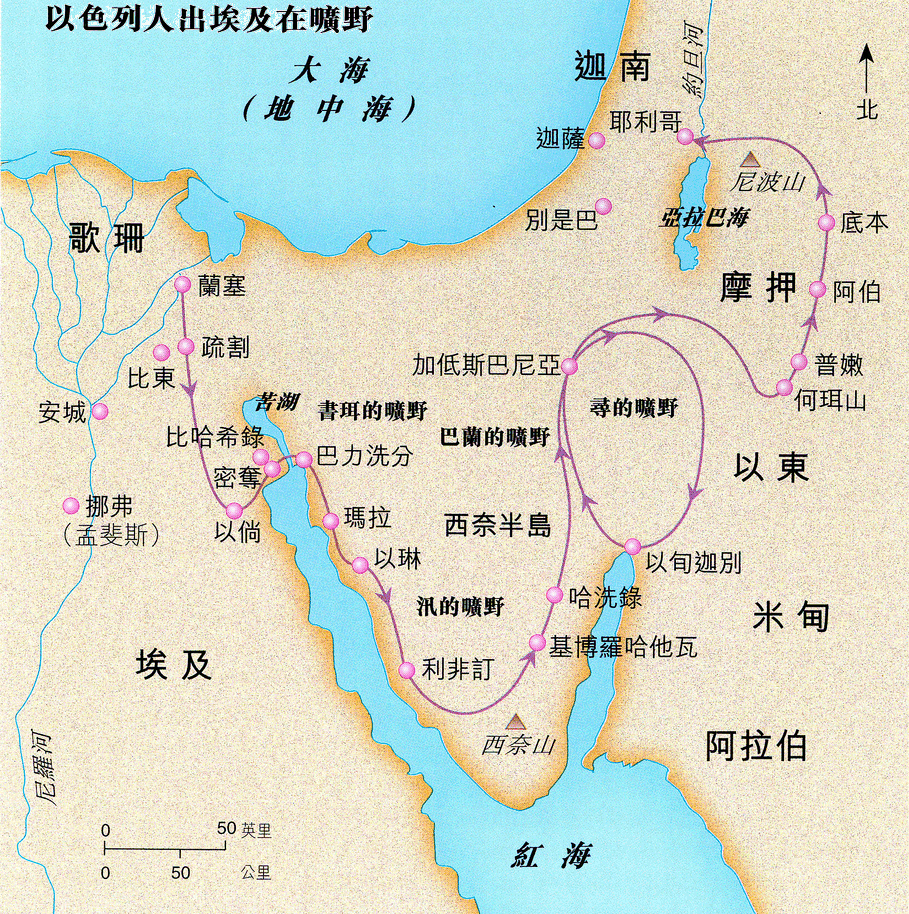
\includegraphics[width=5in]{AMoXiFigs/chuaiji/Exodus}
%\caption{以色列在曠野的經歷}
\label{fig:sub1}
\end{figure}

\begin{figure}%{.5\linewidth}
\centering
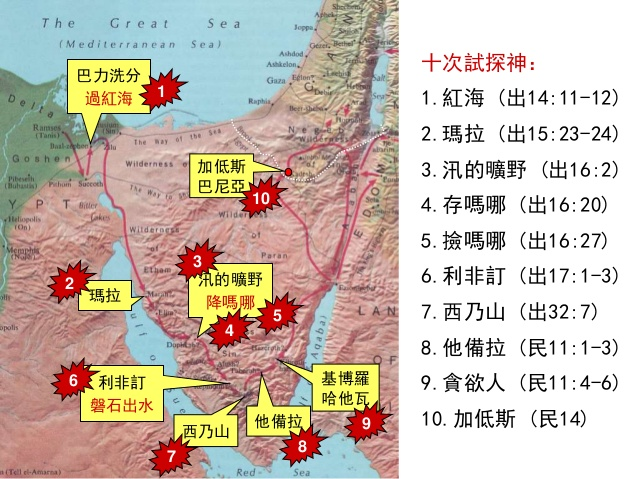
\includegraphics[width=6in]{AMoXiFigs/chuaiji/fig3}
%\caption{以色列在曠野的經歷}
\label{fig:sub1}
\end{figure}

\begin{figure}%{.5\linewidth}
\centering
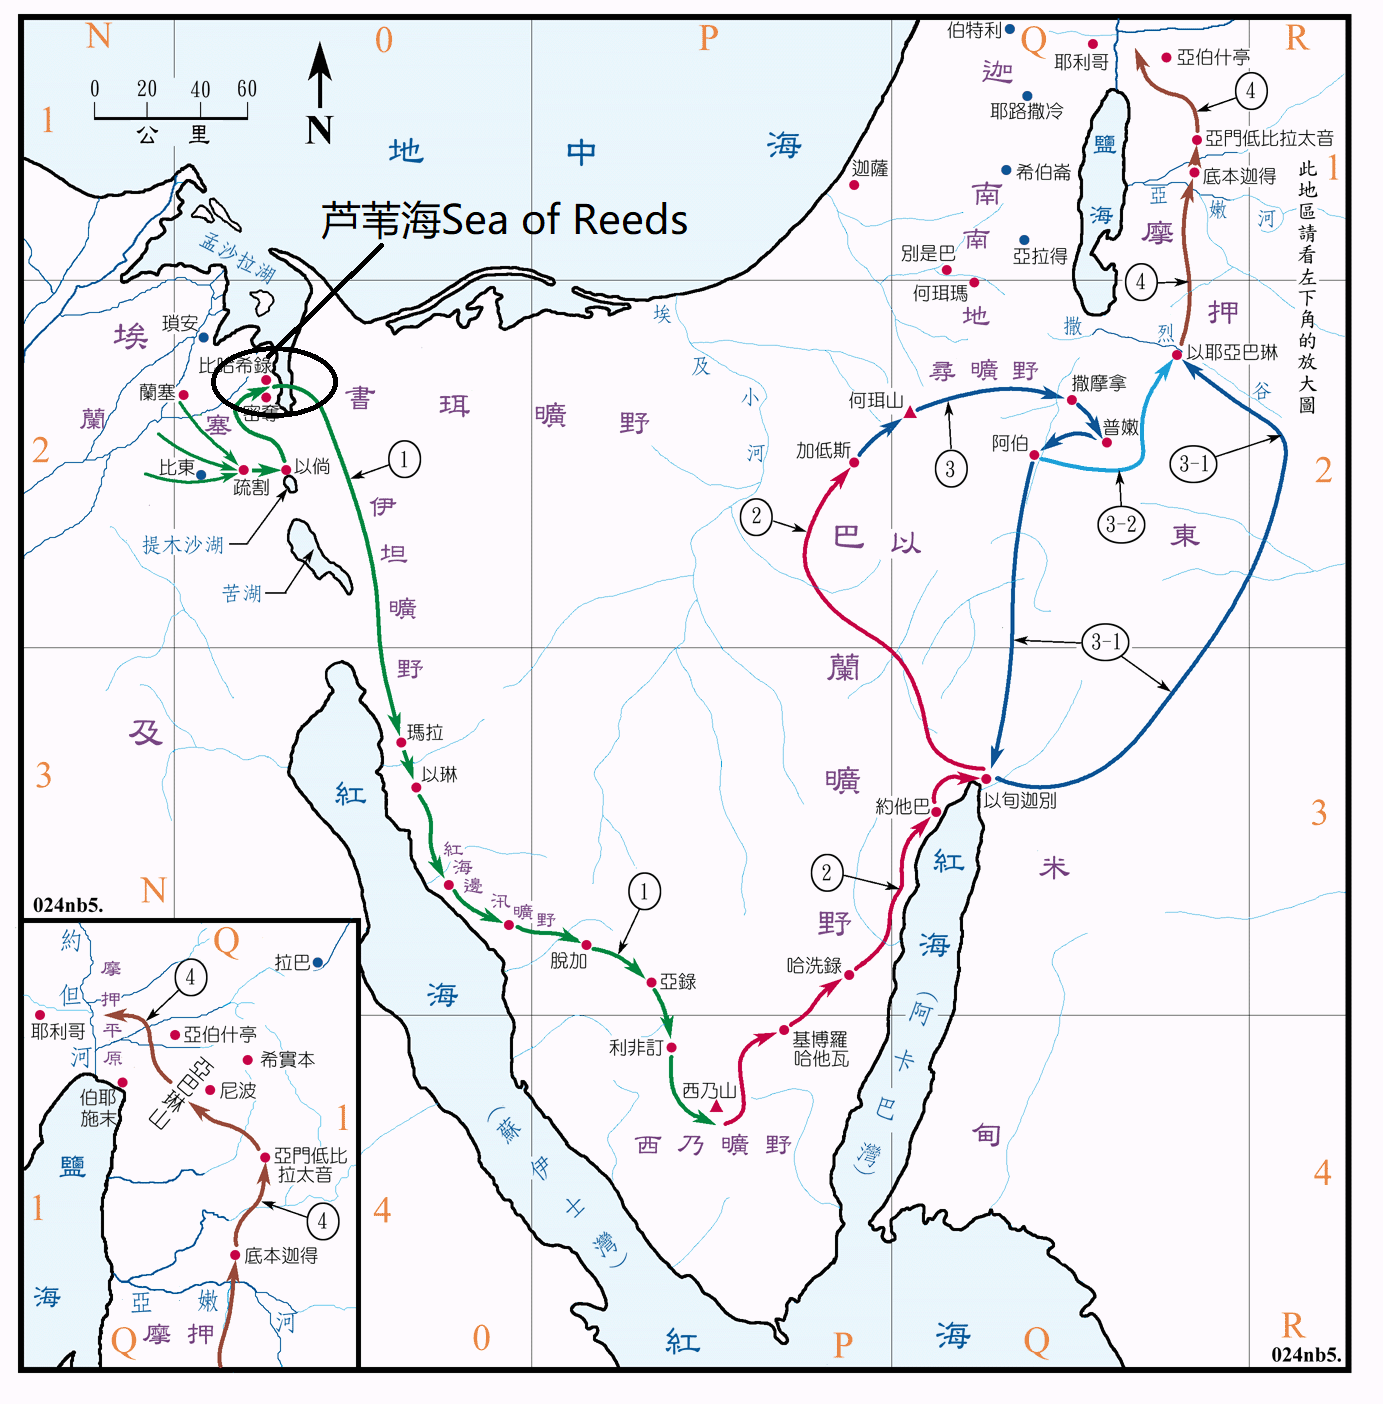
\includegraphics[width=6in]{AMoXiFigs/chuaiji/RedSee1}
%\caption{以色列在曠野的經歷}
\label{fig:sub1}
\end{figure}

\subsection{以色列人摆脱埃及軍隊 13:1-15:21}
\subsubsection{分別頭生 13:1-2(11-16)}
耶和華曉諭摩西說： 2 「以色列中凡頭生的，無論是人是牲畜，都是我的，要分別為聖歸我。」


\subsubsection{亞筆月向耶和華守無酵節七日 13:3-10}
摩西對百姓說：「你們要記念從埃及為奴之家出來的這日，因為耶和華用大能的手將你們從這地方領出來。有酵的餅都不可吃。 4 亞筆月間的這日是你們出來的日子。 5 將來耶和華領你進迦南人、赫人、亞摩利人、希未人、耶布斯人之地，就是他向你的祖宗起誓應許給你那流奶與蜜之地，那時你要在這月間守這禮。 6 你要吃無酵餅七日，到第七日要向耶和華守節。 7 這七日之久，要吃無酵餅，在你四境之內不可見有酵的餅，也不可見發酵的物。 8 當那日，你要告訴你的兒子說：『這是因耶和華在我出埃及的時候為我所行的事。』 9 這要在你手上做記號，在你額上做紀念，使耶和華的律法常在你口中，因為耶和華曾用大能的手將你從埃及領出來。 10 所以你每年要按著日期守這例。

\subsubsection{分別頭生公畜男婴 13:11-16}
將來，耶和華照他向你和你祖宗所起的誓將你領進迦南人之地，把這地賜給你， 12 那時你要將一切頭生的，並牲畜中頭生的，歸給耶和華，公的都要屬耶和華。 13 凡頭生的驢，你要用羊羔代贖，若不代贖，就要打折牠的頸項。凡你兒子中頭生的都要贖出來。 14 日後，你的兒子問你說：『這是什麼意思？』你就說：『耶和華用大能的手將我們從埃及為奴之家領出來。 15 那時法老幾乎不容我們去，耶和華就把埃及地所有頭生的，無論是人是牲畜，都殺了。因此，我把一切頭生的公牲畜獻給耶和華為祭，但將頭生的兒子都贖出來。 16 這要在你手上做記號，在你額上做經文，因為耶和華用大能的手將我們從埃及領出來。』」



\subsubsection{帶約瑟的骸骨繞道紅海曠野，日間雲柱和夜間火柱 13:17-22 }
17 法老容百姓去的時候，非利士地的道路雖近，神卻不領他們從那裡走，因為神說：「恐怕百姓遇見打仗後悔，就回埃及去。」 18 所以神領百姓繞道而行，走紅海曠野的路。以色列人出埃及地，都帶著兵器上去。 19 摩西把約瑟的骸骨一同帶去，因為約瑟曾叫以色列人嚴嚴地起誓，對他們說：「神必眷顧你們，你們要把我的骸骨從這裡一同帶上去。」 20 他們從疏割起行，在曠野邊的以倘安營。 21 日間耶和華在雲柱中領他們的路，夜間在火柱中光照他們，使他們日夜都可以行走。 22 日間雲柱，夜間火柱，總不離開百姓的面前。

%\vspace*{-\baselineskip}
\subsubsection{法老追襲以色列人 14:1-9}
耶和華曉諭摩西說： 2 「你吩咐以色列人轉回，安營在比哈希錄前、密奪和海的中間，對著巴力洗分，靠近海邊安營。 3 法老必說：『以色列人在地中繞迷了，曠野把他們困住了。』 4 我要使法老的心剛硬，他要追趕他們，我便在法老和他全軍身上得榮耀，埃及人就知道我是耶和華。」於是以色列人這樣行了。 5 有人告訴埃及王說：「百姓逃跑！」法老和他的臣僕就向百姓變心，說：「我們容以色列人去，不再服侍我們，這做的是什麼事呢？」 6 法老就預備他的車輛，帶領軍兵同去， 7 並帶著六百輛特選的車和埃及所有的車，每輛都有車兵長。 8 耶和華使埃及王法老的心剛硬，他就追趕以色列人，因為以色列人是昂然無懼地出埃及。 9 埃及人追趕他們，法老一切的馬匹、車輛、馬兵與軍兵就在海邊上，靠近比哈希錄，對著巴力洗分，在他們安營的地方追上了。

\begin{itemize} 
\itemsep-.35em 
\item 耶和華曉諭摩西說：「你\underline{吩咐以色列人轉回}，安營在比哈希錄前、密奪和海的中間，對著巴力洗分，靠近海邊安營。法老必說：『以色列人在地中繞迷了，曠野把他們困住了。』我要使法老的心剛硬，他要追趕他們，我便\underline{在法老和他全軍身上得榮耀，埃及人就知道我是耶和華}。」
\item 於是以色列人這樣行了。有人告訴埃及王說：「百姓逃跑！」法老和他的臣僕就向百姓變心，說：「我們容以色列人去，不再服侍我們，這做的是什麼事呢？」法老就預備他的車輛，帶領軍兵同去，並帶著六百輛特選的車和埃及所有的車，每輛都有車兵長。
\item 耶和華使埃及王法老的心剛硬，他就追趕以色列人，因為以色列人是昂然無懼地出埃及。埃及人追趕他們，法老一切的馬匹、車輛、馬兵與軍兵就在海邊上，靠近比哈希錄，對著巴力洗分，在他們安營的地方追上了。
\end{itemize}

\subsubsection{以色列人懼怕 14:10-14}
法老臨近的時候，以色列人舉目看見埃及人趕來，就甚懼怕，向耶和華哀求。 11 他們對摩西說：「難道在埃及沒有墳地，你把我們帶來死在曠野嗎？你為什麼這樣待我們，將我們從埃及領出來呢？ 12 我們在埃及豈沒有對你說過，不要攪擾我們，容我們服侍埃及人嗎？因為服侍埃及人比死在曠野還好。」 13 摩西對百姓說：「不要懼怕，只管站住，看耶和華今天向你們所要施行的救恩。因為你們今天所看見的埃及人，必永遠不再看見了。 14 耶和華必為你們爭戰，你們只管靜默，不要作聲。」

\begin{itemize} 
\itemsep-.35em 
\item 法老臨近的時候，以色列人舉目看見埃及人趕來，就甚懼怕，向耶和華哀求。他們對摩西說：「難道在埃及沒有墳地，你把我們帶來死在曠野嗎？你為什麼這樣待我們，將我們從埃及領出來呢？我們在埃及豈沒有對你說過，不要攪擾我們，容我們服侍埃及人嗎？因為服侍埃及人比死在曠野還好。」 
\item \underline{摩西對百姓說：「不要懼怕}，只管站住，看耶和華今天向你們所要施行的救恩。因為你們今天所看見的埃及人，必永遠不再看見了。耶和華必為你們爭戰，你們只管靜默，不要作聲。」
\end{itemize}

\subsubsection{紅海邊的雲柱拦阻埃及人 14:15-20}
耶和華對摩西說：「你為什麼向我哀求呢？你吩咐以色列人往前走。 16 你舉手向海伸杖，把水分開，以色列人要下海中走乾地。 17 我要使埃及人的心剛硬，他們就跟著下去，我要在法老和他的全軍、車輛、馬兵上得榮耀。 18 我在法老和他的車輛、馬兵上得榮耀的時候，埃及人就知道我是耶和華了。」 19 在以色列營前行走神的使者，轉到他們後邊去，雲柱也從他們前邊轉到他們後邊立住。 20 在埃及營和以色列營中間有雲柱，一邊黑暗，一邊發光，終夜兩下不得相近。

\begin{itemize} 
\itemsep-.35em 
\item 耶和華對摩西說：「你為什麼向我哀求呢？你吩咐以色列人往前走。你舉手向海伸杖，把水分開，以色列人要下海中走乾地。我要使埃及人的心剛硬，他們就跟著下去，我要在法老和他的全軍、車輛、馬兵上得榮耀。我在法老和他的車輛、馬兵上得榮耀的時候，埃及人就知道我是耶和華了。」 
\item 在以色列營前行走神的使者，轉到他們後邊去，雲柱也從他們前邊轉到他們後邊立住。在埃及營和以色列營中間有雲柱，一邊黑暗，一邊發光，終夜兩下不得相近
\end{itemize}

\subsubsection{投埃及人於海 14:21-31}
摩西向海伸杖，耶和華便用大東風使海水一夜退去，水便分開，海就成了乾地。 22 以色列人下海中走乾地，水在他們的左右做了牆垣。 23 埃及人追趕他們，法老一切的馬匹、車輛和馬兵都跟著下到海中。 24 到了晨更的時候，耶和華從雲火柱中向埃及的軍兵觀看，使埃及的軍兵混亂了， 25 又使他們的車輪脫落，難以行走，以致埃及人說：「我們從以色列人面前逃跑吧！因耶和華為他們攻擊我們了。」

耶和華對摩西說：「你向海伸杖，叫水仍合在埃及人並他們的車輛、馬兵身上。」 27 摩西就向海伸杖，到了天一亮，海水仍舊復原。埃及人避水逃跑的時候，耶和華把他們推翻在海中， 28 水就回流，淹沒了車輛和馬兵。那些跟著以色列人下海法老的全軍，連一個也沒有剩下。 29 以色列人卻在海中走乾地，水在他們的左右做了牆垣。 30 當日，耶和華這樣拯救以色列人脫離埃及人的手，以色列人看見埃及人的死屍都在海邊了。 31 以色列人看見耶和華向埃及人所行的大事，就敬畏耶和華，又信服他和他的僕人摩西。

\begin{itemize} 
\itemsep-.35em 
\item 摩西向海伸杖，耶和華便用\underline{大東風使海水一夜退去，水便分開，海就成了乾地}。
\begin{itemize} 
\itemsep-.35em 
\item 以色列人下海中走乾地，水在他們的左右做了牆垣。 
\item 埃及人追趕他們，法老一切的馬匹、車輛和馬兵都跟著下到海中。
\item 到了晨更的時候，耶和華\underline{從雲火柱中向埃及的軍兵觀看}，使埃及的軍兵混亂了，又使他們的車輪脫落，難以行走，以致埃及人說：「我們從以色列人面前逃跑吧！因耶和華為他們攻擊我們了。」
\end{itemize}
\item 耶和華對摩西說：「你向海伸杖，叫水仍合在埃及人並他們的車輛、馬兵身上。」摩西就向海伸杖，到了天一亮，\underline{海水仍舊復原}。 
\begin{itemize} 
\itemsep-.35em 
\item 埃及人避水逃跑的時候，耶和華把他們推翻在海中，水就回流，淹沒了車輛和馬兵。那些跟著以色列人下海法老的全軍，連一個也沒有剩下。
\item 以色列人卻在海中走乾地，水在他們的左右做了牆垣。當日，耶和華這樣拯救以色列人脫離埃及人的手,以色列人看見埃及人的死屍都在海邊了。以色列人看見耶和華向埃及人所行的大事，就敬畏耶和華，又信服他和他的僕人摩西。
\end{itemize}
\end{itemize}

\subsubsection{摩西歌頌耶和華 15:1-18}
\begin{itemize} 
\itemsep-.35em 
\item 那時，摩西和以色列人向耶和華\underline{唱歌}說：我要向耶和華歌唱,因他大大戰勝，將馬和騎馬的投在海中。耶和華是我的力量、我的詩歌，也成了我的拯救。這是我的神，我要讚美他；是我父親的神，我要尊崇他。耶和華是戰士，他的名是耶和華。\underline{法老}的車輛、軍兵，耶和華已拋在海中，他特選的軍長都沉於紅海。深水淹沒他們，他們如同石頭墜到深處。 耶和華啊，你的右手施展能力，顯出榮耀；耶和華啊，你的右手摔碎仇敵。你大發威嚴，推翻那些起來攻擊你的；你發出烈怒如火，燒滅他們像燒碎秸一樣。你發鼻中的氣，水便聚起成堆，大水直立如壘，海中的深水凝結。仇敵說：『我要追趕，我要追上；我要分擄物；我要在他們身上稱我的心願；我要拔出刀來，親手殺滅他們。』你叫風一吹，海就把他們淹沒，他們如鉛沉在大水之中。 
\item 耶和華啊，眾神之中誰能像你？誰能像你至聖至榮，可頌可畏，施行奇事？你伸出右手，地便吞滅他們。你憑慈愛領了你所贖的百姓，你憑能力引他們到了你的聖所。\underline{外邦人}聽見就發顫，疼痛抓住\underline{非利士}的居民。那時，\underline{以東}的族長驚惶，\underline{摩押}的英雄被戰兢抓住，\underline{迦南}的居民心都消化了，驚駭恐懼臨到他們。耶和華啊，因你膀臂的大能，他們如石頭寂然不動，等候你的百姓過去，等候你所贖的百姓過去。你要將他們領進去，栽於你產業的山上。耶和華啊，就是你為自己所造的住處；主啊，就是你手所建立的聖所。耶和華必做王，直到永永遠遠。」
\end{itemize}

\subsubsection{米利暗歌頌耶和華 15:19-21}
\begin{itemize} 
\itemsep-.35em
\item 法老的馬匹、車輛和馬兵下到海中，耶和華使海水回流淹沒他們，唯有以色列人在海中走乾地。 
\item 亞倫的姐姐女先知米利暗，手裡拿著鼓，眾婦女也跟她出去拿鼓跳舞。
\item 米利暗應聲說：「你們要歌頌耶和華，因他大大戰勝，將馬和騎馬的投在海中。」
\end{itemize}

\subsection{以色列人在曠野 15:22-18:27}
\subsubsection{在瑪拉因為水苦發怨言,樹使苦水變甜 15:22-26}
\begin{itemize} 
\itemsep-.35em
\item 摩西領以色列人從紅海往前行，到了書珥的曠野，在曠野走了三天，找不著水。到了瑪拉，不能喝那裡的水，因為水苦，所以那地名叫瑪拉。 
\item 百姓就向摩西發怨言，說：「我們喝什麼呢？」摩西呼求耶和華，耶和華指示他一棵樹。他把樹丟在水裡，水就變甜了。
\item 耶和華在那裡為他們定了律例、典章，在那裡試驗他們。又說：「你若留意聽耶和華你神的話，又行我眼中看為正的事，留心聽我的誡命，守我一切的律例，我就不將所加於埃及人的疾病加在你身上，因為我耶和華是醫治你的。」
\end{itemize}

\subsubsection{在以琳遇水泉十二 15:27}
\begin{itemize} 
\itemsep-.35em
\item 他們到了以琳，在那裡有十二股水泉，七十棵棕樹，
\item 他們就在那裡的水邊安營。
\end{itemize}

\subsubsection{汛的曠野因饥饿發怨言 16:1-3}
\begin{itemize} 
\itemsep-.35em
\item 以色列全會眾從以琳起行，在出埃及後第二個月十五日，到了以琳和西奈中間汛的曠野。
\item 以色列全會眾在曠野向摩西、亞倫發怨言，說：「巴不得我們早死在埃及地耶和華的手下，那時我們坐在肉鍋旁邊，吃得飽足。你們將我們領出來，到這曠野，是要叫這全會眾都餓死啊！」
\end{itemize}

\subsubsection{神应许賜鵪鶉和嗎哪 16:4-12}
\begin{itemize} 
\itemsep-.35em
\item 耶和華對摩西說：「我要將糧食從天降給你們。百姓可以出去，每天收每天的份，我好試驗他們遵不遵我的法度。到第六天，他們要把所收進來的預備好了，比每天所收的多一倍。」 摩西、亞倫對以色列眾人說：
\begin{itemize} 
\itemsep-.35em
\item 「到了晚上，你們要知道是耶和華將你們從埃及地領出來的。早晨，你們要看見耶和華的榮耀，因為耶和華聽見你們向他所發的怨言了。我們算什麼，你們竟向我們發怨言呢？」 
\item 摩西又說：「耶和華晚上必給你們肉吃，早晨必給你們食物得飽，因為你們向耶和華發的怨言，他都聽見了。我們算什麼？你們的怨言不是向我們發的，乃是向耶和華發的。」 
\item 摩西對亞倫說：「你告訴以色列全會眾說：『你們就近耶和華面前，因為他已經聽見你們的怨言了。』」 
\end{itemize}
\item 亞倫正對以色列全會眾說話的時候，他們向曠野觀看，不料，耶和華的榮光在雲中顯現。耶和華曉諭摩西說：「我已經聽見以色列人的怨言。你告訴他們說：『到黃昏的時候，你們要吃肉，早晨必有食物得飽，你們就知道我是耶和華你們的神。』」
\end{itemize}

\subsubsection{晚上賜鵪鶉，早晨降嗎哪 16:13-15}
\begin{itemize} 
\itemsep-.35em
\item 到了晚上，有\underline{鵪鶉}飛來，遮滿了營。
\item 早晨，在營四圍的地上有露水。露水上升之後，不料，野地面上有\underline{如白霜的小圓物}。
\item 以色列人看見不知道是什麼，就彼此對問說：「這是什麼呢？」摩西對他們說：「這就是耶和華給你們吃的食物
\end{itemize}

\subsubsection{收取嗎哪之例 16:16-30}
\begin{itemize} 
\itemsep-.35em
\item 耶和華所吩咐的是這樣：你們要按著各人的飯量，為帳篷裡的人按著人數收起來，各拿一俄梅珥。
\begin{itemize} 
\itemsep-.35em
\item 以色列人就這樣行，有多收的，有少收的。及至用俄梅珥量一量，多收的也沒有餘，少收的也沒有缺，各人\underline{按著自己的飯量收取}。 
\item 摩西對他們說：「所收的，\underline{不許什麼人留到早晨}。」然而他們不聽摩西的話，內中有留到早晨的，就生蟲變臭了。摩西便向他們發怒。
\end{itemize}
\item 他們每日早晨，按著各人的飯量收取，\underline{日頭一發熱就消化了}。 22 到\underline{第六天}，他們收了\underline{雙倍的食物}，每人兩俄梅珥。會眾的官長來告訴摩西， 23 摩西對他們說：「耶和華這樣說：『明天是聖安息日，是向耶和華守的聖安息日。你們要烤的就烤了，要煮的就煮了，所剩下的都留到早晨。』」
\item 他們就照摩西的吩咐留到早晨，也不臭，裡頭也沒有蟲子。 25 摩西說：「你們今天吃這個吧，因為今天是向耶和華守的安息日，你們在田野必找不著了。 26 六天可以收取，第七天乃是安息日，那一天必沒有了。」 
\item 第七天，百姓中有人出去收，什麼也找不著。耶和華對摩西說：「你們不肯守我的誡命和律法，要到幾時呢？ 29 你們看，耶和華既將安息日賜給你們，所以第六天他賜給你們兩天的食物，第七天各人要住在自己的地方，不許什麼人出去。」 於是百姓第七天安息了。
\end{itemize}

\subsubsection{嗎哪 16:31-36}
\begin{itemize} 
\itemsep-.35em
\item 這食物，以色列家叫嗎哪，樣子像芫荽子，顏色是白的，滋味如同攙蜜的薄餅。
\item 摩西說：「耶和華所吩咐的是這樣：要將一滿俄梅珥嗎哪留到世世代代，使後人可以看見我當日將你們領出埃及地，在曠野所給你們吃的食物。」摩西對亞倫說：「你拿一個罐子，盛一滿俄梅珥嗎哪，存在耶和華面前，要留到世世代代。」
\item 耶和華怎麼吩咐摩西，亞倫就怎麼行，把嗎哪放在法櫃前存留。以色列人吃嗎哪共四十年，直到進了有人居住之地，就是迦南的境界。（俄梅珥乃伊法十分之一。）
\end{itemize}

\subsubsection{米利巴摩西擊打磐石 17:1-7 (民數記20:1-13)}
\begin{itemize} 
\itemsep-.35em
\item 以色列全會眾都遵耶和華的吩咐，按著站口從汛的曠野往前行，在利非訂安營。
百姓沒有水喝，所以與摩西爭鬧，說：「給我們水喝吧！」摩西對他們說：「你們為什麼與我爭鬧，為什麼試探耶和華呢？」百姓在那裡甚渴，要喝水，就向摩西發怨言，說：「你為什麼將我們從埃及領出來，使我們和我們的兒女並牲畜都渴死呢？」 
\item 摩西就呼求耶和華說：「我向這百姓怎樣行呢？他們幾乎要拿石頭打死我。」耶和華對摩西說：「你手裡拿著你先前擊打河水的杖，帶領以色列的幾個長老，從百姓面前走過去。我必在何烈的磐石那裡，站在你面前。你要擊打磐石，從磐石裡必有水流出來，使百姓可以喝。」
\item 摩西就在以色列的長老眼前這樣行了。 
\begin{itemize} 
\itemsep-.35em
\item 他給那地方起名叫瑪撒 (試探)，
\item 又叫米利巴(爭鬧)，因以色列人爭鬧，又因他們試探耶和華，說：「耶和華是在我們中間不是？」
\end{itemize}
\end{itemize}

\subsubsection{與亞瑪力人爭戰 17:8-16 }
\begin{itemize} 
\itemsep-.35em
\item 那時，亞瑪力人來在利非訂，和以色列人爭戰。摩西對約書亞說：「你為我們選出人來，出去和亞瑪力人爭戰。明天我手裡要拿著神的杖，站在山頂上。」 
\begin{itemize} 
\itemsep-.35em
\item 於是約書亞照著摩西對他所說的話行，和亞瑪力人爭戰。
\item 摩西、亞倫與戶珥都上了山頂。摩西何時舉手，以色列人就得勝；何時垂手，亞瑪力人就得勝。但摩西的手發沉，他們就搬石頭來，放在他以下，他就坐在上面。亞倫與戶珥扶著他的手，一個在這邊，一個在那邊，他的手就穩住，直到日落的時候。
\item 約書亞用刀殺了亞瑪力王和他的百姓。 
\end{itemize}
\item 耶和華對摩西說：「我要將亞瑪力的名號從天下全然塗抹了，你要將這話寫在書上做紀念，又念給約書亞聽。」摩西築了一座壇，起名叫耶和華尼西 (耶和華是我旌旗)，又說：「耶和華已經起了誓，必世世代代和亞瑪力人爭戰。」
\end{itemize}

\subsubsection{摩西的岳父葉忒羅稱頌神 18:1-13 }
\begin{itemize} 
\itemsep-.35em
\item 摩西的岳父米甸祭司葉忒羅，聽見神為摩西和神的百姓以色列所行的一切事，就是耶和華將以色列從埃及領出來的事，便帶著摩西的妻子西坡拉，就是摩西從前打發回去的，又帶著西坡拉的兩個兒子，一個名叫革舜，因為摩西說：「我在外邦做了寄居的」，一個名叫以利以謝，因為他說：「我父親的神幫助了我，救我脫離法老的刀」——摩西的岳父葉忒羅帶著摩西的妻子和兩個兒子來到神的山，就是摩西在曠野安營的地方。
\item 他對摩西說：「我是你岳父葉忒羅，帶著你的妻子和兩個兒子來到你這裡。」摩西迎接他的岳父，向他下拜，與他親嘴，彼此問安，都進了帳篷。摩西將耶和華為以色列的緣故向法老和埃及人所行的一切事，以及路上所遭遇的一切艱難，並耶和華怎樣搭救他們，都述說於他岳父聽。
\item 葉忒羅因耶和華待以色列的一切好處，就是拯救他們脫離埃及人的手，便甚歡喜。
\begin{itemize} 
\itemsep-.35em
\item 葉忒羅說：「耶和華是應當稱頌的！他救了你們脫離埃及人和法老的手，將這百姓從埃及人的手下救出來。我現今在埃及人向這百姓發狂傲的事上得知，耶和華比萬神都大。」
\item 摩西的岳父葉忒羅把燔祭和平安祭獻給神。亞倫和以色列的眾長老都來了，與摩西的岳父在神面前吃飯
\end{itemize}
\end{itemize}

\subsubsection{葉忒羅獻策選立百姓官長 18:13-27 (申命記1:9-18)}
\begin{itemize} 
\itemsep-.35em
\item 第二天，摩西坐著審判百姓，百姓從早到晚都站在摩西的左右。
\begin{itemize} 
\itemsep-.35em
\item 摩西的岳父看見他向百姓所做的一切事，就說：「你向百姓做的是什麼事呢？你為什麼獨自坐著，眾百姓從早到晚都站在你的左右呢？」
\item 摩西對岳父說：「這是因百姓到我這裡來求問神。他們有事的時候就到我這裡來，我便在兩造之間施行審判，我又叫他們知道神的律例和法度。」 
\end{itemize}
\item 摩西的岳父說：「你這做的不好。你和這些百姓必都疲憊，因為這事太重，你獨自一人辦理不了。 現在你要聽我的話，我為你出個主意，願神與你同在。
\begin{itemize} 
\itemsep-.35em
\item 你要替百姓到神面前，將案件奏告神。又要將律例和法度教訓他們，指示他們當行的道、當做的事。
\item 並要從百姓中揀選有才能的人，就是敬畏神、誠實無妄、恨不義之財的人，派他們做千夫長、百夫長、五十夫長、十夫長，管理百姓。叫他們隨時審判百姓，大事都要呈到你這裡，小事他們自己可以審判
\item 這樣，你就輕省些，他們也可以同當此任。你若這樣行，神也這樣吩咐你，你就能受得住，這百姓也都平平安安歸回他們的住處。」 
\end{itemize}
\item 於是，摩西聽從他岳父的話，按著他所說的去行。摩西從以色列人中揀選了有才能的人，立他們為百姓的首領，做千夫長、百夫長、五十夫長、十夫長。他們隨時審判百姓，有難斷的案件就呈到摩西那裡，但各樣小事他們自己審判。此後，摩西讓他的岳父去，他就往本地去了
\end{itemize}

\section{西奈山得律法，建会幕和祭司体制 19-40}
\subsection{摩西一次上山得十誡 19:1-20:21}
\subsubsection{以色列人至西奈山 19:1-15 }
\begin{itemize} 
\itemsep-.35em
\item 以色列人出埃及地以後，滿了三個月的那一天，就來到西奈的曠野。他們離了利非訂，來到西奈的曠野，就在那裡的山下安營。摩西到神那裡，
\begin{table}[H]
\begin{threeparttable}
\begin{tabular}{@{}p{0.65\textwidth}*{4}{L{\dimexpr0.41\linewidth-10\tabcolsep\relax}}@{}}
\toprule
神 &  摩西 \\\hline
耶和華從山上呼喚他說：「你要這樣告訴雅各家，曉諭以色列人說：我向埃及人所行的事，你們都看見了；且看見我如鷹將你們背在翅膀上，帶來歸我。如今你們若實在聽從我的話，遵守我的約，就要在萬民中做屬我的子民，因為全地都是我的。你們要歸我做祭司的國度，為聖潔的國民。這些話你要告訴以色列人。」 &摩西去召了民間的長老來，將耶和華所吩咐他的話都在他們面前陳明。百姓都同聲回答說：「凡耶和華所說的，我們都要遵行。」摩西就將百姓的話回覆耶和華\tabularnewline\hline
耶和華對摩西說：「我要在密雲中臨到你那裡，叫百姓在我與你說話的時候可以聽見，也可以永遠信你了。」&於是，摩西將百姓的話奏告耶和華  \tabularnewline\hline
耶和華又對摩西說：「你往百姓那裡去，叫他們今天、明天自潔，又叫他們洗衣服。到第三天要預備好了，因為第三天耶和華要在眾百姓眼前降臨在西奈山上。你要在山的四圍給百姓定界限，說：『你們當謹慎，不可上山去，也不可摸山的邊界。凡摸這山的，必要治死他——不可用手摸他，必用石頭打死，或用箭射透。無論是人是牲畜，都不得活。到角聲拖長的時候，他們才可到山根來。』」&摩西下山往百姓那裡去，叫他們自潔，他們就洗衣服。他對百姓說：「到第三天要預備好了。不可親近女人。」 \tabularnewline
\hline
\bottomrule
\end{tabular}
\caption{百姓自潔豫備見神}
\end{threeparttable}
\end{table} 
\end{itemize}

\subsubsection{耶和華於火中降臨西奈山 19:16-25}
\begin{itemize} 
\itemsep-.35em
\item 到了第三天早晨
\begin{itemize} 
\itemsep-.35em
\item 在\underline{山上}有雷轟、閃電和密雲，並且角聲甚大
\item \underline{營中}的百姓盡都發顫。摩西率領百姓出營迎接神，都站在山下
\item 西奈\underline{全山}冒煙，因為耶和華在火中降於山上。山的煙氣上騰，如燒窯一般，遍山大大地震動。角聲漸漸地高而又高
\end{itemize}
\item 摩西就說話，神有聲音答應他。耶和華降臨在西奈山頂上，耶和華召摩西上山頂，摩西就上去。
\begin{table}[H]
\begin{threeparttable}
\begin{tabular}{@{}p{0.6\textwidth}*{4}{L{\dimexpr0.45\linewidth-10\tabcolsep\relax}}@{}}
\toprule
神 &  摩西 \\\hline
耶和華對摩西說：「你下去囑咐百姓，不可闖過來到我面前觀看，恐怕他們有多人死亡。又叫親近我的祭司自潔，恐怕我忽然出來擊殺他們。」&摩西對耶和華說：「百姓不能上西奈山，因為你已經囑咐我們說：『要在山的四圍定界限，叫山成聖。』」\tabularnewline\hline
耶和華對他說：「下去吧，你要和亞倫一同上來，只是祭司和百姓不可闖過來上到我面前，恐怕我忽然出來擊殺他們。」&於是摩西下到百姓那裡告訴他們。 \tabularnewline\hline
\hline
\bottomrule
\end{tabular}
\caption{耶和華於火中降臨西奈山}
\end{threeparttable}
\end{table} 
\end{itemize}


\subsubsection{頒布十誡 20:1-17 (申5:6-21)}
\begin{itemize} 
\itemsep-.35em
\item 对神的条例
\begin{itemize} 
\itemsep-.35em
\item 神吩咐這一切的話說：「我是耶和華你的神，曾將你從埃及地為奴之家領出來。除了我以外，你\underline{不可有別的神}
\item \underline{不可為自己雕刻偶像}，也不可做什麼形象彷彿上天、下地和地底下、水中的百物。不可跪拜那些像，也不可侍奉它，因為我耶和華你的神是忌邪的神。恨我的，我必追討他的罪，自父及子，直到三四代；愛我守我誡命的，我必向他們發慈愛，直到千代
\item \underline{不可妄稱耶和華你神的名}，因為妄稱耶和華名的，耶和華必不以他為無罪
\item \underline{當記念安息日}，守為聖日。六日要勞碌做你一切的工，但第七日是向耶和華你神當守的安息日。這一日你和你的兒女、僕婢、牲畜，並你城裡寄居的客旅，無論何工都不可做。因為六日之內，耶和華造天、地、海和其中的萬物，第七日便安息，所以耶和華賜福於安息日，定為聖日
\end{itemize}
\item 对人的条例
\begin{itemize} 
\itemsep-.35em
\item \underline{當}孝敬父母，使你的日子在耶和華你神所賜你的地上得以長久
\item \underline{不可}殺人
\item \underline{不可}姦淫
\item \underline{不可}偷盜
\item \underline{不可}作假見證陷害人
\item \underline{不可}貪戀人的房屋，也不可貪戀人的妻子、僕婢、牛驢並他一切所有的。
\end{itemize}
\end{itemize}


\subsubsection{百姓見神而懼怕 20:18-21 (申命記5:23-27)}
\begin{itemize} 
\itemsep-.35em
\item 眾百姓見雷轟、閃電、角聲、山上冒煙，就都發顫，遠遠地站立，對摩西說：「求你和我們說話，我們必聽；不要神和我們說話，恐怕我們死亡。」 
\item 摩西對百姓說：「不要懼怕，因為神降臨是要試驗你們，叫你們時常敬畏他，不致犯罪。」於是百姓遠遠地站立，摩西就挨近神所在的幽暗之中。
\end{itemize}


\subsection{摩西二次上山得律法 20:22-23:33}
\subsubsection{禁造神像和築（土、石）壇之條例 20:22-26}
\begin{itemize} 
\itemsep-.35em
\item 耶和華對摩西說：「你要向以色列人這樣說：你們自己看見我從天上和你們說話了。你們\underline{不可做什麼神}像與我相配，不可為自己做金銀的神像。
\item 你要為我\underline{築土壇}，在上面以牛羊獻為燔祭和平安祭。凡記下我名的地方，我必到那裡賜福給你。
 \item 你若為我\underline{築一座石壇}，不可用鑿成的石頭，因你在上頭一動家具，就把壇汙穢了。
\item 你上我的壇，\underline{不可用臺階}，免得露出你的下體來。
\end{itemize}


\subsubsection{對待奴僕之例 21:1-11 （申15:12-18/利25:39-55）}
\begin{itemize} 
\itemsep-.35em
\item 男僕：你在百姓面前所要立的典章是這樣：你若買希伯來人做奴僕
\begin{itemize} 
\itemsep-.35em
\item 他必服侍你六年，第七年他可以自由，白白地出去。
\begin{itemize} 
\itemsep-.35em
\item 他若孤身來，就可以孤身去；
\item 他若有妻，他的妻就可以同他出去。
\item 他主人若給他妻子，妻子給他生了兒子或女兒，妻子和兒女要歸主人，他要獨自出去。
\end{itemize}
\item 倘或奴僕明說：『我愛我的主人和我的妻子、兒女，不願意自由出去。』他的主人就要帶他到審判官（神）那裡，又要帶他到門前，靠近門框，用錐子穿他的耳朵，他就永遠服侍主人。
\end{itemize}
\item 女僕：人若賣女兒做婢女，婢女不可像男僕那樣出去。
\begin{itemize} 
\itemsep-.35em
\item 主人選定她歸自己，若不喜歡她，就要許她贖身；主人既然用詭詐待她，就沒有權柄賣給外邦人。
\item 主人若選定她給自己的兒子，就當待她如同女兒。若另娶一個，那女子的吃食、衣服並好合的事，仍不可減少。若不向她行這三樣，她就可以不用錢贖，白白地出去。
\end{itemize}
\end{itemize}

\subsubsection{人傷害人的赔偿條例 21:12-27}
\begin{itemize} 
\itemsep-.35em
\item 人若彼此相爭
\begin{itemize} 
\itemsep-.35em
\item 打人以致打死的，必要把他治死。人若不是埋伏著殺人，乃是神交在他手中，我就設下一個地方，他可以往那裡逃跑。人若任意用詭計殺了他的鄰舍，就是逃到我的壇那裡，也當捉去把他治死。
\item 人若彼此相爭，這個用石頭或是拳頭打那個，尚且不至於死，不過躺臥在床，若再能起來扶杖而出，那打他的可算無罪，但要將他耽誤的工夫用錢賠補，並要將他全然醫好。
\item 人若彼此爭鬥，傷害有孕的婦人，甚至墜胎，隨後卻無別害，那傷害她的總要按婦人的丈夫所要的，照審判官所斷的受罰。若有別害，就要以命償命，以眼還眼，以牙還牙，以手還手，以腳還腳，以烙還烙，以傷還傷，以打還打。
\end{itemize}
\item 拐帶人口，或是把人賣了，或是留在他手下，必要把他治死。
\item 人若与父母相爭
\begin{itemize} 
\itemsep-.35em
\item 打父母的，必要把他治死。
\item 咒罵父母的，必要把他治死。
\end{itemize}
\item 打死打壞奴僕
\begin{itemize} 
\itemsep-.35em
\item 人若用棍子打奴僕或婢女，立時死在他的手下，他必要受刑。若過一兩天才死，就可以不受刑，因為是用錢買的。
\item 人若打壞了他奴僕或是婢女的一隻眼，就要因他的眼放他去得以自由。若打掉了他奴僕或是婢女的一個牙，就要因他的牙放他去得以自由。
\end{itemize}
\end{itemize}

\subsubsection{人傷動物或動物傷人的條例 21:28-36}
\begin{itemize} 
\itemsep-.35em
\item 牛若觸死男人或是女人
\begin{itemize} 
\itemsep-.35em
\item 牛若觸了自由人
\begin{itemize} 
\itemsep-.35em
\item 總要用石頭打死那牛，卻不可吃牠的肉，牛的主人可算無罪。
\item 倘若那牛素來是觸人的，有人報告了牛主，他竟不把牛拴著，以致把男人或是女人觸死，就要用石頭打死那牛，牛主也必治死。
\item 若罰他贖命的價銀，他必照所罰的贖他的命。
\item 牛無論觸了人的兒子或是女兒，必照這例辦理。
\end{itemize}
\item 牛若觸了奴僕或是婢女，必將銀子三十舍客勒給他們的主人，也要用石頭把牛打死。
\end{itemize}
\item 人若敞著井口，或挖井不遮蓋，有牛或驢掉在裡頭，井主要拿錢賠還本主人，死牲畜要歸自己
\item 牛傷牛
\begin{itemize} 
\itemsep-.35em
\item 這人的牛若傷了那人的牛，以至於死，他們要賣了活牛，平分價值，也要平分死牛。 \item 人若知道這牛素來是觸人的，主人竟不把牛拴著，他必要以牛還牛，死牛要歸自己
\end{itemize}
\end{itemize}

\subsubsection{賠償的條例 22:1-17}
\begin{itemize} 
\itemsep-.35em
\item 牲畜造成的损失
\begin{itemize} 
\itemsep-.35em
\item 人若偷牛或羊，無論是宰了是賣了，他就要以五牛賠一牛，四羊賠一羊。
\item 人若遇見賊挖窟窿，把賊打了，以至於死，就不能為他有流血的罪。若太陽已經出來，就為他有流血的罪。
\item 賊若被拿，總要賠還。若他一無所有，就要被賣，頂他所偷的物。若他所偷的，或牛，或驢，或羊，仍在他手下存活，他就要加倍賠還。
\item 人若在田間或在葡萄園裡放牲畜，任憑牲畜上別人的田裡去吃，就必拿自己田間上好的和葡萄園上好的賠還。
\end{itemize}
\item 人为造成的损失
\begin{itemize} 
\itemsep-.35em
\item 若點火焚燒荊棘，以致將別人堆積的禾捆、站著的禾稼或是田園，都燒盡了，那點火的必要賠還。
\item 人若將銀錢或家具交付鄰舍看守，這物從那人的家被偷去，若把賊找到了，賊要加倍賠還。若找不到賊，那家主必就近審判官，要看看他拿了原主的物件沒有。兩個人的案件，無論是為什麼過犯，或是為牛，為驢，為羊，為衣裳，或是為什麼失掉之物，有一人說『這是我的』，兩造就要將案件稟告審判官，審判官定誰有罪，誰就要加倍賠還。
\item 人若將驢，或牛，或羊，或別的牲畜，交付鄰舍看守，牲畜或死，或受傷，或被趕去，無人看見，那看守的人要憑著耶和華起誓，手裡未曾拿鄰舍的物，本主就要罷休，看守的人不必賠還。牲畜若從看守的那裡被偷去，他就要賠還本主。若被野獸撕碎，看守的要帶來當做證據，所撕的不必賠還。
\item 人若向鄰舍借什麼，所借的或受傷，或死，本主沒有同在一處，借的人總要賠還。若本主同在一處，他就不必賠還。若是雇的，也不必賠還，本是為雇價來的。
\item 人若引誘沒有受聘的處女，與她行淫，他總要交出聘禮，娶她為妻。若女子的父親決不肯將女子給他，他就要按處女的聘禮，交出錢來。
\end{itemize}
\end{itemize}

\subsubsection{敬畏神和不可虧負弱者的條例 22:18-31}
\begin{itemize} 
\itemsep-.35em
\item 敬畏神的条例
\begin{itemize} 
\itemsep-.35em
\item 行邪術的女人，不可容她存活。
\item 凡與獸淫合的，總要把他治死。
\item 祭祀別神，不單單祭祀耶和華的，那人必要滅絕。
\item 不可毀謗神，也不可毀謗你百姓的官長。
\item 你要從你莊稼中的穀和酒榨中滴出來的酒拿來獻上，不可遲延。你要將頭生的兒子歸給我。 你牛羊頭生的，也要這樣，七天當跟著母，第八天要歸給我。
\item 你要在我面前為聖潔的人，因此，田間被野獸撕裂牲畜的肉，你們不可吃，要丟給狗吃
\end{itemize}
\item 不可虧負弱者
\begin{itemize} 
\itemsep-.35em
\item 不可虧負寄居的，也不可欺壓他，因為你們在埃及地也做過寄居的。
\item 不可苦待寡婦和孤兒。若是苦待他們一點，他們向我一哀求，我總要聽他們的哀聲，並要發烈怒，用刀殺你們，使你們的妻子為寡婦，兒女為孤兒。
\item 我民中有貧窮人與你同住，你若借錢給他，不可如放債的向他取利。你即或拿鄰舍的衣服做當頭，必在日落以先歸還他。因他只有這一件當蓋頭，是他蓋身的衣服，若是沒有，他拿什麼睡覺呢？他哀求我，我就應允，因為我是有恩惠的。
\end{itemize}
\end{itemize}


\subsubsection{行公义的条例 23:1-9}
\begin{itemize} 
\itemsep-.35em
\item 不可隨夥布散謠言，不可與惡人連手妄作見證。不可隨眾行惡，不可在爭訟的事上隨眾偏行，作見證屈枉正直。也不可在爭訟的事上偏護窮人。
\item 若遇見你仇敵的牛或驢失迷了路，總要牽回來交給他。若看見恨你人的驢壓臥在重馱之下，不可走開，務要和驢主一同抬開重馱。
\item 不可在窮人爭訟的事上屈枉正直。當遠離虛假的事。不可殺無辜和有義的人，因我必不以惡人為義。
\item 不可受賄賂，因為賄賂能叫明眼人變瞎了，又能顛倒義人的話。
\item 不可欺壓寄居的，因為你們在埃及地做過寄居的，知道寄居的心。
\end{itemize}

\subsubsection{安息年，安息日之例 23:10-13(31:12-18/34:21/35:1-3)}
\begin{itemize} 
\itemsep-.35em
\item 六年你要耕種田地，收藏土產，只是第七年要叫地歇息，不耕不種，使你民中的窮人有吃的，他們所剩下的，野獸可以吃。你的葡萄園和橄欖園也要照樣辦理。
\item 六日你要做工，第七日要安息，使牛、驢可以歇息，並使你婢女的兒子和寄居的都可以舒暢。 
\item 凡我對你們說的話，你們要謹守。別神的名，你不可提，也不可從你口中傳說。
\end{itemize}

\subsubsection{除酵節，收割節（七七節），收藏節 23:14-17 (34:18-24)}
\begin{itemize} 
\itemsep-.35em
\item 一年三次，你要向我守節
\begin{itemize} 
\itemsep-.35em
\item 你要守除酵節，照我所吩咐你的，在亞筆月內所定的日期，吃無酵餅七天。誰也不可空手朝見我，因為你是這月出了埃及。
\item 又要守收割節，所收的是你田間所種、勞碌得來初熟之物。
\item 並在年底收藏，要守收藏節
\end{itemize}
一切的男丁要一年三次朝見主耶和華。
\end{itemize}

\subsubsection{當獻初熟之物 23:18-19}
\begin{itemize} 
\itemsep-.35em
\item 不可將我祭牲的血和有酵的餅一同獻上
\item 也不可將我節上祭牲的脂油留到早晨
\item 地裡首先初熟之物要送到耶和華你神的殿
\item 不可用山羊羔母的奶煮山羊羔。
\end{itemize}

\subsubsection{復許導以色列民進迦南 23:20-23}
\begin{itemize} 
\itemsep-.35em
\item 看哪，我差遣使者在你前面，在路上保護你，領你到我所預備的地方去。他是奉我名來的，你們要在他面前謹慎，聽從他的話，不可惹（違背）他，因為他必不赦免你們的過犯。
\item 你若實在聽從他的話，照著我一切所說的去行，我就向你的仇敵做仇敵，向你的敵人做敵人。我的使者要在你前面行，領你到亞摩利人、赫人、比利洗人、迦南人、希未人、耶布斯人那裡去，我必將他們剪除。
\end{itemize}

\subsubsection{不可事奉迦南地人的神 23:21-33}
\begin{itemize} 
\itemsep-.35em
\item 你不可跪拜他們的神，不可侍奉他，也不可效法他們的行為，卻要把神像盡行拆毀，打碎他們的柱像。你們要侍奉耶和華你們的神
\begin{itemize} 
\itemsep-.35em
\item 他必賜福於你的糧與你的水，也必從你們中間除去疾病。你境內必沒有墜胎的、不生產的；我要使你滿了你年日的數目。
\item 凡你所到的地方，我要使那裡的眾民在你面前驚駭擾亂，又要使你一切仇敵轉背逃跑。我要打發黃蜂飛在你前面，把希未人、迦南人、赫人攆出去。我不在一年之內將他們從你面前攆出去，恐怕地成為荒涼，野地的獸多起來害你。我要漸漸地將他們從你面前攆出去，等到你的人數加多，承受那地為業。我要定你的境界，從紅海直到非利士海，又從曠野直到大河。我要將那地的居民交在你手中，你要將他們從你面前攆出去
\end{itemize}
\item 不可和他們並他們的神立約。他們不可住在你的地上，恐怕他們使你得罪我。你若侍奉他們的神，這必成為你的網羅。」
\end{itemize}


\subsection{摩西三次上山得建造会幕和祭司体系的启示 24-31}
\subsubsection{神召摩西及以色列的領袖上山見神 24:1-11}
\begin{itemize} 
\itemsep-.35em
\item 耶和華對摩西說：「你和亞倫、拿答、亞比戶，並以色列長老中的七十人，都要上到我這裡來，遠遠地下拜。唯獨你可以親近耶和華，他們卻不可親近，百姓也不可和你一同上來。」 
\item 摩西下山，將耶和華的命令、典章都述說於百姓聽，眾百姓齊聲說：「耶和華所吩咐的，我們都必遵行。」
\begin{itemize} 
\itemsep-.35em
\item 摩西將耶和華的命令都寫上。清早起來，在山下築一座壇，按以色列十二支派立十二根柱子， \item 又打發以色列人中的少年人去獻燔祭，又向耶和華獻牛為平安祭。摩西將血一半盛在盆中一半灑在壇上
\item 又將約書念給百姓聽，他們說：「耶和華所吩咐的，我們都必遵行。」 
\item 摩西將血灑在百姓身上，說：「你看，這是立約的血，是耶和華按這一切話與你們立約的憑據
\end{itemize}
\item 摩西、亞倫、拿答、亞比戶，並以色列長老中的七十人，都上了山。他們看見以色列的神，他腳下彷彿有平鋪的藍寶石，如同天色明淨。他的手不加害在以色列的尊者身上。他們觀看神，他們又吃又喝
\end{itemize}

\subsubsection{摩西三次上山見神 24:12-18}
\begin{itemize} 
\itemsep-.35em
\item 耶和華對摩西說:你上山到我這裡來住在這裡，我要將石版並我所寫的律法和誡命賜給你，使你可以教訓百姓 
\item 摩西和他的幫手約書亞起來，上了神的山。
\begin{itemize} 
\itemsep-.35em
\item 摩西對長老說：「你們在這裡等著，等到我們再回來。有亞倫、戶珥與你們同在，凡有爭訟的，都可以就近他們去。」 
\item 摩西上山，有雲彩把山遮蓋。耶和華的榮耀停於西奈山，雲彩遮蓋山六天，第七天他從雲中召摩西。耶和華的榮耀在山頂上，在以色列人眼前，形狀如烈火。摩西進入雲中上山，在山上四十晝夜。
\end{itemize}
\end{itemize}


\subsubsection{造聖所奉獻的物 25:1-9 （35:4-9）}
\begin{figure}%{.5\linewidth}
\centering
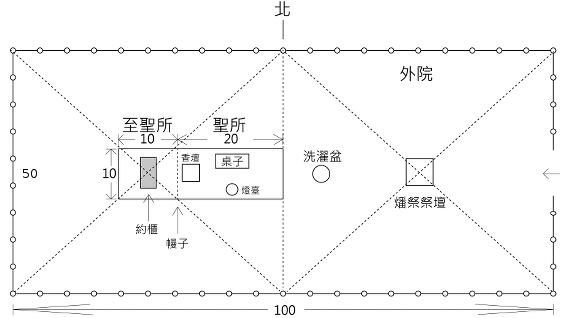
\includegraphics[width=5in]{AMoXiFigs/chuaiji/HuiMu}
%\caption{聖所}
\label{fig:sub1}
\end{figure}
\begin{figure}%{.5\linewidth}
\centering
%
\includegraphics{AMoXiFigs/HuiMuTu.gif}
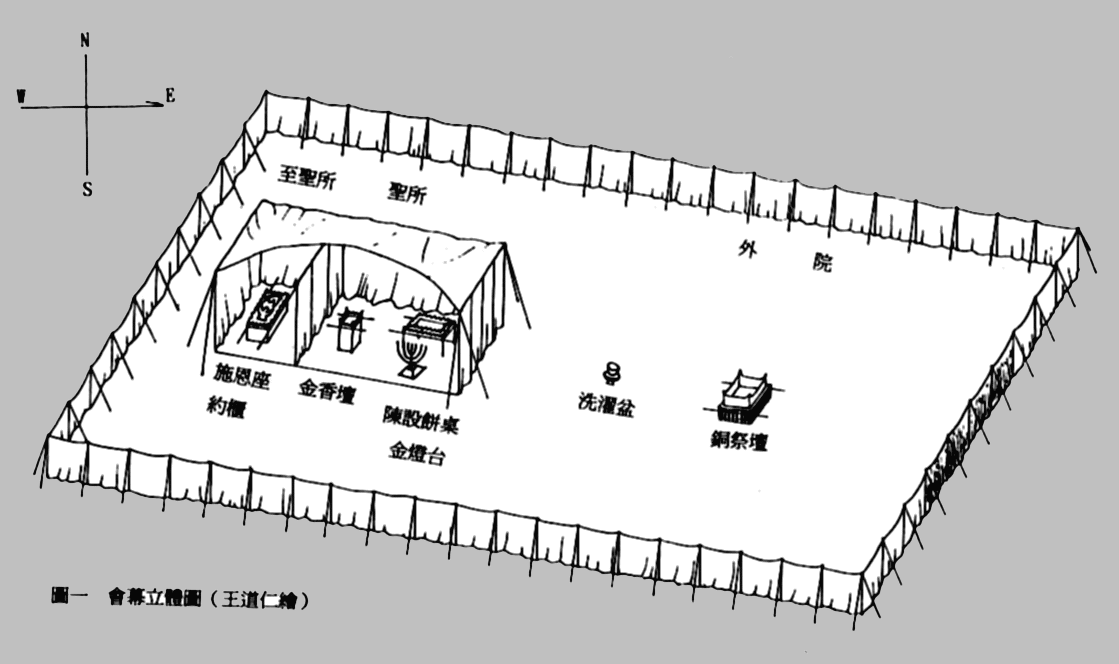
\includegraphics[width=5in]{AMoXiFigs/chuaiji/HuiMuTu}
%\caption{聖所}
\label{fig:sub1}
\end{figure}

\begin{itemize} 
\itemsep-.35em
\item 耶和華曉諭摩西說:你告訴以色列人當為我送禮物來，凡甘心樂意的你們就可以收下歸我。所要收的禮物是
\begin{table}[H]
\centering
\begin{tabular}{|c|c| }
\hline
\hline
材料 & 名稱  \\\hline
金屬 & 金、銀、銅    \\\hline
線類&藍色、紫色、朱紅色線、細麻、山羊毛  \\\hline
皮類&染紅的公羊皮、海狗皮 \\\hline
木類&　皂莢木 　\\\hline
油、香料&點燈的油並做膏油和香的香料　\\\hline
寶石&紅瑪瑙與別樣的寶石，可以鑲嵌在以弗得和胸牌上 \\\hline
\end{tabular}
\caption{奉獻的物}
\end{table}
\item 又當為我造聖所，使我可以住在他們中間。製造帳幕和其中的一切器具，都要照我所指示你的樣式
\end{itemize}

\subsubsection{造約櫃之法則 25:10-22 （37:1-9）}
\begin{itemize} 
\itemsep-.35em
\item 造約櫃之法則
\begin{table}[H]
\centering
\begin{tabular}{|c|l| }
\hline
\hline
部件 & 规格  \\\hline
約櫃 & 皂莢木，長2.5肘 X 寬1.5肘 X 高1.5肘，裡外包上精金、四圍鑲上金牙邊    \\\hline
金環&鑄四個金環安在櫃的四腳上、這邊兩環、那邊兩環。   \\\hline
抬杠&用皂莢木做兩根槓用金包裹。要把槓穿在櫃旁的環內以便抬櫃。這槓要常在櫃的環內，不可抽出來\\\hline
櫃裡&必將我所要賜給你的法版放在櫃裡　\\\hline
施恩座&要用精金做施恩（蔽罪）座，要將施恩座安在櫃的上邊，長2.5肘 X 寬1.5肘　\\\hline
基路伯&要用金子錘出兩個基路伯來，安在施恩座的兩頭。二基路伯要接連一塊。二基路伯要高張翅膀\\
&遮掩施恩座。基路伯要臉對臉，朝著施恩座。要將施恩座安在櫃的上邊  \\\hline
\end{tabular}
\caption{造約櫃之法則}
\end{table}
\item 我要在那裡與你相會，又要從法櫃施恩座上二基路伯中間，和你說我所要吩咐你傳給以色列人的一切事
\end{itemize}

\subsubsection{造陳設餅的桌子及器皿 25:23-30  （37:10-16）}
\begin{table}[H]
\centering
\begin{tabular}{|c|l| }
\hline
\hline
部件 & 规格   \\\hline
桌子 &要用皂莢木做一張桌子，長2肘 X 寬1肘 X 高1肘，包上精金、四圍鑲上金牙邊    \\\hline
橫梁&桌子的四圍各作一掌寬的橫梁、橫梁上鑲著金牙邊。    \\\hline
金環&要做四個金環安在桌子的四角上，就是桌子四腳上的四角。安環子的地方要挨近橫梁可以穿槓抬桌子\\\hline
兩根杠&要用皂莢木做兩根槓，用金包裹，以便抬桌子\\\hline
桌子上&要做桌子上的盤子、調羹，並奠酒的爵和瓶，這都要用精金製作\\\hline
陳設餅&又要在桌子上，在我面前，常擺陳設餅 \\\hline
\end{tabular}
\caption{造陳設餅的桌子及器皿}
\end{table}

\subsubsection{造燈台 25:31-40 （37:17-24）}
\begin{table}[H]
\centering
\begin{tabular}{|c|l| }
\hline
\hline
部件 & 规格  \\\hline
燈臺&要用精金做一個燈臺。燈臺的座和幹與杯、球、花都要接連一塊錘出來  \\\hline
枝子&燈臺兩旁要杈出六個枝子，這旁三個，那旁三個。  \\\hline
燈臺侧&這旁每枝上有三個杯，形狀像杏花，有球，有花；那旁也如此。從燈臺杈出來的六個枝子都是如此。 \\\hline
燈臺上&燈臺上有四個杯，形狀像杏花，有球，有花。燈臺每兩個枝子以下有球與枝子接連一塊，\\
          &燈臺出的六個枝子都是如此。球和枝子要接連一塊，都是一塊精金錘出來的。\\\hline
燈盞&要做燈臺的七個燈盞，祭司要點這燈，使燈光對照\\\hline
其他&燈臺的蠟剪和蠟花盤也是要精金的  \\\hline
材质&做燈臺和這一切的器具要用精金一他連得，要謹慎做這些物件，都要照著在山上指示你的樣式  \\\hline
\end{tabular}
\caption{燈臺和一切的器具用精金一他連得}
\end{table}


\subsubsection{造帳幕的幔子 26:1-6 （36:8-13）}
\begin{itemize} 
\itemsep-.35em
\item 你要用十幅幔子做帳幕。這些幔子要用撚的細麻和藍色、紫色、朱紅色線製造，並用用巧匠的手工繡上基路伯。幔子都要一樣的尺寸。這五幅幔子要幅幅相連，那五幅幔子也要幅幅相連。 
\item 在這相連的幔子末幅邊上要做50藍色的紐扣，在那相連的幔子末幅邊上也要照樣做，都要兩兩相對，又要做五十個金鉤，用鉤使幔子相連，這才成了一個帳幕。
\end{itemize}
\begin{table}[H]
\centering
\begin{tabular}{|c|c|c|c|}
\hline
\hline
 名稱   & 數目& 尺寸     & 材料  \\\hline
帳幕    &10  & 長28肘 X 寬4肘&撚的細麻+線（藍色紫色朱紅色） \\\hline
鈕扣&50X2&           &藍色 \\\hline
金鉤&50 &                  &  精金  \\\hline
\end{tabular}
\caption{造帳幕和幔子}
\end{table}


\subsubsection{造會幕罩篷之法則 26:7-14 （36:14-19）}
\begin{itemize} 
\itemsep-.35em
\item 你要用山羊毛織十一幅幔子，作為帳幕以上的罩篷。每幅幔子要長三十寬四肘，十一幅幔子都要一樣尺寸，要把五幅幔子連成一幅，又把六幅幔子連成一幅，這第六幅幔子要在罩篷的前面摺上去
\item 在這相連的幔子末幅邊上要做五十個紐扣，在那相連的幔子末幅邊上也做五十個紐扣。又要做五十個銅鉤，鉤在紐扣中，使罩篷連成一個。罩篷的幔子所餘那垂下來的半幅幔子，要垂在帳幕的後頭。罩篷的幔子所餘長的，這邊一肘，那邊一肘，要垂在帳幕的兩旁，遮蓋帳幕
\item 又要用染紅的公羊皮做罩篷的蓋，再用海狗皮做一層罩篷上的頂蓋
\begin{table}[H]
\centering
\begin{tabular}{|c|c|c|c| }
\hline
\hline
名稱   & 數目& 尺寸     & 材料  \\\hline
罩棚& 11幅一樣的尺寸幔子     &每幅長30肘 X 寬4肘&山羊毛織\\\hline
鈕扣& 相連的幔子末幅邊上要各做50X2個紐扣     & & \\\hline
罩棚鉤& 50鉤在紐扣中，使罩篷連成一個     & &銅\\\hline
罩棚蓋&2层，罩篷的蓋+做一層罩篷上的頂蓋       & &染紅的公羊皮+海狗皮\\\hline
\end{tabular}
\caption{造會幕罩篷之法則}
\end{table}
\end{itemize}

\subsubsection{造幕板之法則 26:15-30 （36:20-34）}
\begin{itemize} 
\itemsep-.35em
\item 你要用皂莢木做帳幕的豎板。每塊要長十肘，寬一肘半，每塊必有兩榫相對。帳幕一切的板都要這樣做。帳幕的南面要做板二十塊。在這二十塊板底下要做四十個帶卯的銀座，兩卯接這塊板上的兩榫，兩卯接那塊板上的兩榫。帳幕第二面，就是北面，也要做板二十塊，和帶卯的銀座四十個，這板底下有兩卯，那板底下也有兩卯。帳幕的後面，就是西面，要做板六塊。帳幕後面的拐角要做板兩塊。板的下半截要雙的，上半截要整的，直頂到第一個環子，兩塊都要這樣做兩個拐角。必有八塊板和十六個帶卯的銀座，這板底下有兩卯，那板底下也有兩卯
\item 你要用皂莢木做閂，為帳幕這面的板做五閂，為帳幕那面的板做五閂，又為帳幕後面的板做五閂。板腰間的中閂要從這一頭通到那一頭。板要用金子包裹，又要做板上的金環套閂，閂也要用金子包裹。要照著在山上指示你的樣式立起帳幕
\begin{table}[H]
\centering
\begin{tabular}{|c|c|c|c| }
\hline
\hline
名稱   & 數目& 尺寸     & 材料  \\\hline
南面豎板&   20    &長10肘 X 寬1.5肘 &金子包裹皂莢木，塊板底下要做卯座\\\hline
南面卯座&  40    &                           &銀\\\hline
北面豎板&   20    &長10肘 X 寬1.5肘 &金子包裹皂莢木\\\hline
北面卯座&  40    &                           &銀\\\hline
西面豎板&   8    &長10肘 X 寬1.5肘 &金子包裹皂莢木\\\hline
西面卯座&  16    &                          &銀\\\hline
柱子&   4    &                                  &包金的皂莢木，柱子上有金鉤\\\hline
柱子卯座&  4    &  &銀\\\hline
板閂&  15    &  &左右各5，後面5，包金的皂莢木，金環套閂\\\hline
\end{tabular}
\caption{造幕板之法則}
\end{table}
\end{itemize}

\subsubsection{造聖所與至聖所隔幔之法則 26:31-37 （36:35-38）}
\begin{itemize} 
\itemsep-.35em
\item 你要用藍色、紫色、朱紅色線和撚的細麻織幔子，以巧匠的手工繡上基路伯。要把幔子掛在四根包金的皂莢木柱子上，柱子上當有金鉤，柱子安在四個帶卯的銀座上。要使幔子垂在鉤子下，把法櫃抬進幔子內，這幔子要將聖所和至聖所隔開。又要把施恩座安在至聖所內的法櫃上，把桌子安在幔子外帳幕的北面，把燈臺安在帳幕的南面，彼此相對
\item 你要拿藍色、紫色、朱紅色線和撚的細麻，用繡花的手工織帳幕的門簾。要用皂莢木為簾子做五根柱子，用金子包裹，柱子上當有金鉤，又要為柱子用銅鑄造五個帶卯的座
\begin{table}[H]
\centering
\begin{tabular}{|c|c|c|c| }
\hline
\hline
名稱   & 數目& 尺寸     & 材料  \\\hline
帳幕的門簾&       & &藍色紫色朱紅色線、和撚的細麻\\\hline
門簾柱子&   5    & &皂莢木金子包裹柱子上當有金鉤\\\hline
門簾柱子卯座& 5    &  &銅\\\hline
\end{tabular}
\caption{造聖所與至聖所隔幔之法則}
\end{table}
\end{itemize}

\subsubsection{造祭壇 27:1-8 （38:1-7）}
\begin{table}[H]
\centering
\begin{tabular}{|c|l| }
\hline
\hline
名稱 & 规格  \\\hline
壇 &你要用皂莢木做壇。這壇要四方的，長5肘 X 寬5肘 X 高3肘，包上銅，要用板做壇，壇是空的，都照著在山上指示你的樣式做 \\\hline
拐角&要在壇的四拐角上做四個角，與壇接連一塊，用銅把壇包裹  \\\hline
盆&要做盆，收去壇上的灰，用銅作    \\\hline
其它&又做鏟子、盤子、肉叉子、火鼎，壇上一切的器具都用銅做 \\\hline
銅網& 要為壇做一個銅網，安在壇四面的圍腰板以下、使網從下達到壇的半腰。 \\\hline
銅環&在網的四角上做四個銅環\\\hline
杠&又要用皂莢木為壇做槓，用銅包裹，這槓要穿在壇兩旁的環子內，用以抬壇\\\hline
\end{tabular}
\caption{祭壇}
\end{table}

\subsubsection{帳幕的院子 27:9-19 （38:9-20）}
\begin{itemize} 
\itemsep-.35em
\item 你要做帳幕的院子。院子的\underline{南面}要用撚的細麻做帷子，長一百肘。 10 帷子的柱子要二十根，帶卯的銅座二十個，柱子上的鉤子和杆子都要用銀子做。 
\item \underline{北面}也當有帷子，長一百肘，帷子的柱子二十根，帶卯的銅座二十個，柱子上的鉤子和杆子都要用銀子做。
\item 院子的\underline{西面}當有帷子，寬五十肘，帷子的柱子十根，帶卯的座十個
\item 院子的\underline{東面}要寬五十肘。門這邊的帷子要十五肘，帷子的柱子三根，帶卯的座三個。門那邊的帷子也要十五肘，帷子的柱子三根，帶卯的座三個。
\item \underline{院子的門}當有\underline{簾子}，長二十肘，要拿藍色、紫色、朱紅色線和撚的細麻，用繡花的手工織成，柱子四根，帶卯的座四個。\underline{院子四圍}一切的柱子都要用銀杆連絡，柱子上的鉤子要用銀做，帶卯的座要用銅做。院子要長一百肘，寬五十肘，高五肘，帷子要用撚的細麻做，帶卯的座要用銅做。帳幕各樣用處的器具，並帳幕一切的橛子，和院子裡一切的橛子，都要用銅做。
\end{itemize}

\begin{table}[H]
\centering
\begin{tabular}{|c|c|c|c| }
\hline
\hline
 名稱   & 數目& 尺寸     & 材料  \\\hline
南面帷子&       &100肘X 5肘    &撚的細麻\\\hline
南面帷子的柱子&  20    & &柱子上的鉤子和杆子用銀子作\\\hline
南面帷子卯座&  20    &  &銅\\\hline

北面帷子&       &100肘X 5肘  &撚的細麻\\\hline
北面帷子的柱子&  20    & &柱子上的鉤子和杆子用銀子作\\\hline
北面帷子卯座&  20    &  &銅\\\hline

西面帷子&       &50肘X 5肘  &撚的細麻\\\hline
西面帷子的柱子&  10    & &柱子上的鉤子和杆子用銀子作\\\hline
西面帷子卯座&  10    &  &銅\\\hline

門這邊帷子&   2    &15肘X 5肘  &撚的細麻\\\hline
門這邊帷子的柱子&  3X2+4    & &柱子上的鉤子和杆子用銀子作\\\hline
門這邊帷子卯座& 3X2+4 &  &銅\\\hline
門簾&  20    &  &細麻+線（藍色紫色朱紅色）用繡花的手工織成\\\hline
橛子& &  &銅\\\hline
\end{tabular}
\caption{帳幕的院子}
\end{table}


\subsubsection{燃燈的律例 27:20-21 （利未記24:1-4）}
\begin{itemize} 
\itemsep-.35em
\item 你要吩咐以色列人，把那為點燈搗成的清橄欖油拿來給你，使燈常常點著。在會幕中法櫃前的幔外
\item 亞倫和他的兒子，從晚上到早晨，要在耶和華面前經理這燈。這要做以色列人世世代代永遠的定例
\end{itemize} 

\subsubsection{制作祭司服饰的条例 28}
%\subsubsection{祭司服饰图}
\begin{figure*}[t!]
    \centering
    \begin{subfigure}[b]{0.5\textwidth}
        \centering
        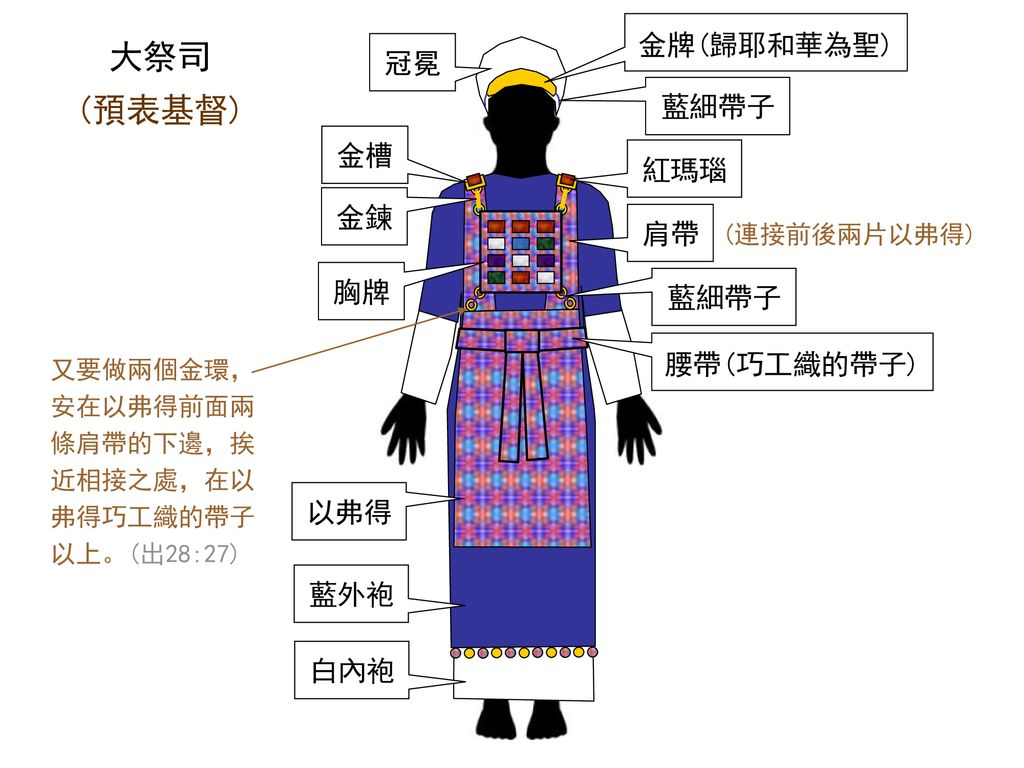
\includegraphics[height=2.5in]{AMoXiFigs/chuaiji/prest2}
       % \caption{}
    \end{subfigure}%
    ~ 
    \begin{subfigure}[b]{0.5\textwidth}
        \centering
        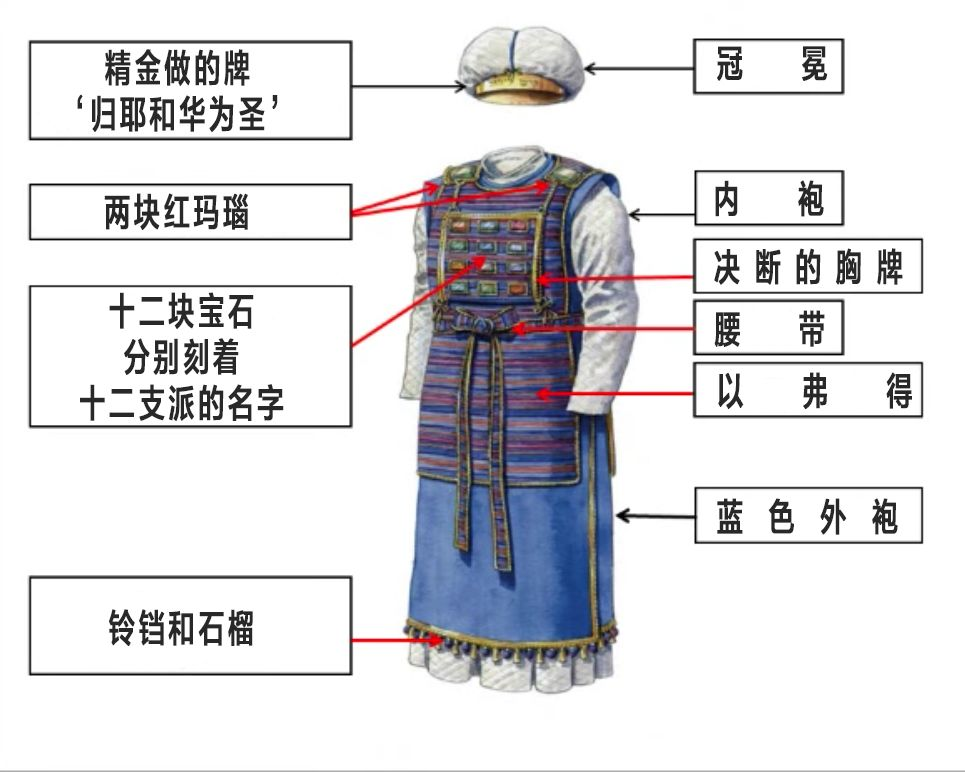
\includegraphics[height=2.5in]{AMoXiFigs/chuaiji/highprest}
      %  \caption{}
    \end{subfigure}
    \caption{祭司服饰图}
\end{figure*}

\subsubsubsection{命亞倫及其后裔為祭司并为其做聖衣 28:1-5}
\begin{itemize} 
\itemsep-.35em
\item 你要從以色列人中，使你的哥哥亞倫和他的兒子拿答、亞比戶、以利亞撒、以他瑪一同就近你，給我供祭司的職分。你要給你哥哥亞倫做聖衣為榮耀，為華美。 
\item 又要吩咐一切心中有智慧的，就是我用智慧的靈所充滿的，給亞倫做衣服，使他分別為聖，可以給我供祭司的職分。所要做的就是胸牌、以弗得、外袍、雜色的內袍、冠冕、腰帶，使你哥哥亞倫和他兒子穿這聖服，可以給我供祭司的職分。要用金線和藍色、紫色、朱紅色線並細麻去做
\end{itemize}
\begin{table}[H]
\centering
\begin{tabular}{|c|c|c| }
\hline
\hline
名稱 &材質　&　章節\\\hline
外袍 & 藍的& 28：31-35 \\\hline
胸牌&（1虎口 X 1虎口）胸牌貼在以弗得巧工織的帶子上&　28：15-30 \\\hline
以弗得&金線和藍色紫色朱紅色線、並撚的細麻&28：6-14　\\\hline
面牌&精金作、在上面刻著、歸耶和華為聖。這牌必在亞倫的額上&28：32-38　\\\hline
內袍&雜色細麻線織&　28：39\\\hline
冠冕&細麻布作&28：39　\\\hline
腰帶&繡花的手工作腰帶&28：39　\\\hline
褲子&細麻布。遮掩下體．褲子當從腰達到大腿&　28：42\\\hline
裹頭巾&亞倫的兒子用&　28：40\\\hline
\end{tabular}
\caption{祭司的服裝}
\end{table}

\subsubsubsection{做以弗得 28:6-14（39:2-7）}
\begin{wrapfigure}{r}{0.3\textwidth}
\vspace{-20pt}
\begin{center}
    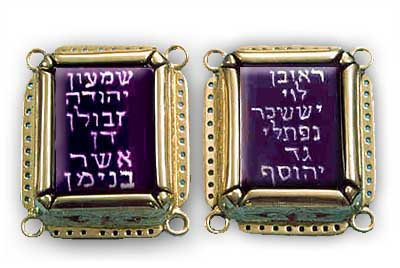
\includegraphics[width=0.3\textwidth]{AMoXiFigs/chuaiji/RedMaNao}
\end{center}
\vspace{-20pt}
  \caption{紅瑪瑙}
 \vspace{-10pt}
\end{wrapfigure}
他們要拿金線和藍色、紫色、朱紅色線並撚的細麻，用巧匠的手工做以弗得。以弗得當有兩條肩帶，接上兩頭，使它相連。其上巧工織的帶子，要和以弗得一樣的做法，用以束上，與以弗得接連一塊，要用金線和藍色、紫色、朱紅色線並撚的細麻做成。
要取兩塊紅瑪瑙，在上面刻以色列兒子的名字，六個名字在這塊寶石上，六個名字在那塊寶石上，都照他們生來的次序。要用刻寶石的手工，彷彿刻圖書，按著以色列兒子的名字刻這兩塊寶石，要鑲在金槽上。要將這兩塊寶石安在以弗得的兩條肩帶上，為以色列人做紀念石。亞倫要在兩肩上擔他們的名字，在耶和華面前作為紀念。
要用金子做二槽，又拿精金，用擰工彷彿擰繩子，做兩條鏈子，把這擰成的鏈子搭在二槽上。


\begin{table}[H]
\centering
\begin{tabular}{|c|c| }
\hline
\hline
材料 & 名稱  \\\hline
以弗得 & 細麻+線（金線，藍色，紫色，朱紅色）   \\\hline
兩條肩帶&細麻+線（金線，藍色，紫色，朱紅色）    \\\hline
兩塊紅瑪瑙&鑲金槽刻以色列兒子的名字 \\\hline
兩條鍊子&　精金、用擰工彷彿擰繩子　\\\hline
\end{tabular}
\caption{以弗得}
\end{table}



\subsubsubsection{做胸牌 28:15-30，39:8-21}
\iffalse
\begin{wraptable}{r}{7.5cm}
\begin{table}[H]
\centering
\begin{tabular}{|c|c|c|c| }
\hline
\hline
第一行 & 紅寶石&紅璧璽&紅玉  \\\hline
第二行&綠寶石&藍寶石&金鋼石  \\\hline
第三行&紫瑪瑙&白瑪瑙&紫晶。 \\\hline
第四行&　水蒼玉&紅瑪瑙&碧玉　\\\hline
\end{tabular}
\caption{胸牌}
\end{table}
\end{wrapfigure}
\fi
你要用巧匠的手工做一個決斷的胸牌。要和以弗得一樣的做法，用金線和藍色、紫色、朱紅色線並撚的細麻做成。這胸牌要四方的，疊為兩層，長一虎口，寬一虎口。要在上面鑲寶石四行：第一行是紅寶石、紅璧璽、紅玉，第二行是綠寶石、藍寶石、金鋼石，第三行是紫瑪瑙、白瑪瑙、紫晶，第四行是水蒼玉、紅瑪瑙、碧玉。這都要鑲在金槽中。
\begin{wrapfigure}{r}{0.3\textwidth}
\vspace{-20pt}
\begin{center}
    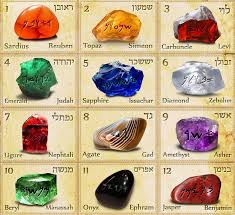
\includegraphics[width=0.3\textwidth]{AMoXiFigs/chuaiji/stones}
\end{center}
\vspace{-10pt}
  \caption{胸牌}
 \vspace{-10pt}
\end{wrapfigure}
這些寶石都要按著以色列十二個兒子的名字，彷彿刻圖書，刻十二個支派的名字。要在胸牌上用精金擰成如繩的鏈子。在胸牌上也要做兩個金環，安在胸牌的兩頭。要把那兩條擰成的金鏈子，穿過胸牌兩頭的環子。又要把鏈子的那兩頭接在兩槽上，安在以弗得前面肩帶上。要做兩個金環，安在胸牌的兩頭，在以弗得裡面的邊上。又要做兩個金環，安在以弗得前面兩條肩帶的下邊，挨近相接之處，在以弗得巧工織的帶子以上。要用藍細帶子把胸牌的環子與以弗得的環子繫住，使胸牌貼在以弗得巧工織的帶子上，不可與以弗得離縫。

亞倫進聖所的時候，要將決斷胸牌，就是刻著以色列兒子名字的，戴在胸前，在耶和華面前常做紀念。又要將烏陵和土明放在決斷的胸牌裡。亞倫進到耶和華面前的時候，要戴在胸前，在耶和華面前常將以色列人的決斷牌戴在胸前


\begin{table}[H]
    \begin{minipage}{.5\linewidth}
      \centering
       \begin{tabular}{|c|c|c|c| }
\hline
\hline
第一行 & 紅寶石&紅璧璽&紅玉  \\\hline
第二行&綠寶石&藍寶石&金鋼石  \\\hline
第三行&紫瑪瑙&白瑪瑙&紫晶。 \\\hline
第四行&　水蒼玉&紅瑪瑙&碧玉　\\\hline
\end{tabular}
   \caption{胸牌}
    \end{minipage}%
    \begin{minipage}{.5\linewidth}
      \centering    
     \begin{tabular}{|c|c| }
\hline
\hline
外袍 & 藍的  \\\hline
領口&口的周圍織出領邊  \\\hline
石榴&藍色+紫色+朱紅色線 \\\hline
金鈴鐺&金　\\\hline
\end{tabular}
%  \caption{以弗得外袍}
    \end{minipage} 
\end{table}


\subsubsubsection{製造以弗得外袍的規定 28:31-35（39:22-26）}
\begin{itemize} 
\itemsep-.35em
\item 你要做以弗得的外袍顏色全是藍的。袍上要為頭留一領口，口的周圍織出領邊來彷彿鎧甲的領口免得破裂
\item 袍子周圍底邊上要用藍色、紫色、朱紅色線做石榴，在袍子周圍的石榴中間要有金鈴鐺。一個金鈴鐺一個石榴，一個金鈴鐺一個石榴，在袍子周圍的底邊上。
\item 亞倫供職的時候要穿這袍子。他進聖所到耶和華面前以及出來的時候，袍上的響聲必被聽見使他不至死亡
\end{itemize}


\subsubsubsection{製造面牌的規定 28:36-38}
\begin{itemize} 
\itemsep-.35em
\item 你要用精金做一面牌，在上面按刻圖書之法刻著：歸耶和華為聖。要用一條藍細帶子將牌繫在冠冕的前面。
\item 這牌必在亞倫的額上，亞倫要擔當干犯聖物條例的罪孽，這聖物是以色列人在一切的聖禮物上所分別為聖的。這牌要常在他的額上，使他們可以在耶和華面前蒙悅納。
\end{itemize}

\subsubsubsection{製造內袍冠冕腰帶裹頭巾褲子 28:39-43（39:27-29）}
\begin{itemize} 
\itemsep-.35em
\item 要用雜色細麻線織內袍，用細麻布做冠冕，又用繡花的手工做腰帶。你要為亞倫的兒子做內袍、腰帶、裹頭巾，為榮耀，為華美。要把這些給你的哥哥亞倫和他的兒子穿戴，又要膏他們，將他們分別為聖，好給我供祭司的職分。 
\item 要給他們做細麻布褲子，遮掩下體，褲子當從腰達到大腿。亞倫和他兒子進入會幕，或就近壇，在聖所供職的時候必穿上，免得擔罪而死。這要為亞倫和他的後裔做永遠的定例
\end{itemize}

\subsubsection{祭司分别为圣的禮仪 29}
\subsubsubsection{祭司承接聖職的穿戴 29:1-9 }
\begin{itemize} 
\itemsep-.35em
\item 你使亞倫和他兒子成聖，給我供祭司的職分，要如此行。
\begin{itemize} 
\itemsep-.35em
\item 献祭：取一隻\underline{公牛犢}，兩隻無殘疾的\underline{公綿羊}，\underline{無酵餅}和\underline{調油的無酵餅}，與\underline{抹油的無酵薄餅}，這都要用細麥麵做成。這餅要裝在一個筐子裡，連筐子帶來，又把公牛和兩隻公綿羊牽來。
\item 要使亞倫和他兒子到會幕門口來用水洗身。 
\begin{itemize} 
\itemsep-.35em
\item 要給亞倫穿上內袍和以弗得的外袍並以弗得，又戴上胸牌，束上以弗得巧工織的帶子。 6 把冠冕戴在他頭上，將聖冠加在冠冕上，就把膏油倒在他頭上膏他。 
\item 要叫他的兒子來，給他們穿上內袍。 
\item 給亞倫和他兒子束上腰帶，包上裹頭巾，
\end{itemize} 
\end{itemize}
\item 他們就憑永遠的定例得了祭司的職任。又要將亞倫和他兒子分別為聖
\end{itemize}


\subsubsubsection{承接聖職的贖罪祭-公牛 29:10-14 （利8:14-17）}
\begin{itemize} 
\itemsep-.35em
\item 你要把公牛牽到會幕前，亞倫和他兒子要按手在公牛的頭上。 
\item 你要在耶和華面前，在會幕門口，宰這公牛。要取些公牛的血，用指頭抹在壇的四角上，把血都倒在壇腳那裡。要把一切蓋臟的脂油與肝上的網子，並兩個腰子和腰子上的脂油，都燒在壇上。只是公牛的皮、肉、糞都要用火燒在營外。這牛是\underline{贖罪祭}
\end{itemize}

\subsubsubsection{承接聖職的燔祭-一隻公綿羊 29:15-18 （利8:18-21）}
\begin{itemize} 
\itemsep-.35em
\item 你要牽一隻公綿羊來，亞倫和他兒子要按手在這羊的頭上。 
\item 要宰這羊，把血灑在壇的周圍。要把羊切成塊子，洗淨五臟和腿，連塊子帶頭，都放在一處。要把全羊燒在壇上，是給耶和華獻的\underline{燔祭}，是獻給耶和華為馨香的\underline{火祭}
\end{itemize}

\subsubsubsection{承接聖職的公綿羊-搖祭及舉祭 29:19-25 （利8:22-29）}
\begin{itemize} 
\itemsep-.35em
\item 你要將那一隻公綿羊牽來，亞倫和他兒子要按手在羊的頭上。你要宰這羊，取點血抹在亞倫的右耳垂上和他兒子的右耳垂上，又抹在他們右手的大拇指上和右腳的大拇指上，並要把血灑在壇的四圍。你要取點膏油和壇上的血，彈在亞倫和他的衣服上，並他兒子和他兒子的衣服上，\underline{他們和他們的衣服就一同成聖} 。 
\item 搖祭放在燔祭上燒=馨香的火祭
\begin{itemize} 
\itemsep-.35em
\item 你要取這羊的脂油和肥尾巴，並蓋臟的脂油與肝上的網子，兩個腰子和腰子上的脂油並右腿，這是承接聖職所獻的羊。再從耶和華面前裝無酵餅的筐子中取一個餅，一個調油的餅和一個薄餅，都放在亞倫的手上和他兒子的手上，作為\underline{搖祭}，在耶和華面前搖一搖。
\item 要從他們手中接過來，\underline{燒在}耶和華面前壇上的\underline{燔祭}上，是獻給耶和華為馨香的\underline{火祭}。
\end{itemize}
\end{itemize}

\subsubsubsection{承接聖職的其他禮儀 29:29-37 （利8:30-35）}
\begin{itemize} 
\itemsep-.35em
\item 亞倫的聖衣要留給他的子孫，可以穿著受膏，又穿著承接聖職。他的子孫接續他當祭司的，每逢進會幕在聖所供職的時候，要穿七天。
\item 你要將承接聖職所獻公羊的肉煮在聖處。亞倫和他兒子要在會幕門口吃這羊的肉和筐內的餅。他們吃那些贖罪之物，好承接聖職，使他們成聖；只是外人不可吃，因為這是聖物。那承接聖職所獻的肉或餅，若有一點留到早晨，就要用火燒了，不可吃這物，因為是聖物。
\item 你要這樣照我一切所吩咐的，向亞倫和他兒子行承接聖職的禮七天。每天要獻公牛一隻為贖罪祭。你潔淨壇的時候，壇就潔淨了，且要用膏抹壇，使壇成聖。要潔淨壇七天，使壇成聖，壇就成為至聖。凡挨著壇的都成為聖
\end{itemize}


\subsubsubsection{祭司每天當獻的祭物 29:38-46 }
\begin{itemize} 
\itemsep-.35em
\item 你每天所要獻在壇上的就是兩隻一歲的羊羔，早晨要獻這一隻，黃昏的時候要獻那一隻。和這一隻羊羔同獻的，要用細麵伊法十分之一與搗成的油一欣四分之一調和，又用酒一欣四分之一作為奠祭。那一隻羊羔要在黃昏的時候獻上，照著早晨的素祭和奠祭的禮辦理，作為獻給耶和華馨香的火祭。
\item 這要在耶和華面前，會幕門口，做你們世世代代常獻的燔祭。我要在那裡與你們相會，和你們說話。我要在那裡與以色列人相會，會幕就要因我的榮耀成為聖。我要使會幕和壇成聖，也要使亞倫和他的兒子成聖，給我供祭司的職分。
\item 我要住在以色列人中間，做他們的神。他們必知道我是耶和華他們的神，是將他們從埃及地領出來的，為要住在他們中間。我是耶和華他們的神
\end{itemize}
\begin{table}[H]
\centering
\begin{tabular}{|c|c|c|c|c|c|c| }
\hline
\hline
天&贖罪祭 & 燔祭&承接聖職獻的祭 &素祭 &搖祭 & 舉祭\\\hline
1&公牛& 公綿羊（1) &公綿羊（1) & 無酵餅 &無酵餅（1) & 承接聖職公綿羊的腿\\\hline
 &&   & & 調油的無酵餅  & 調油的餅 （1) & \\\hline
 & &   & & 抹油的無酵薄餅 & 薄餅（1) &\\\hline
& &   & &   & 承接聖職公綿羊的胸 & \\\hline
2& 公牛&   & &   &   & \\\hline
3&公牛 &   & &   &   & \\\hline
4&公牛 &   & &   &   & \\\hline
5&公牛 &   & &   &   & \\\hline
6&公牛 &   & &   &   & \\\hline
7&公牛 &   & &   &  & \\\hline
\end{tabular}
\caption{承接聖職獻的7天祭}
\end{table}


\subsubsection{其它会幕物品制作服事條例 30-31}
\subsubsubsection{造香壇的條例 30:1-6，37:25-28}
\begin{itemize} 
\itemsep-.35em
\item 你要用皂莢木做一座燒香的壇。這壇要四方的，長一肘，寬一肘，高二肘。壇的四角要與壇接連一塊。要用精金把壇的上面與壇的四圍並壇的四角包裹
\item 又要在壇的四圍鑲上金牙邊。要做兩個金環安在牙子邊以下，在壇的兩旁兩根橫撐上，作為穿槓的用處，以便抬壇。要用皂莢木做槓，用金包裹。
\item 要把壇放在法櫃前的幔子外，對著法櫃上的施恩座，就是我要與你相會的地方。 
\end{itemize}

\subsubsubsection{亞倫在壇上的服事條例 30:7-10}
\vspace*{-5mm}
 \begin{itemize} 
\itemsep-.35em
\item 亞倫在壇上要燒馨香料做的香，每早晨他收拾燈的時候，要燒這香。黃昏點燈的時候，他要在耶和華面前燒這香，作為世世代代常燒的香。在這壇上不可奉上異樣的香，不可獻燔祭、素祭，也不可澆上奠祭。
\item 亞倫一年一次要在壇的角上行贖罪之禮。他一年一次要用贖罪祭牲的血在壇上行贖罪之禮，作為世世代代的定例。這壇在耶和華面前為至聖。
\end{itemize}

\subsubsubsection{每人當獻贖命之價 30:11-16 （37:25-28）}
\begin{itemize} 
\itemsep-.35em
\item 耶和華曉諭摩西說：「你要按以色列人被數的計算總數，你數的時候，他們各人要為自己的生命把贖價奉給耶和華，免得數的時候在他們中間有災殃。凡過去歸那些被數之人的，每人要按聖所的平，拿銀子半舍客勒，這半舍客勒是奉給耶和華的禮物，一舍客勒是二十季拉。凡過去歸那些被數的人，從二十歲以外的，要將這禮物奉給耶和華。
\item 他們為贖生命將禮物奉給耶和華，富足的不可多出，貧窮的也不可少出，各人要出半舍客勒。你要從以色列人收這贖罪銀，作為會幕的使用，可以在耶和華面前為以色列人做紀念，贖生命。
\end{itemize}

\subsubsubsection{造銅盆的規定 30:17-21 （38:8）}
\begin{itemize} 
\itemsep-.35em
\item 耶和華曉諭摩西說：你要用銅做洗濯盆和盆座，以便洗濯。要將盆放在會幕和壇的中間，在盆裡盛水。
\item 亞倫和他的兒子要在這盆裡洗手洗腳。他們進會幕，或是就近壇前供職給耶和華\underline{獻火祭}的時候，\underline{必用水洗濯}，免得死亡。他們洗手洗腳，就免得死亡。這要做亞倫和他後裔世世代代永遠的定例。
\end{itemize}


\subsubsubsection{製作聖膏油的規定 30:22-33}
\begin{wraptable}{r}{4.2cm}
\vspace*{-\baselineskip}
\begin{tabular}{ll }
\hline
\hline
聖膏油製作& 份量 \\\hline
沒藥 & 500舍客勒 \\\hline
香肉桂&250舍客勒  \\\hline
菖蒲&250舍客勒   \\\hline
桂皮&500舍客勒   \\\hline
橄欖油&1欣 \\\hline
\end{tabular}
\caption{聖膏油的規定}
\end{wraptable}
耶和華曉諭摩西說： 「你要取上品的香料，就是流質的沒藥五百舍客勒，香肉桂一半，就是二百五十舍客勒，菖蒲二百五十舍客勒，桂皮五百舍客勒，都按著聖所的平，又取橄欖油一欣，按做香之法調和做成聖膏油。\\
要用這膏油抹會幕和法櫃，桌子與桌子的一切器具，燈臺和燈臺的器具並香壇，燔祭壇和壇的一切器具，洗濯盆和盆座。要使這些物成為聖，好成為至聖，凡挨著的都成為聖。要膏亞倫和他的兒子，使他們成為聖，可以給我供祭司的職分。\\
你要對以色列人說：『這油，我要世世代代以為聖膏油。不可倒在別人的身上，也不可按這調和之法做與此相似的。這膏油是聖的，你們也要以為聖。凡調和與此相似的，或將這膏膏在別人身上的，這人要從民中剪除。』



\iffalse
\begin{table}[H]
    \begin{subtable}{.5\linewidth}
 \centering  
\begin{tabular}{ll }
\hline
\hline
聖膏油製作& 份量 \\\hline
沒藥 & 500舍客勒 \\\hline
香肉桂&250舍客勒  \\\hline
菖蒲&250舍客勒   \\\hline
桂皮&500舍客勒   \\\hline
橄欖油&1欣 \\\hline
\end{tabular}
\caption{聖膏油和聖香的規定}
    \end{subtable}%
    \begin{subtable}{.5\linewidth}
      \centering    
    \begin{tabular}{ll}
\hline
\hline
聖香製作 &份量\\\hline
 拿他弗 & 1份  \\\hline
  施喜列 &1份 \\\hline
 喜利比拿 &1份  \\\hline
 淨乳香 &1份 \\\hline
 鹽 &\\\hline
\end{tabular}
   \caption{聖香製作}
    \end{subtable} 
\end{table}
\fi

\subsubsubsection{製作聖香的規定 30:34-38}
\begin{wraptable}{r}{5cm}
%\vspace*{-\baselineskip}
\vspace*{-10mm}
   \begin{tabular}{ll}
\hline
\hline
聖香製作 &份量\\\hline
 拿他弗 & 1份  \\\hline
  施喜列 &1份 \\\hline
 喜利比拿 &1份  \\\hline
 淨乳香 &1份 \\\hline
 鹽 &\\\hline
\end{tabular}
\caption{聖香製作}
\end{wraptable}
耶和華吩咐摩西說：「你要取馨香的香料，就是拿他弗、施喜列、喜利比拿，這馨香的香料和淨乳香各樣要一般大的分量。你要用這些加上鹽，按做香之法做成清淨聖潔的香。這香要取點搗得極細，放在會幕內法櫃前，我要在那裡與你相會。\\
你們要以這香為至聖。你們不可按這調和之法為自己做香，要以這香為聖，歸耶和華。凡做香和這香一樣，為要聞香味的，這人要從民中剪除。


\subsubsubsection{神提名比撒列,亞何利亞伯造會幕 31:1-11 （35:30-35）}
%\begin{wraptable}{r}{7.5cm}
\begin{table}[H]
\vspace*{-\baselineskip}
%\vspace*{1.0cm}
\center
\begin{tabular}{ c c c c }
\toprule
支派 & 爺爺名字 & 父親名字& 技工 \\\hline
猶大&戶珥  &  烏利 & 比撒列\\\hline
但&  & 亞希撒抹& 亞何利亞伯 \\\hline
\end{tabular}
\caption{技工比撒列,亞何利亞伯}
\end{table} 
%\end{wraptable}
%\vspace*{-\baselineskip}
耶和華曉諭摩西說：「看哪，猶大支派中，戶珥的孫子、烏利的兒子比撒列，我已經提他的名召他。我也以我的靈充滿了他，使他有智慧，有聰明，有知識，能做各樣的工， 能想出巧工，用金、銀、銅製造各物，又能刻寶石，可以鑲嵌，能雕刻木頭，能做各樣的工。\\
我分派但支派中亞希撒抹的兒子亞何利亞伯與他同工。\underline{\textcolor{blue}{凡}心裡有智慧的，我\textcolor{blue}{更}使他們有智慧，\textcolor{blue}{能}做我一切所吩咐的}，就是會幕和法櫃，並其上的施恩座，與會幕中一切的器具，桌子和桌子的器具，精金的燈臺和燈臺的一切器具並香壇， 燔祭壇和壇的一切器具，並洗濯盆與盆座，精工做的禮服，和祭司亞倫並他兒子用以供祭司職分的聖衣，膏油和為聖所用馨香的香料。他們都要照我一切所吩咐的去做。」
%\end{itemize}


\subsubsubsection{當守安息日為證 31:12-18}
\begin{itemize}
\itemsep-.35em
\item 耶和華曉諭摩西說：「你要吩咐以色列人說：『你們務要守我的安息日，因為這是你我之間世世代代的證據，使你們知道我\underline{耶和華是叫你們成為聖的。所以你們要守安息日，以為聖日}。凡干犯這日的，必要把他治死；凡在這日做工的，必從民中剪除。六日要做工，但第七日是安息聖日，是向耶和華守為聖的。凡在安息日做工的，必要把他治死。故此，以色列人要世世代代守安息日為永遠的約。這是我和以色列人永遠的證據，因為六日之內\underline{耶和華造天地，第七日便安息舒暢}。』」
\item 耶和華在西奈山和摩西說完了話，就把兩塊法版交給他，是神用指頭寫的石版。
\end{itemize}

\subsection{摩西四次上山為百姓拜金牛犢代求 32-34}
\subsubsection{亞倫造犢 32:1-6}
\begin{itemize}
\itemsep-.35em
\item 百姓見摩西遲延不下山，就大家聚集到亞倫那裡，對他說：「起來，為我們做神像，可以在我們前面引路，因為領我們出埃及地的那個摩西，我們不知道他遭了什麼事。」 
\item 亞倫對他們說：「你們去摘下你們妻子、兒女耳上的金環，拿來給我。」
\begin{itemize}
\itemsep-.35em
\item 百姓就都摘下他們耳上的金環，拿來給亞倫。 
 \item 亞倫從他們手裡接過來，鑄了一隻牛犢，用雕刻的器具做成。他們就說：「以色列啊，這是領你出埃及地的神！」亞倫看見，就在牛犢面前築壇，且宣告說：「明日要向耶和華守節。」 
\item 次日清早，百姓起來獻燔祭和平安祭，就坐下吃喝，起來玩耍。
\end{itemize}
\end{itemize}

\subsubsection{摩西第一次為百姓代求 32:7-14}
\begin{table}[H]
\begin{threeparttable}
\begin{tabular}{@{}p{0.4\textwidth}*{4}{L{\dimexpr0.7\linewidth-10\tabcolsep\relax}}@{}}
\toprule
神 &  摩西 \\\hline
耶和華吩咐摩西說：「下去吧，因為你的百姓，就是你從埃及地領出來的，已經敗壞了。他們快快偏離了我所吩咐的道，為自己鑄了一隻牛犢，向它下拜獻祭，說：『以色列啊，這就是領你出埃及地的神！』」&\tabularnewline\hline
耶和華對摩西說：「我看這百姓真是硬著頸項的百姓。你且由著我，我要向他們發烈怒，將他們滅絕，使你的後裔成為大國。」&摩西便懇求耶和華他的神說：「耶和華啊，你為什麼向你的百姓發烈怒呢？這百姓是你用大力和大能的手從埃及地領出來的。為什麼使埃及人議論說『他領他們出去，是要降禍於他們，把他們殺在山中，將他們從地上除滅』？求你轉意，不發你的烈怒；後悔，不降禍與你的百姓。求你記念你的僕人亞伯拉罕、以撒、以色列，你曾指著自己起誓說：『我必使你們的後裔像天上的星那樣多，並且我所應許的這全地，必給你們的後裔，他們要永遠承受為業。』」\tabularnewline\hline
於是耶和華後悔，不把所說的禍降於他的百姓&\tabularnewline
\bottomrule
\end{tabular}
%\caption{摩西第一次為百姓代求}
\end{threeparttable}
\end{table} 


\subsubsection{摩西怒摔法版 32:15-29}
\begin{itemize}
\itemsep-.35em
\item 摩西轉身下山手裡拿著兩塊法版。這版是兩面寫的這面那面都有字，是神的工作，字是神寫的刻在版上。約書亞一聽見百姓呼喊的聲音，就對摩西說：「在營裡有爭戰的聲音。」摩西說：「這不是人打勝仗的聲音，也不是人打敗仗的聲音，我所聽見的乃是人歌唱的聲音。」
\item 摩西挨近營前，就看見牛犢，又看見人跳舞，便發烈怒，把兩塊版扔在山下摔碎了，又將他們所鑄的牛犢用火焚燒，磨得粉碎，撒在水面上，叫以色列人喝。摩西對亞倫說：「這百姓向你做了什麼？你竟使他們陷在大罪裡！」亞倫說：「求我主不要發烈怒。這百姓專於作惡，是你知道的。他們對我說：『你為我們做神像，可以在我們前面引路，因為領我們出埃及地的那個摩西，我們不知道他遭了什麼事。』我對他們說：『凡有金環的，可以摘下來。』他們就給了我，我把金環扔在火中，這牛犢便出來了。」
\item 三千百姓被利未的子孫殺死
\begin{table}[H]
\begin{threeparttable}
\begin{tabular}{@{}p{0.6\textwidth}*{4}{L{\dimexpr0.5\linewidth-10\tabcolsep\relax}}@{}}
\toprule
摩西 & 利未的子孫 \\\hline
摩西見百姓放肆（亞倫縱容他們，使他們在仇敵中間被譏刺），就站在營門中，說：「凡屬耶和華的，都要到我這裡來！」&於是利未的子孫都到他那裡聚集。\tabularnewline\hline
他對他們說：「耶和華以色列的神這樣說：『你們各人把刀跨在腰間，在營中往來，從這門到那門，各人殺他的弟兄與同伴並鄰舍。』」 &利未的子孫照摩西的話行了。那一天百姓中被殺的約有三千\tabularnewline\hline
摩西說：「今天你們要自潔，歸耶和華為聖，各人攻擊他的兒子和弟兄，使耶和華賜福於你們。」 &\tabularnewline
\bottomrule
\end{tabular}
\caption{三千百姓被利未的子孫殺死}
\end{threeparttable}
\end{table} 
\end{itemize}

\subsubsection{摩西第二次為百姓代求 32:30-33:3}
\begin{table}[H]
\begin{threeparttable}
\begin{tabular}{@{}p{0.4\textwidth}*{4}{L{\dimexpr0.6\linewidth-10\tabcolsep\relax}}@{}}
\toprule
摩西 &  神 \\\hline
到了第二天，摩西對百姓說:你們犯了大罪，我如今要上耶和華那裡去，或者可以為你們贖罪&\tabularnewline\hline
摩西回到耶和華那裡，說：「唉！這百姓犯了大罪，為自己做了金像。倘或你肯赦免他們的罪——不然，求你從你所寫的冊上塗抹我的名。」&耶和華對摩西說：「誰得罪我，我就從我的冊上塗抹誰的名。現在你去領這百姓，往我所告訴你的地方去，我的使者必在你前面引路，只是到我追討的日子，我必追討他們的罪。」\tabularnewline\hline
&耶和華殺百姓的緣故是因他們同亞倫做了牛犢。\tabularnewline\hline
&耶和華吩咐摩西說：「我曾起誓應許亞伯拉罕、以撒、雅各說：『要將迦南地賜給你的後裔。』現在你和你從埃及地所領出來的百姓，要從這裡往那地去。我要差遣使者在你前面，攆出迦南人、亞摩利人、赫人、比利洗人、希未人、耶布斯人領你到那流奶與蜜之地。我自己不同你們上去，因為你們是硬著頸項的百姓，恐怕我在路上把你們滅絕。」\tabularnewline
\bottomrule
\end{tabular}
%\caption{摩西第二次為百姓代求}
\end{threeparttable}
\end{table} 

\subsubsection{百姓除淨身上佩戴裝飾 33:4-6}
\begin{itemize}
\itemsep-.35em
\item 百姓聽見這凶信就悲哀，也沒有人佩戴裝飾。 
\item 耶和華對摩西說：「你告訴以色列人說：『耶和華說：你們是硬著頸項的百姓，我若一霎時臨到你們中間，必滅絕你們。現在你們要把身上的裝飾摘下來，使我可以知道怎樣待你們。』」 
\item 以色列人從住何烈山以後，就把身上的裝飾摘得乾淨
\end{itemize}

\subsubsection{摩西與神會面的會幕——支搭在的營外帳篷 33:7-11}
\begin{itemize}
\itemsep-.35em
\item 摩西素常將帳篷支搭在營外，離營卻遠，他稱這帳篷為會幕。凡求問耶和華的，就到營外的會幕那裡去。 
\begin{itemize}
\itemsep-.35em
\item 當摩西出營到會幕去的時候，百姓就都起來，各人站在自己帳篷的門口，望著摩西，直等到他進了會幕。
 \item 摩西進會幕的時候，雲柱降下來，立在會幕的門前，耶和華便與摩西說話。
\item 眾百姓看見雲柱立在會幕門前，就都起來，各人在自己帳篷的門口下拜。
\item 耶和華與摩西面對面說話，好像人與朋友說話一般。
\end{itemize}
\item 摩西轉到營裡去，唯有他的幫手，一個少年人嫩的兒子約書亞，不離開會幕。
\end{itemize}


\subsubsection{摩西求耶和華同往,并蒙恩见神的荣耀 33:12-23}
\begin{table}[H]
\begin{threeparttable}
\begin{tabular}{@{}p{0.4\textwidth}*{4}{L{\dimexpr0.7\linewidth-10\tabcolsep\relax}}@{}}
\toprule
摩西的祈祷 &  神的应许 \\\hline
摩西對耶和華說：「你吩咐我說：『將這百姓領上去』，卻沒有叫我知道你要打發誰與我同去，只說：『我按你的名認識你，你在我眼前也蒙了恩。』 我如今若在你眼前蒙恩，求你將你的道指示我，使我可以認識你，好在你眼前蒙恩。求你想到這民是你的民。」&耶和華說：「我必親自和你同去，使你得安息。」\tabularnewline\hline
摩西說：「你若不親自和我同去，就不要把我們從這裡領上去。人在何事上得以知道我和你的百姓在你眼前蒙恩呢？豈不是因你與我們同去，使我和你的百姓與地上的萬民有分別嗎？」&耶和華對摩西說：「你這所求的我也要行，因為你在我眼前蒙了恩，並且我按你的名認識你。」 \tabularnewline\hline
摩西說：「求你顯出你的榮耀給我看。」&耶和華說：「我要顯我一切的恩慈，在你面前經過，宣告我的名。我要恩待誰就恩待誰，要憐憫誰就憐憫誰。」 \tabularnewline\hline
&又說：「你不能看見我的面，因為人見我的面不能存活。」 \tabularnewline\hline
&耶和華說：「看哪，在我這裡有地方，你要站在磐石上。我的榮耀經過的時候，我必將你放在磐石穴中，用我的手遮掩你，等我過去。然後我要將我的手收回，你就得見我的背，卻不得見我的面。」 \tabularnewline
\bottomrule
\end{tabular}
\caption{摩西求耶和華同往,并蒙恩见神的荣耀}
\end{threeparttable}
\end{table} 

\subsubsection{摩西復上西奈山，新鑿兩塊石版 34:1-4 （申10:1-5）}
耶和華吩咐摩西說：「你要鑿出兩塊石版，和先前你摔碎的那版一樣，其上的字我要寫在這版上。明日早晨，你要預備好了，上西奈山，在山頂上站在我面前。誰也不可和你一同上去，遍山都不可有人，在山根也不可叫羊群牛群吃草。」 \\
摩西就鑿出兩塊石版，和先前的一樣。清晨起來，照耶和華所吩咐的上西奈山去，手裡拿著兩塊石版。

\subsubsection{耶和華宣告自己的名 34:5-9}
耶和華在雲中降臨，和摩西一同站在那裡，宣告耶和華的名。耶和華在他面前宣告說：「耶和華，耶和華，是有憐憫有恩典的神，不輕易發怒，並有豐盛的慈愛和誠實。為千萬人存留慈愛，赦免罪孽、過犯和罪惡；萬不以有罪的為無罪，必追討他的罪，自父及子，直到三四代。」 \\
摩西急忙伏地下拜，說：「主啊，我若在你眼前蒙恩，求你在我們中間同行，因為這是硬著頸項的百姓。又求你赦免我們的罪孽和罪惡，以我們為你的產業。」

\subsubsection{耶和華和立約，并禁止百姓拜別神 34:10-17}
耶和華說：「我要立約，要在百姓面前行奇妙的事，是在遍地萬國中所未曾行的。在你四圍的外邦人就要看見耶和華的作為，因我向你所行的是可畏懼的事。我今天所吩咐你的，你要謹守。我要從你面前攆出亞摩利人、迦南人、赫人、比利洗人、希未人、耶布斯人。\\
你要謹慎，\underline{不可}與你所去那地的居民立約，恐怕成為你們中間的網羅；卻要拆毀他們的祭壇，打碎他們的柱像，砍下他們的木偶。\underline{不可}敬拜別神，因為耶和華是忌邪的神，名為忌邪者。只怕你與那地的居民立約，百姓隨從他們的神，就行邪淫，祭祀他們的神，有人叫你，你便吃他的祭物；又為你的兒子娶他們的女兒為妻，他們的女兒隨從她們的神，就行邪淫，使你的兒子也隨從她們的神行邪淫。\underline{不可}為自己鑄造神像。

\subsubsection{守除酵節,安息日,七七節,收藏節 34:16-26}
你要守\underline{除酵節}，照我所吩咐你的，在亞筆月內所定的日期吃無酵餅七天，因為你是這亞筆月內出了埃及。凡\underline{頭生}的都是我的，一切牲畜頭生的，無論是牛是羊，公的都是我的。頭生的驢要用羊羔代贖，若不代贖就要打折牠的頸項。凡頭生的兒子都要贖出來。誰也不可空手朝見我。\\
你六日要做工，第七日要安息；雖在耕種收割的時候，也要安息。在收割初熟麥子的時候要守\underline{七七節}，又在年底要守\underline{收藏節}。你們一切男丁要一年三次朝見主耶和華以色列的神。我要從你面前趕出外邦人，擴張你的境界。你一年三次上去朝見耶和華你神的時候，必沒有人貪慕你的地土。\\
你不可將我祭物的血和有酵的餅一同獻上，逾越節的祭物也不可留到早晨。地裡首先初熟之物要送到耶和華你神的殿。不可用山羊羔母的奶煮山羊羔。\\

\subsubsection{摩西四十晝夜不吃飯不喝水 34:27-28}
耶和華吩咐摩西說：「你要將這些話寫上，因為我是按這話與你和以色列人立約。」摩西在耶和華那裡四十晝夜，也不吃飯，也不喝水。耶和華將這約的話，就是十條誡，寫在兩塊版上。

\subsubsection{摩西面容發光 34:16-26}
摩西手裡拿著兩塊法版下西奈山的時候，不知道自己的面皮因耶和華和他說話就發了光。亞倫和以色列眾人看見摩西的面皮發光，就怕挨近他。摩西叫他們來，於是亞倫和會眾的官長都到他那裡去，摩西就與他們說話。隨後以色列眾人都近前來，他就把耶和華在西奈山與他所說的一切話都吩咐他們。摩西與他們說完了話，就用帕子蒙上臉。但摩西進到耶和華面前與他說話就揭去帕子，及至出來的時候，便將耶和華所吩咐的告訴以色列人。以色列人看見摩西的面皮發光。摩西又用帕子蒙上臉，等到他進去與耶和華說話，就揭去帕子

\subsection{摩西传神的話，造會幕和祭司服 35-40}
\subsubsection{守安息日之例 35:1-2}
摩西招聚以色列全會眾，對他們說：「這是耶和華所吩咐的話，叫你們照著行。六日要做工，第七日乃為聖日，\underline{當向耶和華守為安息聖日}。凡這日之內做工的，必把他治死。當安息日，不可在你們一切的住處生火。」

\subsubsection{呼召會眾獻禮物 35:4-9 （25:1-7）}
\begin{wraptable}{r}{10.5cm}
%\begin{table}[!hbp]
%\centering
%\vspace*{-\baselineskip}
\vspace*{-1cm}
\begin{tabular}{|c|c| }
\hline
\hline
材料 & 名稱  \\\hline
金屬 & 金、銀、銅    \\\hline
線類&藍色、紫色、朱紅色線、細麻、山羊毛  \\\hline
皮類&染紅的公羊皮、海狗皮 \\\hline
木類&　皂莢木 　\\\hline
油、香料&點燈的油並做膏油和香的香料　\\\hline
寶石&紅瑪瑙與別樣的寶石，可以鑲嵌在以弗得和胸牌上 \\\hline
\end{tabular}
\caption{呼召會眾奉獻的物}
%\end{table}
\end{wraptable} 
摩西對以色列全會眾說：「耶和華所吩咐的是這樣：你們中間要拿禮物獻給耶和華，凡樂意獻的，可以拿耶和華的禮物來，就是金，銀，銅，藍色、紫色、朱紅色線，細麻，山羊毛，染紅的公羊皮，海狗皮，皂莢木，點燈的油，並做膏油和香的香料，紅瑪瑙與別樣的寶石，可以鑲嵌在以弗得和胸牌上。

\subsubsection{呼召有智慧的来做神的工及工作内容 35:10-19 (39:32-41)}
你們中間凡心裡有智慧的，都要來做耶和華一切所吩咐的，就是帳幕和帳幕的罩篷，並帳幕的蓋、鉤子、板、閂、柱子、帶卯的座，櫃和櫃的槓，施恩座和遮掩櫃的幔子，桌子和桌子的槓與桌子的一切器具，並陳設餅，燈臺和燈臺的器具，燈盞並點燈的油，香壇和壇的槓，膏油和馨香的香料，並帳幕門口的簾子，燔祭壇和壇的銅網，壇的槓並壇的一切器具，洗濯盆和盆座，院子的帷子和帷子的柱子，帶卯的座和院子的門簾，帳幕的橛子並院子的橛子和這兩處的繩子，精工做的禮服和祭司亞倫並他兒子在聖所用以供祭司職分的聖衣。

\subsubsection{會眾回应獻禮物的呼召 35:20-29}
以色列全會眾從摩西面前退去。凡心裡受感和甘心樂意的，都拿耶和華的禮物來，用以做會幕和其中一切的使用，又用以做聖衣。凡心裡樂意獻禮物的，連男帶女，各將金器，就是胸前針、耳環 (鼻環)、打印的戒指和手釧，帶來獻給耶和華。凡有藍色、紫色、朱紅色線，細麻，山羊毛，染紅的公羊皮，海狗皮的，都拿了來。凡獻銀子和銅給耶和華為禮物的，都拿了來。凡有皂莢木可做什麼使用的，也拿了來。凡心中有智慧的婦女，親手紡線，把所紡的藍色、紫色、朱紅色線和細麻都拿了來。凡有智慧心裡受感的婦女，就紡山羊毛。眾官長把紅瑪瑙和別樣的寶石，可以鑲嵌在以弗得與胸牌上的，都拿了來，又拿香料做香，拿油點燈，做膏油。以色列人，無論男女，凡甘心樂意獻禮物給耶和華的，都將禮物拿來，做耶和華藉摩西所吩咐的一切工。

\subsubsection{呼召做会幕的技工 35:30-36:2 (31:2-6)}
\begin{wraptable}{r}{12.5cm}
%\begin{table}[H]
\vspace*{-\baselineskip}
%\vspace*{3.0cm}
\center
\begin{tabular}{ c c c c l }
\toprule
支派 &爺爺 &父親名字&技工 &擅长\\\hline
猶大&戶珥  &烏利 &比撒列  &能做金銀銅器，刻嵌寶石，雕刻木頭\\\hline
但&  &亞希撒抹&亞何利亞伯 &藍紫朱紅線和細麻繡花、機匠的工\\\hline
\end{tabular}
\caption{技工比撒列,亞何利亞伯}
%\end{table} 
\end{wraptable}
摩西對以色列人說：「\textcolor{blue}{猶大}支派中，戶珥的孫子、烏利的兒子\textcolor{blue}{比撒列}，耶和華已經提他的名召他，又以神的靈充滿了他，使他有智慧、聰明、知識，能做各樣的工，能想出巧工，用金、銀、銅製造各物，又能刻寶石，可以鑲嵌，能雕刻木頭，能做各樣的巧工。 

耶和華又使他和\textcolor{blue}{但}支派中亞希撒抹的兒子\textcolor{blue}{亞何利亞伯}心裡靈明，能教導人。耶和華使他們的心滿有智慧，能做各樣的工，無論是雕刻的工，巧匠的工，用藍色、紫色、朱紅色線和細麻繡花的工並機匠的工，他們都能做，也能想出奇巧的工。
比撒列和亞何利亞伯，並一切心裡有智慧的，就是蒙耶和華賜智慧、聰明，叫他知道做聖所各樣使用之工的，都要照耶和華所吩咐的做工。」凡耶和華賜他心裡有智慧，而且受感前來做這工的，摩西把他們和比撒列並亞何利亞伯一同召來。

\subsubsection{做会幕的材料獻的有餘 36:3-7}
這些人就從摩西收了以色列人為做聖所並聖所使用之工所拿來的禮物。百姓每早晨還把甘心獻的禮物拿來。凡做聖所一切工的智慧人，各都離開他所做的工，來對摩西說：「百姓為耶和華吩咐使用之工所拿來的，富富有餘。」摩西傳命，他們就在全營中宣告說：「無論男女，不必再為聖所拿什麼禮物來。」這樣才攔住百姓不再拿禮物來。因為他們所有的材料夠做一切當做的物，而且有餘。

%\subsection{造會幕和祭司服饰 36:8-39:31}
\subsubsection{造會幕的工作 36:8-13}
他們中間凡心裡有智慧做工的，用十幅幔子做帳幕。這幔子是比撒列用撚的細麻和藍色、紫色、朱紅色線製造的，並用巧匠的手工繡上基路伯。每幅幔子長二十八肘，寬四肘，都是一樣的尺寸。他使這五幅幔子幅幅相連，又使那五幅幔子幅幅相連。在這相連的幔子末幅邊上做藍色的紐扣，在那相連的幔子末幅邊上也照樣做。在這相連的幔子上做五十個紐扣，在那相連的幔子上也做五十個紐扣，都是兩兩相對。又做五十個金鉤，使幔子相連。這才成了一個帳幕。
\begin{figure}[ht]
\centering
\begin{subfigure}{.5\textwidth}
  \centering
  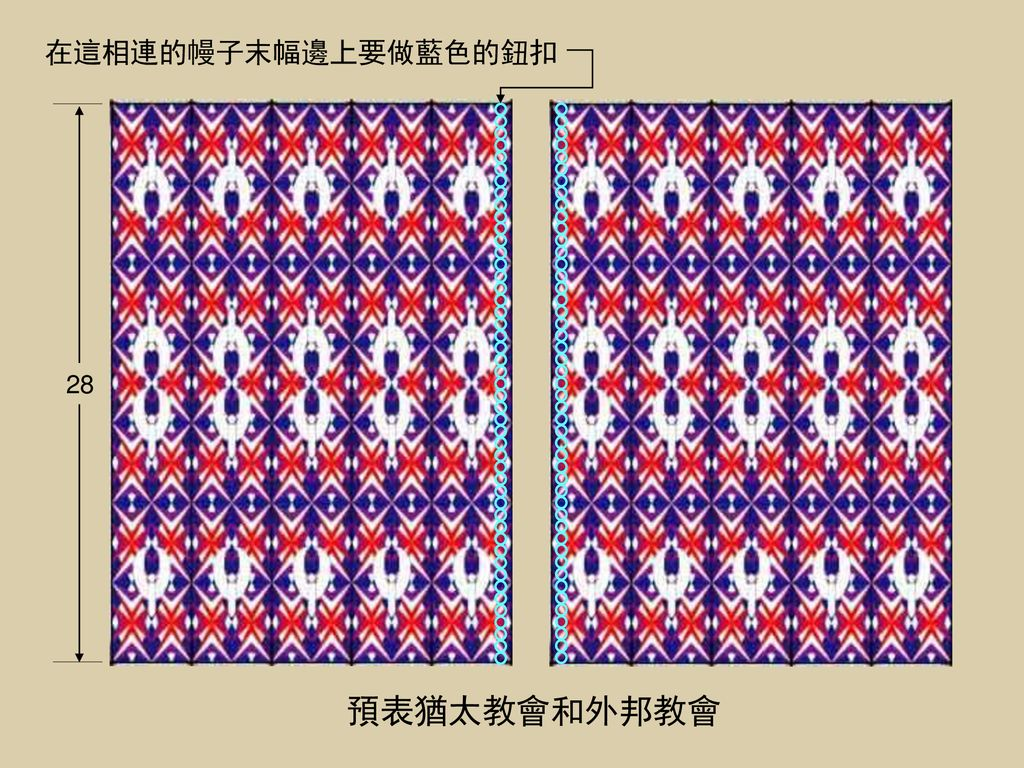
\includegraphics[width=.8\linewidth]{AMoXiFigs/chuaiji/zhangmu12}
 % \caption{A subfigure}
  \label{fig:sub1}
\end{subfigure}%
\begin{subfigure}{.5\textwidth}
  \centering
  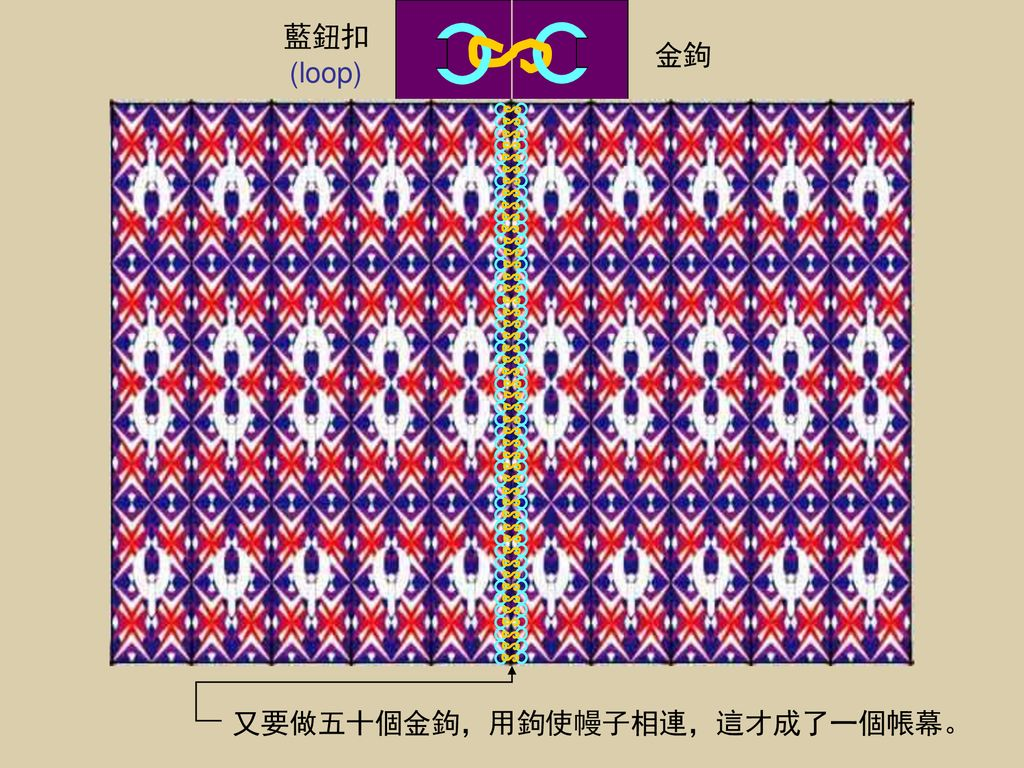
\includegraphics[width=.8\linewidth]{AMoXiFigs/chuaiji/zhangmu1}
%  \caption{A subfigure}
  \label{fig:sub2}
\end{subfigure}
\caption{幕板}
\label{fig:test}
\end{figure}

\begin{figure}[ht]
\centering
\begin{subfigure}{.5\textwidth}
  \centering
  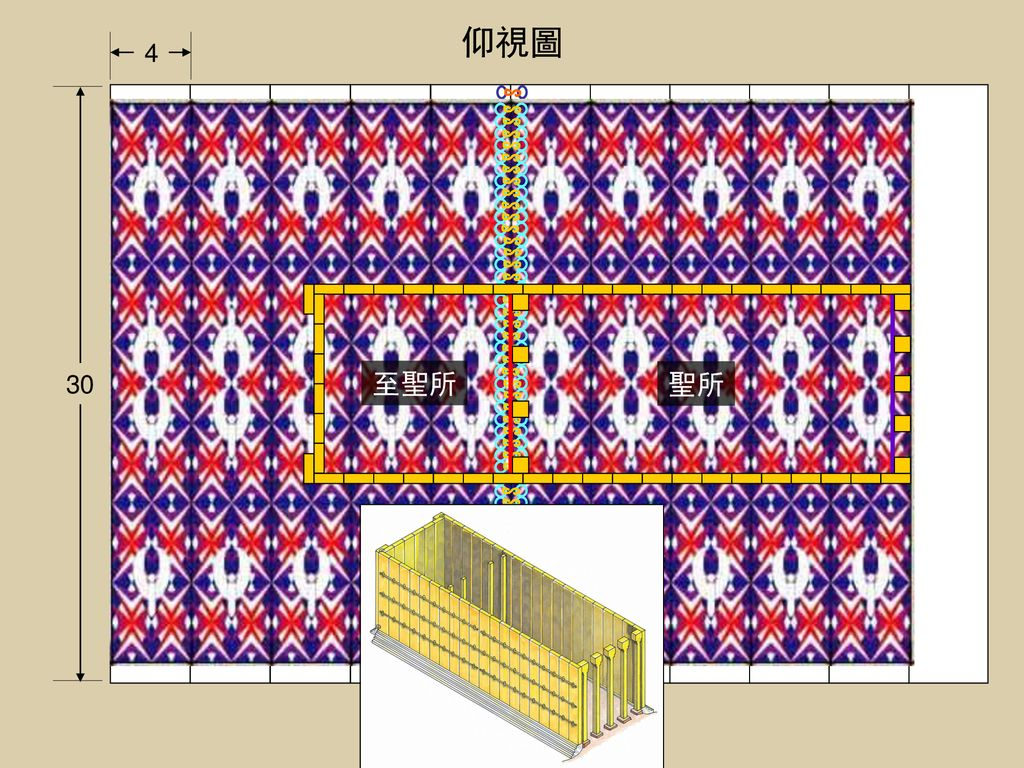
\includegraphics[width=.8\linewidth]{AMoXiFigs/chuaiji/zhangmu4}
 % \caption{A subfigure}
  \label{fig:sub1}
\end{subfigure}%
\begin{subfigure}{.5\textwidth}
  \centering
  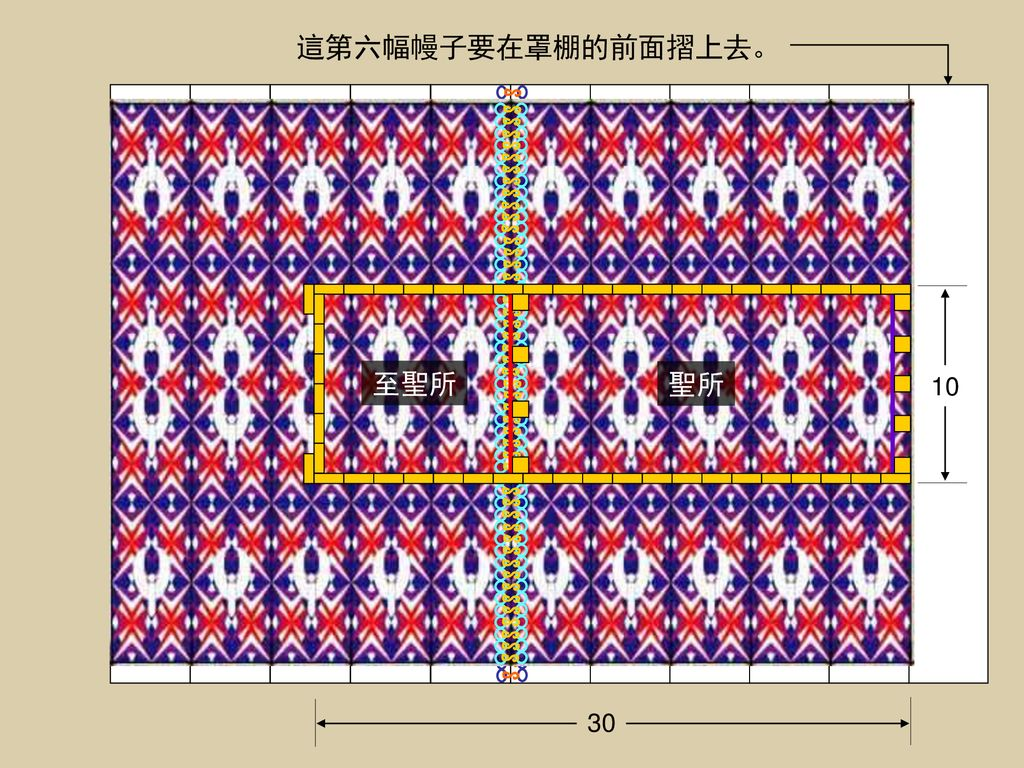
\includegraphics[width=.8\linewidth]{AMoXiFigs/chuaiji/zhangmu6}
%  \caption{A subfigure}
  \label{fig:sub2}
\end{subfigure}
\caption{幕板}
\label{fig:test}
\end{figure}
\begin{figure}[ht]
\centering
\begin{subfigure}{.5\textwidth}
  \centering
  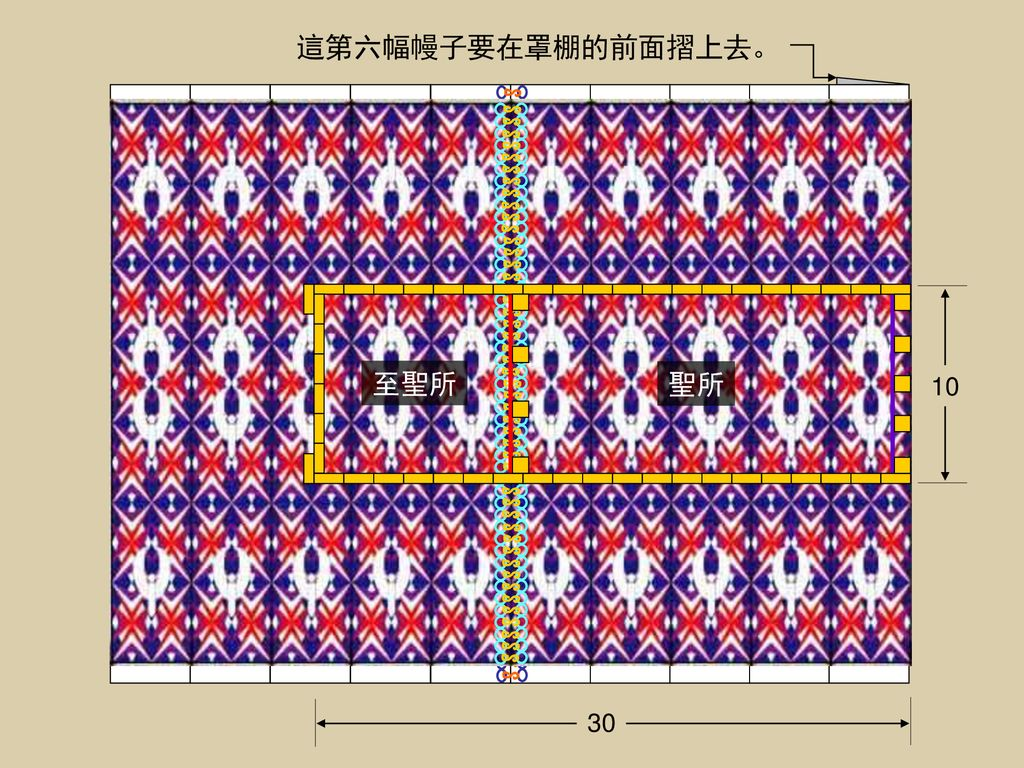
\includegraphics[width=.8\linewidth]{AMoXiFigs/chuaiji/zhangmu7}
 % \caption{A subfigure}
  \label{fig:sub1}
\end{subfigure}%
\begin{subfigure}{.5\textwidth}
  \centering
  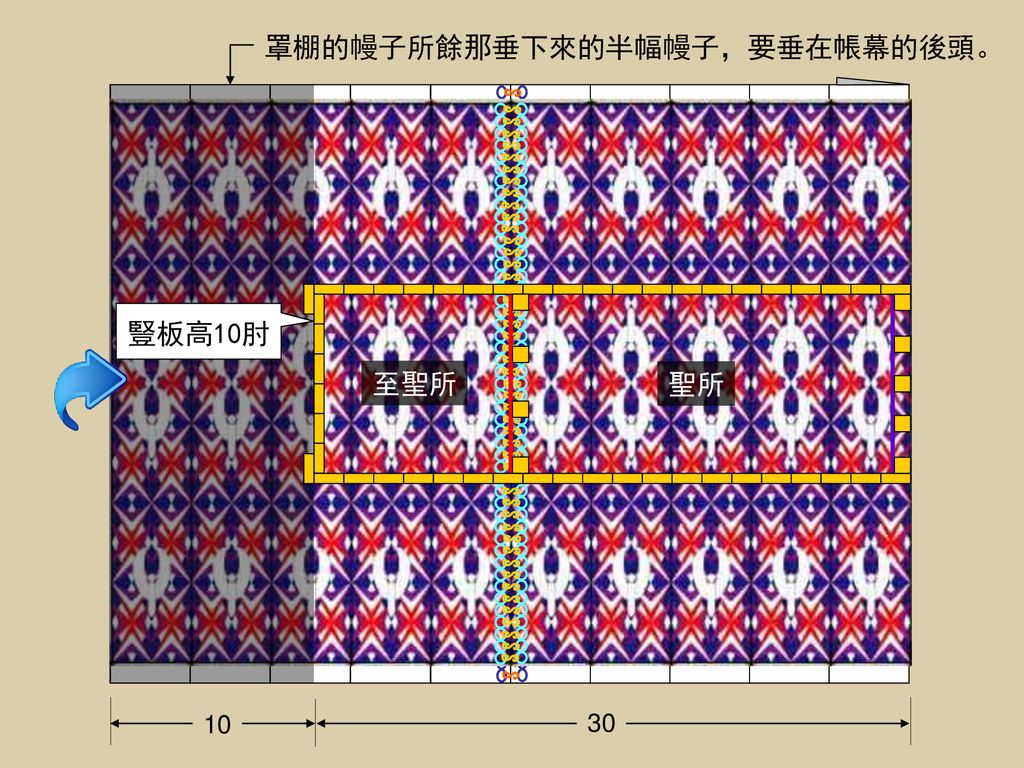
\includegraphics[width=.8\linewidth]{AMoXiFigs/chuaiji/zhangmu8}
%  \caption{A subfigure}
  \label{fig:sub2}
\end{subfigure}
\caption{幕板}
\label{fig:test}
\end{figure}
\begin{figure}[ht]
\centering
\begin{subfigure}{.5\textwidth}
  \centering
  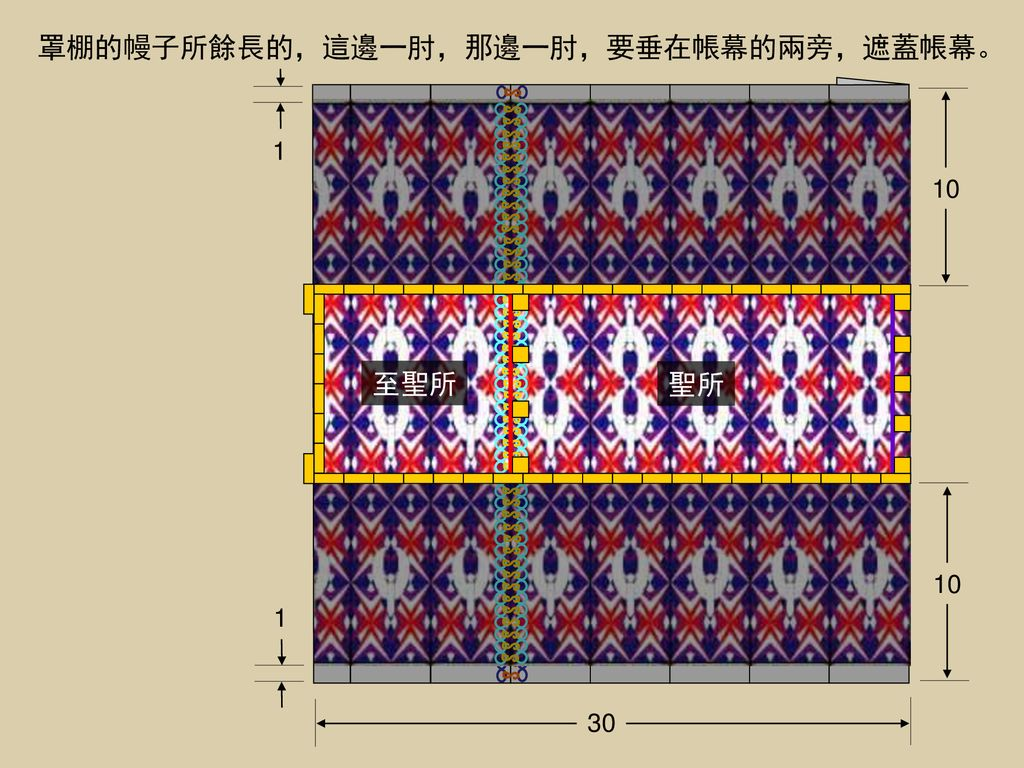
\includegraphics[width=.8\linewidth]{AMoXiFigs/chuaiji/zhangmu9}
 % \caption{A subfigure}
  \label{fig:sub1}
\end{subfigure}%
\begin{subfigure}{.5\textwidth}
  \centering
  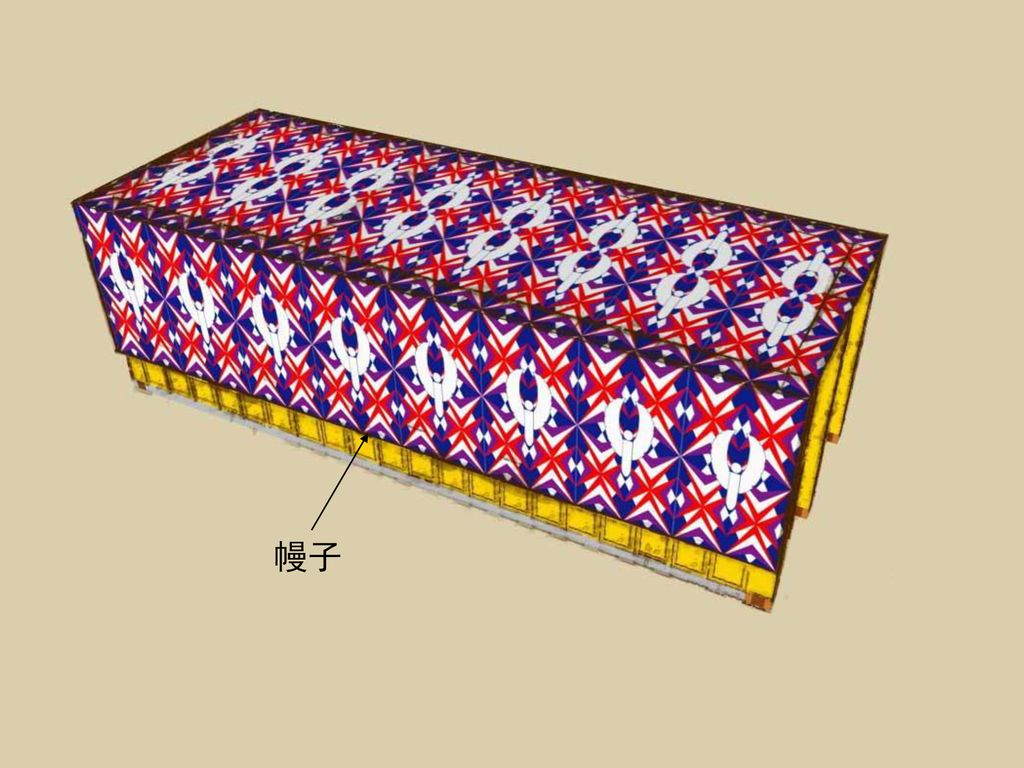
\includegraphics[width=.8\linewidth]{AMoXiFigs/chuaiji/zhangmu11}
%  \caption{A subfigure}
  \label{fig:sub2}
\end{subfigure}
\caption{幕板}
\label{fig:test}
\end{figure}



\subsubsection{造會幕的罩篷 36:14-19}
\begin{figure}[ht]
\centering
\begin{subfigure}{.5\textwidth}
  \centering
  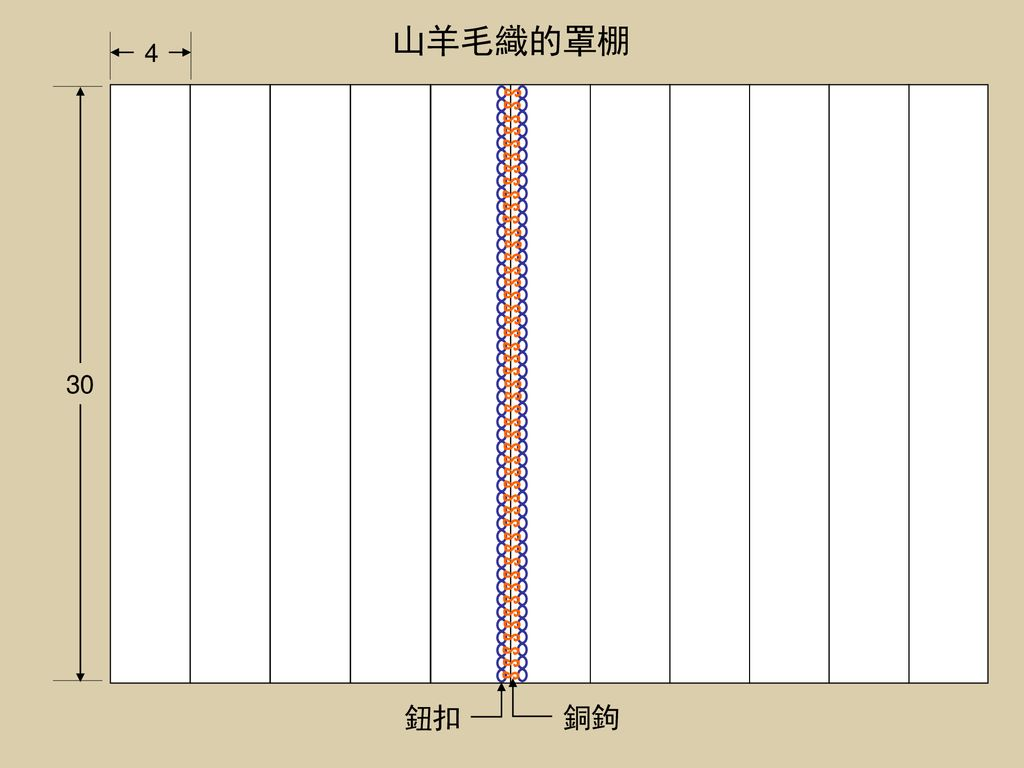
\includegraphics[width=.8\linewidth]{AMoXiFigs/chuaiji/woolcover2}
 % \caption{A subfigure}
  \label{fig:sub1}
\end{subfigure}%
\begin{subfigure}{.5\textwidth}
  \centering
  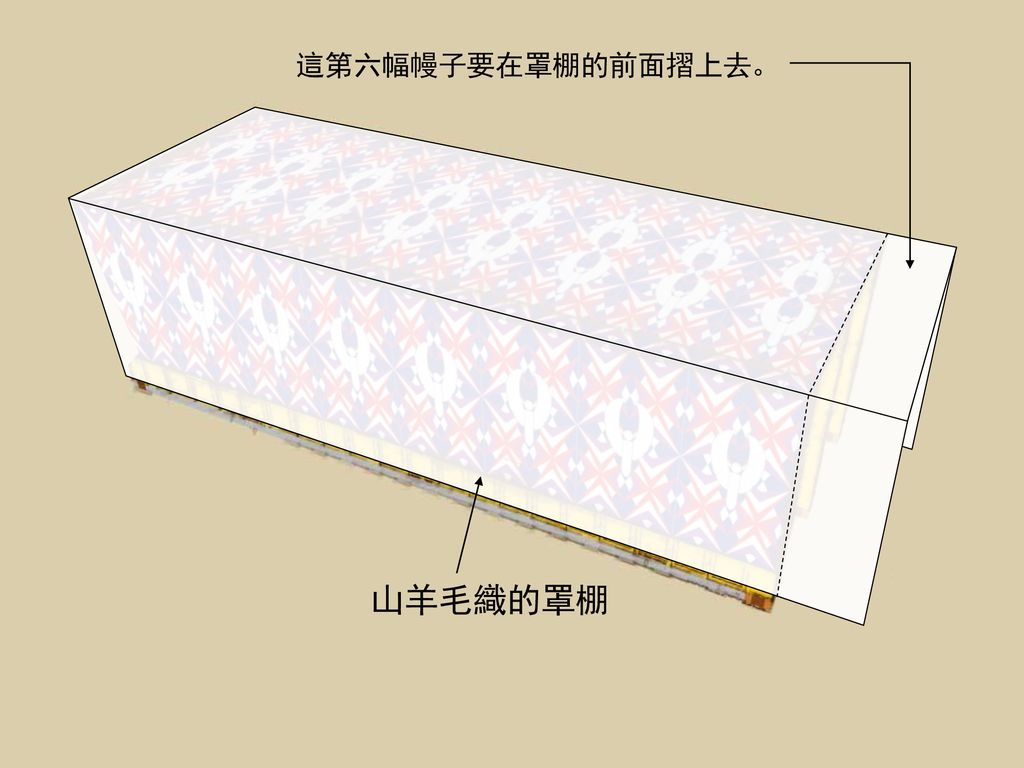
\includegraphics[width=.8\linewidth]{AMoXiFigs/chuaiji/woolcover13}
%  \caption{A subfigure}
  \label{fig:sub2}
\end{subfigure}
\caption{會幕的罩篷}
\label{fig:test}
\end{figure}

\begin{figure}[ht]
\centering
\begin{subfigure}{.5\textwidth}
  \centering
  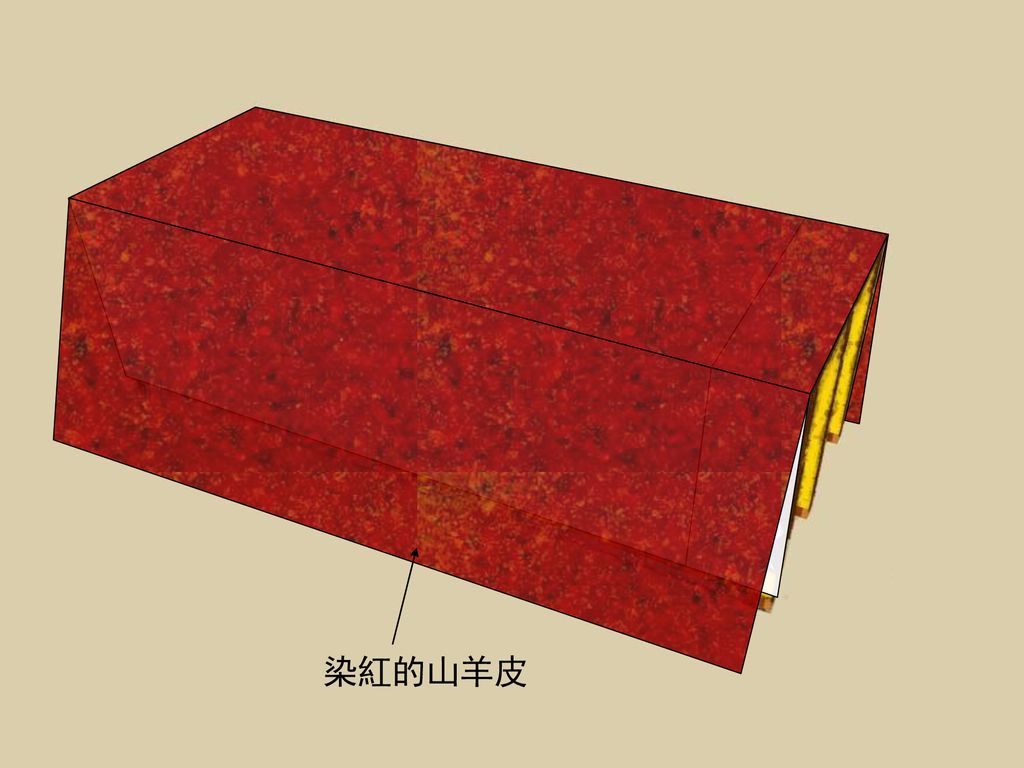
\includegraphics[width=.8\linewidth]{AMoXiFigs/chuaiji/woolcover15}
 % \caption{A subfigure}
  \label{fig:sub1}
\end{subfigure}%
\begin{subfigure}{.5\textwidth}
  \centering
  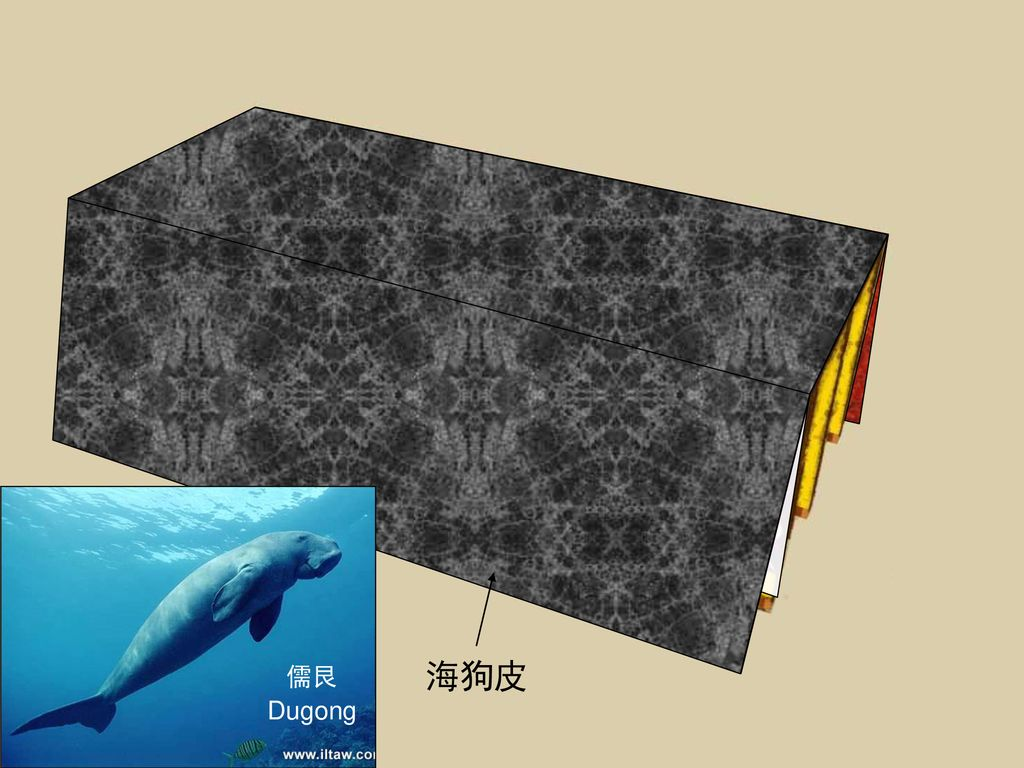
\includegraphics[width=.8\linewidth]{AMoXiFigs/chuaiji/woolcover16}
%  \caption{A subfigure}
  \label{fig:sub2}
\end{subfigure}
\caption{會幕的罩篷}
\label{fig:test}
\end{figure}

\begin{wrapfigure}{r}{0.3\textwidth}
  \centering
  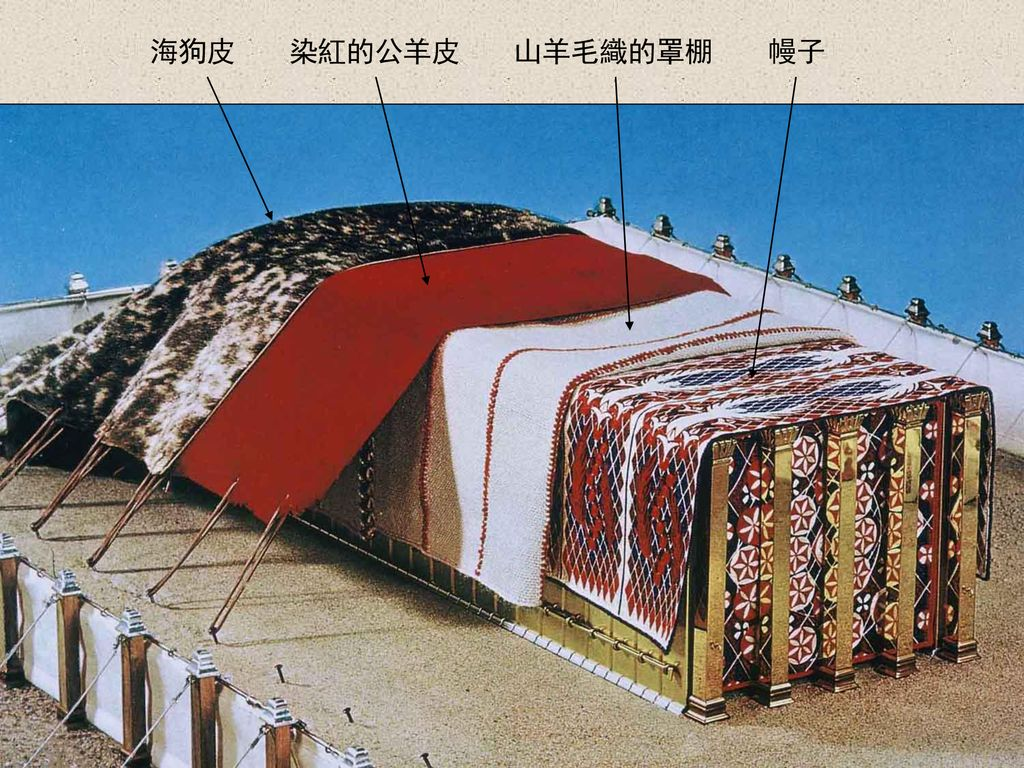
\includegraphics[width=.6\linewidth]{AMoXiFigs/chuaiji/woolcover17}
  \label{fig:sub2}
\caption{會幕的罩篷}
\label{fig:test}
\end{wrapfigure}
他用山羊毛織十一幅幔子，作為帳幕以上的罩篷。每幅幔子長三十肘，寬四肘，十一幅幔子都是一樣的尺寸。 他把五幅幔子連成一幅，又把六幅幔子連成一幅。在這相連的幔子末幅邊上做五十個紐扣，在那相連的幔子末幅邊上也做五十個紐扣。又做五十個銅鉤，使罩篷連成一個。並用染紅的公羊皮做罩篷的蓋，再用海狗皮做一層罩篷上的頂蓋。

\subsubsection{造帳幕的豎板和帶卯的銀座 36:20-34}
\begin{figure}[ht]
\centering
\hspace*{-25mm}
\begin{subfigure}{.33\textwidth}
  \centering
  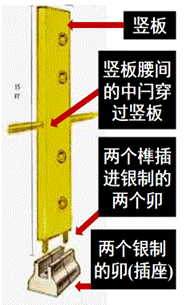
\includegraphics[width=.5\linewidth]{AMoXiFigs/chuaiji/shuban}
 % \caption{A subfigure}
  \label{fig:sub1}
\end{subfigure}%
%\hspace*{ 5mm}
\begin{subfigure}{.33\textwidth}
  \centering
  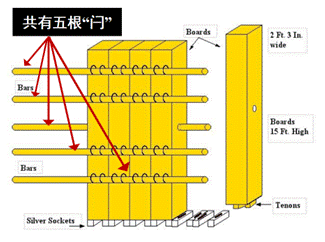
\includegraphics[width=1\linewidth]{AMoXiFigs/chuaiji/shuban1}
%  \caption{A subfigure}
  \label{fig:sub2}
\end{subfigure}
\hspace*{9mm}
\begin{subfigure}{.33\textwidth}
  \centering
  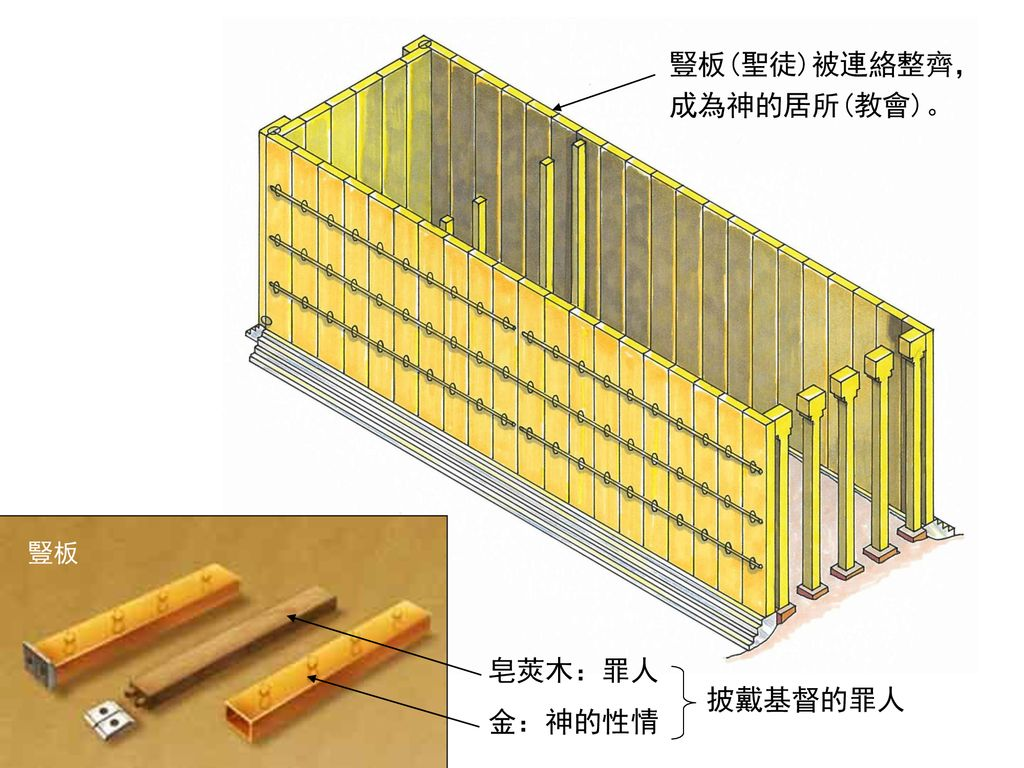
\includegraphics[width=1\linewidth]{AMoXiFigs/chuaiji/shuban2}
%  \caption{A subfigure}
  \label{fig:sub2}
\end{subfigure}
\caption{帳幕的豎板}
\label{fig:test}
\end{figure}


\begin{figure}[ht]
\centering
\begin{subfigure}{.4\textwidth}
  \centering
  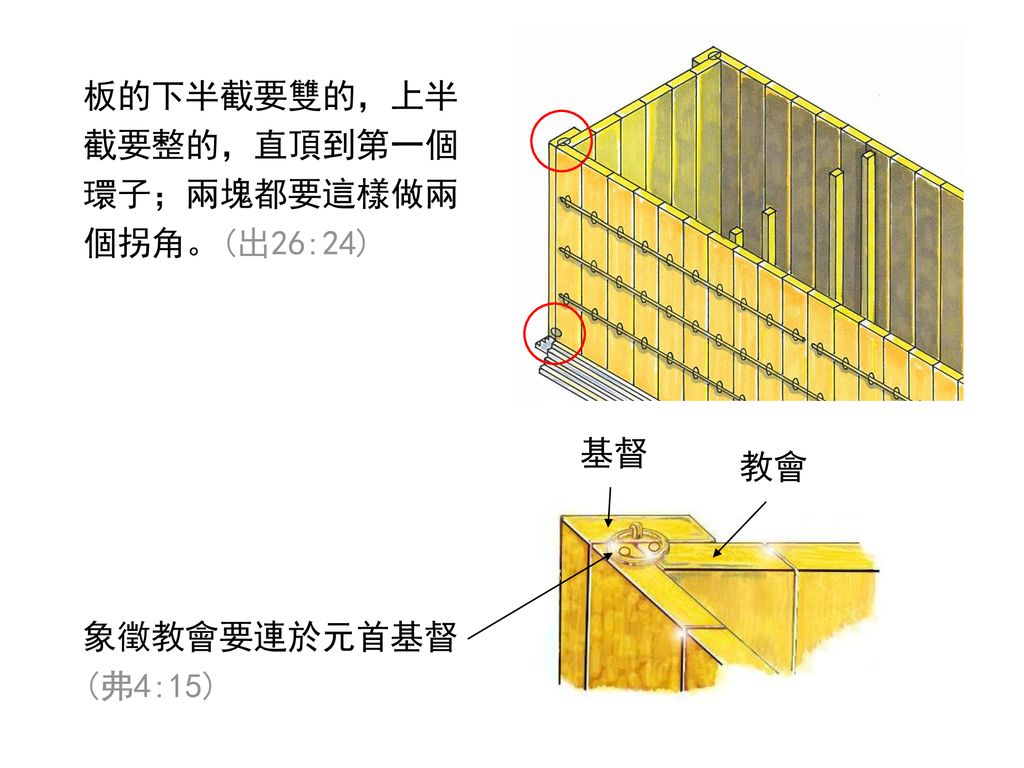
\includegraphics[width=.9\linewidth]{AMoXiFigs/chuaiji/mao}
 % \caption{A subfigure}
  \label{fig:sub1}
\end{subfigure}%
\hspace*{-20mm}
\begin{subfigure}{.4\textwidth}
  \centering
  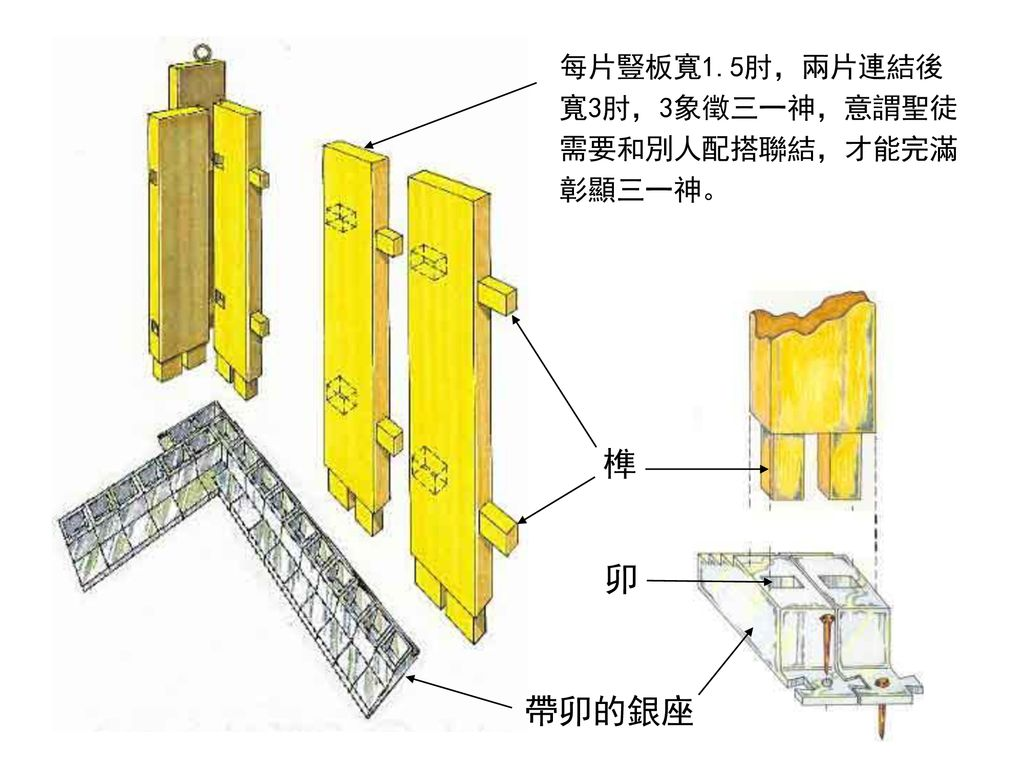
\includegraphics[width=.9\linewidth]{AMoXiFigs/chuaiji/mao3}
%  \caption{A subfigure}
  \label{fig:sub2}
\end{subfigure}
\hspace*{-20mm}
\begin{subfigure}{.4\textwidth}
  \centering
  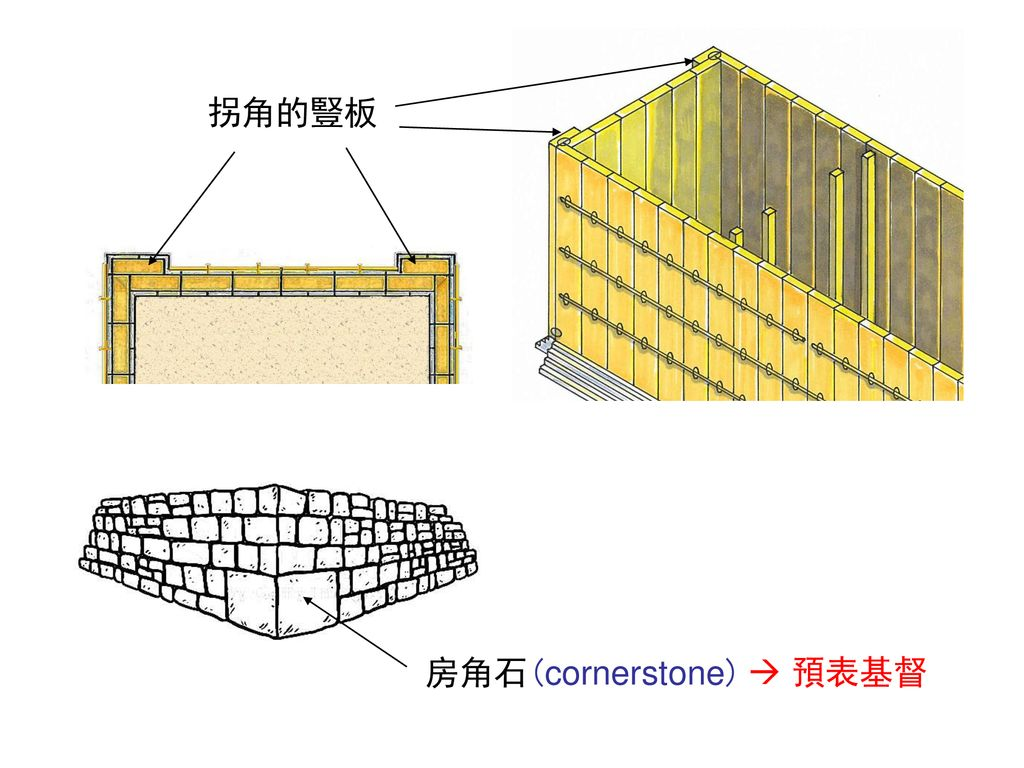
\includegraphics[width=.9\linewidth]{AMoXiFigs/chuaiji/mao5}
%  \caption{A subfigure}
  \label{fig:sub2}
\end{subfigure}
\caption{拐角的豎板}
\label{fig:test}
\end{figure}
他用皂莢木做帳幕的豎板。每塊長十肘，寬一肘半，每塊有兩榫相對。帳幕一切的板都是這樣做。帳幕的南面做板二十塊，在這二十塊板底下又做四十個帶卯的銀座，兩卯接這塊板上的兩榫，兩卯接那塊板上的兩榫。帳幕的第二面，就是北面，也做板二十塊，和帶卯的銀座四十個，這板底下有兩卯，那板底下也有兩卯。帳幕的後面，就是西面，做板六塊。\\
帳幕後面的拐角做板兩塊，板的下半截是雙的，上半截是整的，直到第一個環子，在帳幕的兩個拐角上都是這樣做。有八塊板和十六個帶卯的銀座，每塊板底下有兩卯。他用皂莢木做閂，為帳幕這面的板做五閂， 為帳幕那面的板做五閂，又為帳幕後面的板做五閂，使板腰間的中閂從這一頭通到那一頭。用金子將板包裹，又做板上的金環套閂，閂也用金子包裹。

\subsubsection{造簾 36:35-38}
\begin{wrapfigure}{r}{0.35\textwidth}
\vspace*{-17mm}
%\vspace*{-\baselineskip}
\hspace*{-25mm}
\begin{subfigure}{.5\textwidth}
  \centering
  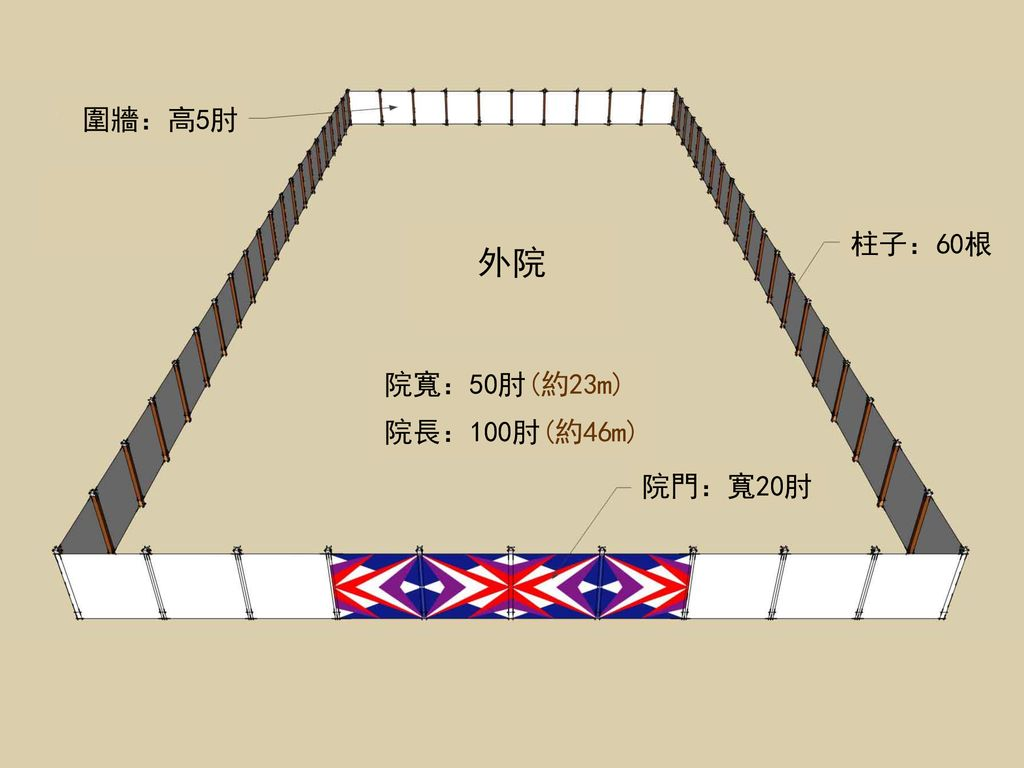
\includegraphics[width=.3\linewidth]{AMoXiFigs/chuaiji/waiyuan}
 % \caption{A subfigure}
  \label{fig:sub1}
\end{subfigure}%
\hspace*{-55mm}
\begin{subfigure}{.5\textwidth}
  \centering
   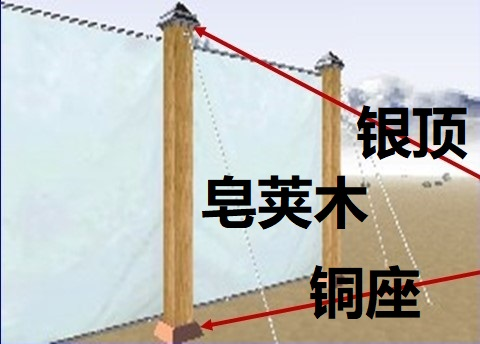
\includegraphics[width=0.32\textwidth]{AMoXiFigs/chuaiji/zhuzi1}
%  \caption{A subfigure}
  \label{fig:sub2}
\end{subfigure}

 % \begin{center}
 %   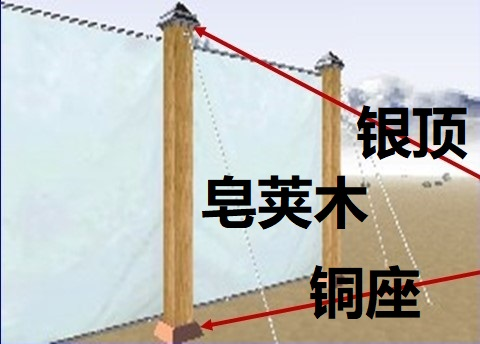
\includegraphics[width=0.16\textwidth]{AMoXiFigs/chuaiji/zhuzi1}
 % \end{center}
%\vspace*{-\baselineskip}
  \caption{簾子}
\end{wrapfigure}
他用藍色、紫色、朱紅色線和撚的細麻織幔子，以巧匠的手工繡上基路伯。為幔子做四根皂莢木柱子，用金包裹，柱子上有金鉤，又為柱子鑄了四個帶卯的銀座。拿藍色、紫色、朱紅色線和撚的細麻，用繡花的手工織帳幕的門簾，又為簾子做五根柱子和柱子上的鉤子，用金子把柱頂和柱子上的杆子包裹。柱子有五個帶卯的座，是銅的。

\subsubsection{造法櫃 37:1-9}
\begin{wrapfigure}{r}{0.35\textwidth}
\vspace*{-17mm}
\hspace*{0mm}
  \centering
  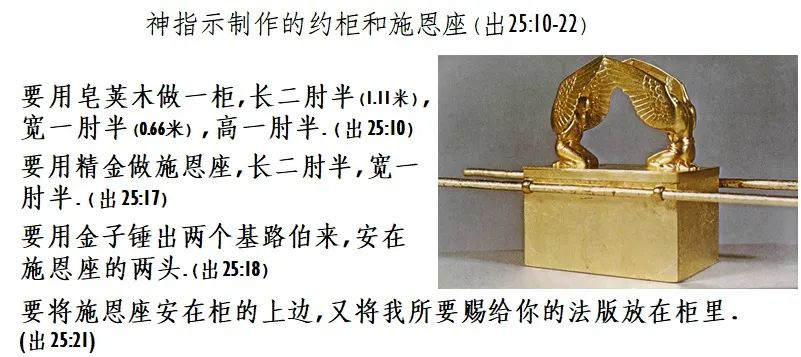
\includegraphics[width=1\linewidth]{AMoXiFigs/chuaiji/yuegui}
  \label{fig:sub1}
\vspace*{-5mm}
  \caption{法櫃 }
\end{wrapfigure}
比撒列用皂莢木做櫃，長二肘半，寬一肘半，高一肘半，裡外包上精金，四圍鑲上金牙邊。又鑄四個金環，安在櫃的四腳上，這邊兩環，那邊兩環。用皂莢木做兩根槓，用金包裹。把槓穿在櫃旁的環內，以便抬櫃。用精金做施恩座，長二肘半，寬一肘半。用金子錘出兩個基路伯來，安在施恩座的兩頭，這頭做一個基路伯，那頭做一個基路伯，二基路伯接連一塊，在施恩座的兩頭。二基路伯高張翅膀，遮掩施恩座，基路伯是臉對臉，朝著施恩座。

\subsubsection{造桌 37:10-16}
他用皂莢木做一張桌子，長二肘，寬一肘，高一肘半，又包上精金，四圍鑲上金牙邊。桌子的四圍各做一掌寬的橫梁，橫梁上鑲著金牙邊。又鑄了四個金環，安在桌子四腳的四角上。安環子的地方是挨近橫梁，可以穿槓抬桌子。他用皂莢木做兩根槓，用金包裹，以便抬桌子。又用精金做桌子上的器皿，就是盤子，調羹，並奠酒的瓶和爵。

\subsubsection{造燈臺 37:17-24}
\begin{wrapfigure}{r}{0.18\textwidth}
\vspace*{-10mm}
%\vspace*{-\baselineskip}
  \begin{center}
    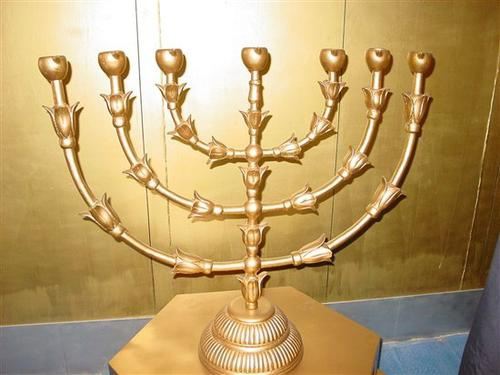
\includegraphics[width=0.18\textwidth]{AMoXiFigs/chuaiji/jindengtai}
  \end{center}
\vspace*{-2mm}
  \caption{燈臺}
\end{wrapfigure}
他用精金做一個燈臺，這燈臺的座和幹與杯、球、花，都是接連一塊錘出來的。燈臺兩旁杈出六個枝子，這旁三個，那旁三個。這旁每枝上有三個杯，形狀像杏花，有球有花；那旁每枝上也有三個杯，形狀像杏花，有球有花。從燈臺杈出來的六個枝子都是如此。 燈臺上有四個杯，形狀像杏花，有球有花。燈臺每兩個枝子以下有球，與枝子接連一塊，燈臺杈出的六個枝子都是如此。球和枝子是接連一塊，都是一塊精金錘出來的。用精金做燈臺的七個燈盞，並燈臺的蠟剪和蠟花盤。他用精金一他連得做燈臺和燈臺的一切器具。

\subsubsection{造香壇 37:25-29}
他用皂莢木做香壇，是四方的，長一肘，寬一肘，高二肘，壇的四角與壇接連一塊。又用精金把壇的上面與壇的四面並壇的四角包裹，又在壇的四圍鑲上金牙邊。做兩個金環，安在牙子邊以下，在壇的兩旁兩根橫撐上，作為穿槓的用處，以便抬壇。用皂莢木做槓，用金包裹。又按做香之法做聖膏油和馨香料的淨香。

\subsubsection{造祭壇 38:1-7}
\begin{wrapfigure}{r}{0.7\textwidth}
\vspace*{-5mm}
%\begin{figure}[ht]
\centering
\begin{subfigure}{.5\textwidth}
  \centering
  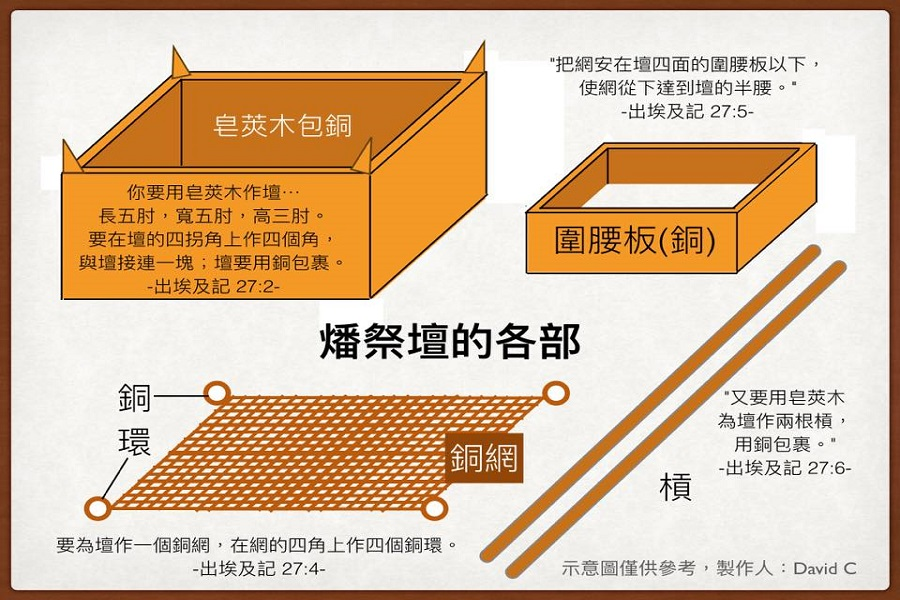
\includegraphics[width=.7\linewidth]{AMoXiFigs/chuaiji/jitan}
 % \caption{A subfigure}
  \label{fig:sub1}
\end{subfigure}%
\hspace*{-30mm}
\begin{subfigure}{.5\textwidth}
  \centering
  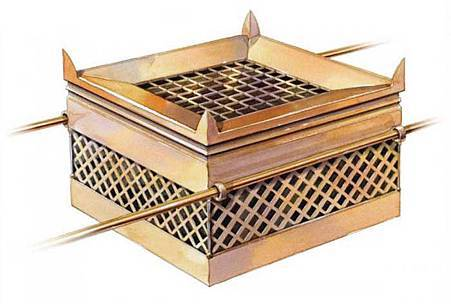
\includegraphics[width=.6\linewidth]{AMoXiFigs/chuaiji/jitan3}
%  \caption{A subfigure}
  \label{fig:sub2}
\end{subfigure}
\caption{祭壇}
\label{fig:test}
\end{wrapfigure}
他用皂莢木做燔祭壇，是四方的，長五肘，寬五肘，高三肘。在壇的四拐角上做四個角，與壇接連一塊，用銅把壇包裹。他做壇上的盆、鏟子、盤子、肉叉子、火鼎，這一切器具都是用銅做的。又為壇做一個銅網，安在壇四面的圍腰板以下，從下達到壇的半腰。為銅網的四角鑄四個環子，作為穿槓的用處。 用皂莢木做槓，用銅包裹，把槓穿在壇兩旁的環子內，用以抬壇；並用板做壇，壇是空的。

\subsubsection{造浴盆 38:8}
他用銅做洗濯盆和盆座，是用會幕門前伺候的婦人之鏡子做的。

\subsubsection{立幕院 38:9-20}

他做帳幕的院子。院子的南面用撚的細麻做帷子，寬一百肘。帷子的柱子二十根，帶卯的銅座二十個，柱子上的鉤子和杆子都是用銀子做的。北面也有帷子，寬一百肘。帷子的柱子二十根，帶卯的銅座二十個，柱子上的鉤子和杆子都是用銀子做的。院子的西面有帷子，寬五十肘。帷子的柱子十根，帶卯的座十個，柱子的鉤子和杆子都是用銀子做的。院子的東面，寬五十肘。門這邊的帷子十五肘，那邊也是一樣。帷子的柱子三根，帶卯的座三個。在門的左右各有帷子十五肘，帷子的柱子三根，帶卯的座三個。院子四面的帷子都是用撚的細麻做的。柱子帶卯的座是銅的，柱子上的鉤子和杆子是銀的，柱頂是用銀子包的。院子一切的柱子都是用銀杆連絡的。院子的門簾是以繡花的手工，用藍色、紫色、朱紅色線和撚的細麻織的，寬二十肘，高五肘，與院子的帷子相配。帷子的柱子四根，帶卯的銅座四個，柱子上的鉤子和杆子是銀的，柱頂是用銀子包的。帳幕一切的橛子和院子四圍的橛子都是銅的。

\subsubsection{核記民獻金銀銅之數 38:21-31}

這是法櫃的帳幕中利未人所用物件的總數，是照摩西的吩咐，經祭司亞倫的兒子以他瑪的手數點的。凡耶和華所吩咐摩西的，都是猶大支派戶珥的孫子、烏利的兒子比撒列做的。與他同工的有但支派中亞希撒抹的兒子亞何利亞伯，他是雕刻匠，又是巧匠，又能用藍色、紫色、朱紅色線和細麻繡花。

\begin{wraptable}{r}{14.5cm}
%\begin{table}[H]
\vspace*{-\baselineskip}
\center
\begin{tabular}{ c c l }
\toprule
材料 &重量 &用途\\\hline
所獻的金子&29他連得730舍客勒 &  \\\hline
被數人所出的銀子&100他連得 &100帶卯的座,1他連得/帶卯的座\\
0.5舍客勒/被數人 &1775舍客勒&做柱子上的鉤子，包裹柱頂並柱子上的杆子\\\hline
銅 &70他連得2400舍客勒&會幕門帶卯的座,銅壇並壇上的銅網並一切器具\\
   &                               &院子四圍,院門帶卯的座,帳幕和院子四圍的橛子\\\hline
\end{tabular}
\caption{技工比撒列,亞何利亞伯}
%\end{table} 
\end{wraptable}
為聖所一切工作使用所獻的\textcolor{blue}{金子}，按聖所的平，有二十九他連得並七百三十舍客勒。會中被數的人所出的\textcolor{blue}{銀子}，按聖所的平，有一百他連得並一千七百七十五舍客勒。凡過去歸那些被數之人的，從二十歲以外，有六十萬零三千五百五十人，按聖所的平，每人出銀半舍客勒，就是一比加。用那一百他連得銀子鑄造聖所帶卯的座和幔子柱子帶卯的座，一百他連得共一百帶卯的座，每帶卯的座用一他連得。用那一千七百七十五舍客勒銀子做柱子上的鉤子，包裹柱頂並柱子上的杆子。所獻的\textcolor{blue}{銅}有七十他連得並二千四百舍客勒。 用這銅做會幕門帶卯的座和銅壇，並壇上的銅網和壇的一切器具，並院子四圍帶卯的座和院門帶卯的座，與帳幕一切的橛子和院子四圍所有的橛子。

\subsubsection{造會幕所用的金屬 39:1-7}
比撒列用藍色、紫色、朱紅色線做精緻的衣服，在聖所用以供職，又為亞倫做聖衣，是照耶和華所吩咐摩西的。他用金線和藍色、紫色、朱紅色線並撚的細麻做以弗得。把金子錘成薄片，剪出線來，與藍色、紫色、朱紅色線，用巧匠的手工一同繡上。又為以弗得做兩條相連的肩帶，接連在以弗得的兩頭。其上巧工織的帶子和以弗得一樣的做法，用以束上，與以弗得接連一塊，是用金線和藍色、紫色、朱紅色線並撚的細麻做的，是照耶和華所吩咐摩西的。
又琢出兩塊紅瑪瑙，鑲在金槽上，彷彿刻圖書，按著以色列兒子的名字雕刻，將這兩塊寶石安在以弗得的兩條肩帶上，為以色列人做紀念石，是照耶和華所吩咐摩西的。

\subsubsection{做胸牌 39:8-21}
他用巧匠的手工做胸牌，和以弗得一樣的做法，用金線與藍色、紫色、朱紅色線並撚的細麻做的。胸牌是四方的，疊為兩層，這兩層長一虎口，寬一虎口，上面鑲著寶石四行：第一行是紅寶石、紅璧璽、紅玉， 第二行是綠寶石、藍寶石、金鋼石，第三行是紫瑪瑙、白瑪瑙、紫晶，第四行是水蒼玉、紅瑪瑙、碧玉。這都鑲在金槽中。 14 這些寶石都是按著以色列十二個兒子的名字，彷彿刻圖書，刻十二個支派的名字。在胸牌上，用精金擰成如繩子的鏈子。又做兩個金槽和兩個金環，安在胸牌的兩頭。 把那兩條擰成的金鏈子穿過胸牌兩頭的環子，又把鏈子的那兩頭接在兩槽上，安在以弗得前面肩帶上。做兩個金環，安在胸牌的兩頭，在以弗得裡面的邊上。 又做兩個金環，安在以弗得前面兩條肩帶的下邊，挨近相接之處，在以弗得巧工織的帶子以上。用一條藍細帶子把胸牌的環子和以弗得的環子繫住，使胸牌貼在以弗得巧工織的帶子上，不可與以弗得離縫，是照耶和華所吩咐摩西的。

\subsubsection{做外袍 39:22-26}
他用織工做以弗得的外袍，顏色全是藍的。袍上留一領口，口的周圍織出領邊來，彷彿鎧甲的領口，免得破裂。在袍子底邊上，用藍色、紫色、朱紅色線並撚的細麻做石榴。又用精金做鈴鐺，把鈴鐺釘在袍子周圍底邊上的石榴中間：一個鈴鐺，一個石榴，一個鈴鐺，一個石榴，在袍子周圍底邊上，用以供職，是照耶和華所吩咐摩西的。

\subsubsection{做內袍 39:27-29}
他用織成的細麻布為亞倫和他的兒子做內袍，並用細麻布做冠冕和華美的裹頭巾，用撚的細麻布做褲子，又用藍色、紫色、朱紅色線並撚的細麻，以繡花的手工做腰帶，是照耶和華所吩咐摩西的。

\subsubsection{造冕牌 39:30-31}
他用精金做聖冠上的牌，在上面按刻圖書之法，刻著：歸耶和華為聖。又用一條藍細帶子將牌繫在冠冕上，是照耶和華所吩咐摩西的。

%\subsection{造會幕竣工 36:8-39:31}
\subsubsection{幕工告竣 39:32-43}
帳幕，就是會幕，一切的工就這樣做完了。凡耶和華所吩咐摩西的，以色列人都照樣做了。他們送到摩西那裡，帳幕和帳幕的一切器具，就是鉤子、板、閂、柱子、帶卯的座，染紅公羊皮的蓋、海狗皮的頂蓋和遮掩櫃的幔子，法櫃和櫃的槓並施恩座，桌子和桌子的一切器具並陳設餅， 精金的燈臺和擺列的燈盞與燈臺的一切器具並點燈的油， 金壇，膏油，馨香的香料，會幕的門簾，銅壇和壇上的銅網，壇的槓並壇的一切器具，洗濯盆和盆座，院子的帷子和柱子，並帶卯的座，院子的門簾、繩子、橛子，並帳幕和會幕中一切使用的器具，精工做的禮服和祭司亞倫並他兒子在聖所用以供祭司職分的聖衣。這一切工作都是以色列人照耶和華所吩咐摩西做的。耶和華怎樣吩咐的，他們就怎樣做了。摩西看見一切的工都做成了，就給他們祝福


\subsubsection{命摩西建會幕 40:1-16}
耶和華曉諭摩西說： 「正月初一日，你要立起帳幕，把法櫃安放在裡面，用幔子將櫃遮掩。把桌子搬進去，擺設上面的物。把燈臺搬進去，點其上的燈。把燒香的金壇安在法櫃前，掛上帳幕的門簾。把燔祭壇安在帳幕門前。把洗濯盆安在會幕和壇的中間，在盆裡盛水。又在四圍立院帷，把院子的門簾掛上。 用膏油把帳幕和其中所有的都抹上，使帳幕和一切器具成聖，就都成聖。又要抹燔祭壇和一切器具，使壇成聖，就都成為至聖。要抹洗濯盆和盆座，使盆成聖。要使亞倫和他兒子到會幕門口來，用水洗身。要給亞倫穿上聖衣，又膏他，使他成聖，可以給我供祭司的職分。又要使他兒子來，給他們穿上內袍。怎樣膏他們的父親，也要照樣膏他們，使他們給我供祭司的職分。他們世世代代凡受膏的，就永遠當祭司的職任。」摩西這樣行，都是照耶和華所吩咐他的。


\subsubsection{會幕完工 40:17-33 }
第二年正月初一日，帳幕就立起來。摩西立起帳幕，安上帶卯的座，立上板，穿上閂，立起柱子，在帳幕以上搭罩篷，把罩篷的頂蓋蓋在其上，是照耶和華所吩咐他的。又把法版放在櫃裡，把槓穿在櫃的兩旁，把施恩座安在櫃上。把櫃抬進帳幕，掛上遮掩櫃的幔子，把法櫃遮掩了，是照耶和華所吩咐他的。又把桌子安在會幕內，在帳幕北邊，在幔子外，在桌子上將餅陳設在耶和華面前，是照耶和華所吩咐他的。又把燈臺安在會幕內，在帳幕南邊，與桌子相對，在耶和華面前點燈，是照耶和華所吩咐他的。把金壇安在會幕內的幔子前，在壇上燒了馨香料做的香，是照耶和華所吩咐他的。又掛上帳幕的門簾。在會幕的帳幕門前，安設燔祭壇，把燔祭和素祭獻在其上，是照耶和華所吩咐他的。把洗濯盆安在會幕和壇的中間，盆中盛水，以便洗濯。摩西和亞倫並亞倫的兒子在這盆裡洗手洗腳。他們進會幕或就近壇的時候，便都洗濯，是照耶和華所吩咐他的。在帳幕和壇的四圍立了院帷，把院子的門簾掛上。這樣，摩西就完了工。

\subsubsection{神的榮光在會幕顯現 40:34-38 （民9:15-23 ）}
當時，雲彩遮蓋會幕，耶和華的榮光就充滿了帳幕。摩西不能進會幕，因為雲彩停在其上，並且耶和華的榮光充滿了帳幕。每逢雲彩從帳幕收上去，以色列人就起程前往；雲彩若不收上去，他們就不起程，直等到雲彩收上去。日間，耶和華的雲彩是在帳幕以上；夜間，雲中有火，在以色列全家的眼前。在他們所行的路上，都是這樣。



















